\documentclass[10pt]{memoir}
\setstocksize{220mm}{155mm} 	        
\settrimmedsize{220mm}{155mm}{*}	
\settypeblocksize{170mm}{116mm}{*}	
\setlrmargins{18mm}{*}{*}
\setulmargins{*}{*}{1.2}
%\setlength{\headheight}{5pt}%
\checkandfixthelayout[lines]
\linespread{1.16}
\flushbottom

%%% Hyphenation settings
\usepackage[htt]{hyphenat}
\hyphenation{he-lio-trope opos-sum}
\tracingparagraphs=1
%Hyphenation in Devanāgarī of the edition still missing? Probably this needs to be modified in babel-iast package? 

%%% babel
\usepackage[english]{babel}
\usepackage{babel-iast/babel-iast}

\babelfont[iast]{rm}[Renderer=Harfbuzz, Scale=1.3]{AdishilaSan}%AdishilaSan}
\babelfont[english]{rm}{Adobe Text Pro}

%%% more functionality
\PassOptionsToPackage{hyphens}{url}
\usepackage{hyperref}
\usepackage{pdflscape}
\usepackage{cleveref}
\usepackage{url}
\usepackage{cleveref}
\usepackage{microtype}
\usepackage{lineno}

%\usepackage{bigfoot}
%%% more functions
\usepackage[dvipsnames]{xcolor}
%\usepackage[para,perpage]{footmisc}

%%%für den Counter von Kapiteln und Sätzen! 
\newcommand{\uproman}[1]{\uppercase\expandafter{\romannumeral#1}}
\newcommand{\lowroman}[1]{\romannumeral#1\relax}

\makeindex
\newfontfamily\sanskritfont[Script=Devanagari,Mapping=RomDev,Scale=1.1]{Sanskrit2003}
\usepackage{pifont,fourier-orns,lettrine,psvectorian,paralist,enumitem,pdfpages,wrapfig,tabulary,lettrine,longtable}
\setlist[enumerate]{itemsep=0mm}
\usepackage[autostyle]{csquotes}
\usepackage[defaultlines=2,all]{nowidow}
\usepackage{ellipsis,adforn,booktabs,longtable,url,tikz}
\lineskiplimit=-3pt          

\makechapterstyle{IeT}{%
  \chapterstyle{default}
  \renewcommand*{\printchapternonum}{\centering}
  \renewcommand*{\clearforchapter}{\cleartorecto} 
  \aliaspagestyle{chapter}{empty}}
\chapterstyle{IeT}
\setsecnumdepth{none}  \openright  \nouppercaseheads
\settocdepth{subsubsection}

%%%% test better pagebreaks
%\def\fussy{%
%  \emergencystretch\z@
%  \tolerance 200%
%  \hfuzz .1\p@
%  \vfuzz\hfuzz}

%\interfootnotelinepenalty=10000\relax

%\usepackage[maxfloats=256]{morefloats}

%\maxdeadcycles=500

%raggedbottomsectiontrue
%%\checkandfixthelayout


%%%%%%%  biblatex
%\newcommand{\noun}[1]{\textsc{#1}}    %  philosophy-verbose
\usepackage[backend=biber, sorting=nyt, style=verbose]{biblatex} %%%%ORIGINAL TiE
\renewcommand*{\mkbibnamefamily}[1]{\textsc{#1}}


\DeclareFieldFormat{url}{%
  \mkbibacro{URL}\addcolon\space
  \href{#1}{\nolinkurl{\thefield{urlraw}}}}

\DeclareFieldFormat{citeurl}{%
  \href{#1}{\nolinkurl{\thefield{urlraw}}}} 


\DeclareFieldFormat{postnote}{#1}
\renewcommand{\postnotedelim}{, }
\addbibresource{bindu.bib}

%%% ekdosis
\usepackage[teiexport=tidy,parnotes=true]{ekdosis}% =tidy cleans up HTML and XML documents by fixing markup errors and upgrading legacy code to modern standards. parnotes=footnotes below or above critical apparatus

\SetLineation{lineation=page, modulo} %lineation=page sets thenumbering to start afresh at the top of each page. =modulo makes every fifth line numbered. {lineation=page} makes every line numbered! 

\renewcommand{\linenumberfont}{\selectlanguage{english}\footnotesize} %sets language of lines to English

\SetTEIxmlExport{autopar=false} %autopar=falseinstructs ekdosis to ignore blank lines in the.tex sourcefile as markers for paragraph boundaries. As a result, each paragraph of the edition must be found within an environment associated with the xml <p> element

\SetHooks{
  lemmastyle=\bfseries,
  %refnumstyle=\selectlanguage{english}\bfseries,
  refnumstyle=\selectlanguage{english}\color{blue}\bfseries,
  appheight=0.8\textheight,
}

\newif\ifinapparatus
\DeclareApparatus{source}[
%bhook=\inapparatustrue,
lang=english,
notelang=english,
% bhook=\selectlanguage{english},
bhook=\selectlanguage{english}\textbf{Sources:},%
%maxentries=4, 
%ehook=.]
%sep={] },
%nosep,
]

\newif\ifinapparatus
\DeclareApparatus{testium}[
%bhook=\inapparatustrue,
lang=english,
notelang=english,
% bhook=\selectlanguage{english},
bhook=\selectlanguage{english}\textbf{Testimonia:},
%maxentries=4, 
%ehook=.]
%nosep, 
]

% Declare \ifinapparatus and set \inapparatustrue at the beginning of
% the apparatus criticus block. Also set the language.  
\newif\ifinapparatus
  \DeclareApparatus{default}[
  %bhook=\inapparatustrue, 
  lang=english,
  %maxentries=33,
  %bhook=\selectlanguage{english},
  sep = {] },
  delim=\hskip 0.75em,
  rule=\rule{0.7in}{0.4pt},
]

\newif\ifinapparatus
\DeclareApparatus{philcomm}[
%bhook=\inapparatustrue,
lang=english,
notelang=english,
bhook=\selectlanguage{english}\textbf{Philological Commentary:},
%bhook=\selectlanguage{english},
sep={: },
]

\ekdsetup{
showpagebreaks,
spbmk = \textcolor{blue}{spb},
hpbmk = \textcolor{red}{hpb}
}

%\usepackage{fnpos}
%\makeFNmid
%\makeFNbottom
\usepackage[bottom]{footmisc}
%%%%%%%%%%%%%%%%%%%%%%%%%%%
\makeatletter
\def\blfootnote{\gdef\@thefnmark{}\@footnotetext}
\makeatother
%%%%%%%%%%%%%%%%%%%%%%%%%


% Macros and Definitions for the Print of Sigla
\def\acpc#1#2#3{{#1}\rlap{\textrm{\textsuperscript{#3}}}\textsubscript{\textrm{#2}}\space}
\def\sigl#1#2{{{#1}}\textsubscript{\textrm{#2}}}
\def\None{{\sigl{N}{1}}} \def\Noneac{\acpc{N}{1}{ac}\,} \def\Nonepc{\acpc{N}{1}{pc}\,}
\def\Ntwo{{\sigl{N}{2}}} \def\Noneac{\acpc{N}{2}{ac}\,} \def\Nonepc{\acpc{N}{2}{pc}\,}
\def\Done{{\sigl{D}{1}}} \def\Doneac{\acpc{D}{1}{ac}\,} \def\Donepc{\acpc{D}{1}{pc}\,}
\def\Dtwo{{\sigl{D}{2}}} \def\Dtwoac{\acpc{D}{2}{ac}\,} \def\Dtwopc{\acpc{D}{2}{pc}\,}
\def\Uone{{\sigl{U}{1}}} \def\Uoneac{\acpc{U}{1}{ac}\,} \def\Uonepc{\acpc{U}{1}{pc}\,}                 
\def\Utwo{{\sigl{U}{2}}} \def\Utwoac{\acpc{U}{2}{ac}\,} \def\Utwopc{\acpc{U}{2}{pc}\,}

%%%%%%%%%%%%%% Tattvabinduyoga - List of Witnesses   %%%%%%%%%%%%%%%%%%%
\DeclareWitness{ceteri}{\selectlanguage{english}cett.}{ceteri}[]   
\DeclareWitness{E}{\selectlanguage{english}E}{Printed Edition}[]    
\DeclareWitness{P}{\selectlanguage{english}P}{Pune BORI 664}[]  
\DeclareWitness{B}{\selectlanguage{english}B}{Bodleian 485}[]       
\DeclareWitness{N1}{\selectlanguage{english}N\textsubscript{1}}{NGMPP 38/31}[]
\DeclareWitness{N2}{\selectlanguage{english}N\textsubscript{2}}{NGMPP B 38/35}[]
\DeclareWitness{L}{\selectlanguage{english}L}{LALCHAND 5876}[]  
\DeclareWitness{D}{\selectlanguage{english}D}{IGNCA 30019}[] 
%\DeclareWitness{D2}{\selectlanguage{english}D\textsubscript{2}}{IGNCA 30020}[]  
\DeclareWitness{U1}{\selectlanguage{english}U\textsubscript{1}}{SORI 1574}[] 
\DeclareWitness{U2}{\selectlanguage{english}U\textsubscript{2}}{SORI 6082}[]
%%%%%%%%%%%%%% Tattvabinduyoga - Groups of Witnesses   %%%%%%%%%%%%%%%%%%%
\DeclareWitness{X}{\selectlanguage{english}\alpha}{Alpha Group: D,N1,N2,U1}[]
\DeclareWitness{Y}{\selectlanguage{english}\beta}{Beta Group: B,E,L,P,U2}[]
%%%%%%%%%%%%% Testimonia
\DeclareWitness{Ysv}{\selectlanguage{english}Ysv}{Yogasvarodaya}[] %%%add infos!  

%%%%%%%%%%%%%%%%%%%%%%%%%%%%%%%%%%%%%%%%%%%
% Macro for Editing Abbrevs.
\def\om{\textrm{\footnotesize \textit{om.}\ }} %prints om. for omitted in apparatus
\def\korr{\textrm{\footnotesize \textit{em.}\ }} %prints em. for emended in apparatus
\def\conj{\textrm{\footnotesize \textit{conj.}\ }} %prints conj. for conjectured in apparatus

% \supplied{text} EDITORIAL ADDITION -> Within \lem oder \rdg
% \surplus{text} EDITORIAL DELETION -> Within \lem oder \rdg
% \sic{text} CRUX
% \gap{text} LACUNAE -> [reason=??, unit=??, quantity=??, extent=??]


%%%%%%%%%%%%%%%%%%%%%%%%%%%%%%%%%%%%%%%%%%% All macros of this list can be used in 
% Macro for Editing Abbrevs.
\def\eyeskip{\textrm{{ab.\,oc. }}}
\def\aberratio{\textrm{{ab.\,oc. }}}
\def\ad{\textrm{{ad}}}
\def\add{\textrm{{add.\ }}}
\def\ann{\textrm{{ann.\ }}}
\def\ante{\textrm{{ante }}} 
\def\post{\textrm{{post }}}
%\def\ceteri{cett.\,}                   
\def\codd{\textrm{{codd.\ }}}

\def\coni{\textrm{{coni.\ }}}
\def\contin{\textrm{{contin.\ }}}
\def\corr{\textrm{{corr.\ }}}
\def\del{\textrm{{del.\ }}}
\def\dub{\textrm{{ dub.\ }}}

\def\expl{\textrm{{explic.\ }}} 
\def\explica t{\textrm{{explic.\ }}}
\def\fol{\textrm{{fol.\ }}}
\def\foll{\textrm{{foll.\ }}}
\def\gloss{\textrm{{glossa ad }}}
\def\ins{\textrm{{ins.\ }}}      
\def\inseruit{\textrm{{ins.\ }}} 
\def\im{{\kern-.7pt\lower-1ex\hbox{\textrm{\tiny{\emph{i.m.}}}\kern0pt}}} %\textrm{\scriptsize{i.m.\ }}}      
\def\inmargine{{\kern-.7pt\lower-.7ex\hbox{\textrm{\tiny{\emph{i.m.}}}\kern0pt}}}%\textrm{\scriptsize{i.m.\ }}}      
\def\intextu{{\kern-.7pt\lower-.95ex\hbox{\textrm{\tiny{\emph{i.t.}}}\kern0pt}}}%\textrm{\scriptsize{i.t.\ }}}           
\def\indist{\textrm{{indis.\ }}}  
\def\indis{\textrm{{indis.\ }}}
\def\iteravit{\textrm{{iter.\ }}} 
\def\iter{\textrm{{iter.\ }}}
\def\lectio{\textrm{{lect.\ }}}   
\def\lec{\textrm{{lect.\ }}}
\def\leginequit{\textrm{{l.n. }}} 
\def\legn{\textrm{{l.n. }}}
\def\illeg{\textrm{{l.n. }}}

\def\primman{\textrm{{pr.m.}}}
\def\prob{\textrm{{prob.}}}
\def\rep{\textrm{{repetitio }}}
\def\secundamanu{\textrm{\scriptsize{s.m.}}}            \def\secm{{\kern-.6pt\lower-.91ex\hbox{\textrm{\tiny{\emph{s.m.}}}\kern0pt}}}%   \textrm{\scriptsize{s.m.}}}
\def\sequentia{\textrm{{seq.\,inv.\ }}}  
\def\seqinv{\textrm{{seq.\,inv.\ }}}
\def\order{\textrm{{seq.\,inv.\ }}}
\def\supralineam{{\kern-.7pt\lower-.91ex\hbox{\textrm{\tiny{\emph{s.l.}}}\kern0pt}}} %\textrm{\scriptsize{s.l.}}}
\def\interlineam{{\kern-.7pt\lower-.91ex\hbox{\textrm{\tiny{\emph{s.l.}}}\kern0pt}}}   %\textrm{\scriptsize{s.l.}}}
\def\vl{\textrm{v.l.}}   \def\varlec{\textrm{v.l.}} \def\varialectio{\textrm{v.l.}}
\def\vide{\textrm{{cf.\ }}}
\def\cf{\textrm{{cf.\ }}} 
\def\videtur{\textrm{{vid.\,ut}}}
\def\crux{\textup{[\ldots]} }
\def\cruxx{\textup{[\ldots]}}
\def\unm{\textit{unm.}}
%%%%%%%%%%%%%%%%%%%%%%%%%%%%%%%%%%%%

% List of Scholars
\DeclareScholar{ego}{ego}[
forename=Nils Jacob,
surname=Liersch]

% Persons:14\DeclareScholar{ego}{ego}[15forename=Robert,16surname=Alessi]17% Useful shorthands:18\DeclareShorthand{codd}{codd.}{V,I,R,H}19\DeclareShorthand{edd}{edd.}{Lit,Erm,Sm}20\DeclareShorthand{egoscr}{\emph{scripsi}}{ego}

%Useful shorthands:
%\DeclareShorthand{codd}{codd.}{V,I,R,H}
%\DeclareShorthand{edd}{edd.}{Lit,Erm,Sm}
\DeclareShorthand{egoscr}{em.}{ego}
\DeclareShorthand{egoscrconj}{conj.}{ego}
\DeclareShorthand{egomute}{\unskip}{ego}

\usepackage{xparse}

\NewDocumentEnvironment{tlg}{O{}O{}}{\setlength{\leftskip}{0pt}\vspace{-1ex}\begin{quotation}}{\hfill #1\ \vspace{-1ex}\end{quotation}\vspace{-1ex}} %verse environment
%\NewDocumentEnvironment{tlg}{O{}O{}}{\begin{verse}}{॥#1\hskip-4pt ॥\\ \end{verse}}
\NewDocumentCommand{\tl}{m}{{\selectlanguage{iast} #1}}

\NewDocumentCommand{\extra}{m}{{\textcolor{gray}{#1}}} %command for additions to U2
\NewDocumentCommand{\crazy}{m}{{\textcolor{red}{#1}}} %totally corrupted passage
\NewDocumentCommand{\coro}{m}{{\textcolor{violet}{#1}}} %colour for sentence counter! 

\NewDocumentEnvironment{prose}{O{}}{\begin{otherlanguage}{iast}}{\end{otherlanguage}}
% \NewDocumentEnvironment{padd}{O{}}{\begin{otherlanguage}{iast}}{\end{otherlanguage}}
\NewDocumentEnvironment{tlate}{O{}}
%\NewDocumentEnvironment{tadd}{O{}}

%Define two commands: \skp ("sanskrit plus"), to be ignored by TeX in
%the edition text, but processed in the TEI output. Conversely, \skm
%("sanskrit minus") is to be processed in the edition text, but
%ignored if found in the apparatus criticus and in the TEI output:

\NewDocumentCommand{\skp}{m}{}
\TeXtoTEIPat{\skp {#1}}{#1}

%\NewDocumentCommand{\skpp}{m}{}
%\TeXtoTEIPat{\skpp {#1}}{#1}

\NewDocumentCommand{\skm}{m}{\unless\ifinapparatus#1-\fi}
\TeXtoTEIPat{\skm {#1}}{}

% \NewDocumentCommand{\dd}{}{/\hskip-4pt/}
\NewDocumentCommand{\dd}{}{\mbox{/\hskip-4pt/}}
\TeXtoTEIPat{\dd {}}{//}


%%% modify environments and commands
%%% TEI mapping
\TeXtoTEIPat{\begin {tlg}}{<lg>} %lg=(Group of verse (s)) contains one or more verses or lines of verse that together form a formal unit (e.g. stanza, chorus).
\TeXtoTEIPat{\end {tlg}}{</lg>}

\TeXtoTEIPat{\begin {prose}}{<p>}
\TeXtoTEIPat{\end {prose}}{</p>}

\TeXtoTEIPat{\begin {tlate}}{<p>}
\TeXtoTEIPat{\end {tlate}}{</p>}

\TeXtoTEIPat{\\}{}
\TeXtoTEIPat{\linebreak}{<br/>}
\TeXtoTEIPat{\noindent}{}
%\TeXtoTEI{tl}{l}
\TeXtoTEI{emph}{hi}
\TeXtoTEI{bigskip}{}
\TeXtoTEI{None}{N1}
\TeXtoTEI{Ntwo}{N2}
\TeXtoTEI{Done}{D1}
\TeXtoTEI{Dtwo}{D2}
\TeXtoTEI{Uone}{U1}
\TeXtoTEI{Utwo}{U2}
%\TeXtoTEIPat{/}{ |}
%\TeXtoTEI{//}{ ||}
\TeXtoTEIPat{\korr}{em. }
\TeXtoTEIPat{\conj}{conj.}
\TeXtoTEIPat{\om}{om.}
\TeXtoTEIPat{english}{}
\TeXtoTEIPat{\hskip}{}
\TeXtoTEIPat{\hskip-4pt}{}
\TeXtoTEIPat{\hskip-2pt}{}
\TeXtoTEIPat{-}{ }
\TeXtoTEIPat{4pt}{}
\TeXtoTEIPat{2pt}{}
\TeXtoTEIPat{\textcolor {#1}{#2}}{<hi rend="#1">#2</hi>} 

% Nullify \selectlanguage in TEI as it has been used in
% \DeclareWitness but should be ignored in TEI.
\TeXtoTEI{selectlanguage}{}



\FormatDiv{1}{\begin{center}\Large}{\end{center}}
\FormatDiv{2}{\begin{center}\small}{\end{center}}
\FormatDiv{3}{\bfseries}{.}
\title{Yogatattvabindu of Rāmacandra\\ A Critical Edition and Annotated Translation}
\date{\today}

\parindent=15pt
\begin{document}

% Zitiermöglichkeiten:
%\footcite[See][p.\,1]{goldstein01:_tibet_englis_diction_moder_tibet}
%\footnote{\cite{goldstein01:_tibet_englis_diction_moder_tibet}.}

\frontmatter
\thispagestyle{empty}
\begin{center}
  {\Large \emph{The Yogatattvabindu}}\\[3mm]
\end{center}



\newpage

\

\thispagestyle{empty}



\normalsize


\newpage


\begin{center}
\thispagestyle{empty}

\

\vskip 2mm

\begin{otherlanguage}{iast}
\LARGE \sanskritfont{Yogatattvabindu}
\end{otherlanguage}

\vskip .4cm

\Huge Yogatattvabindu \\[7mm]
\Large Critical Edition\\
with annotated Translation


\large

\vspace{3cm}

Von

Nils Jacob Liersch
\small
\vfill

\vfill

Indica et Tibetica Verlag \\ % $\cdot$ 
Marburg 2024

\vskip 6mm

\end{center}

\newpage
\newpage \ \thispagestyle{empty}
\small  \

\noindent

\
\vfill


\small
\noindent \textbf{Bibliographische Information Der Deutschen Bibliothek}

\noindent
Die Deutsche Bibliothek verzeichnet diese Publikation in der Deutschen Nationalbibliographie;
detaillierte bibliographische Informationen sind im Internet über http://dnb.ddb.de abrufbar.

\noindent
\textbf{Bibliographic information published by Die Deutschen Bibliothek}

\noindent
Die Deutsche Bibliothek lists this publication in the Deutsche Nationalbibliographie; detailed
bibliographic data is available in the Internet at http://dnb.ddb.de.  


\vskip 1cm

\noindent
\copyright\ Indica et Tibetica Verlag, Marburg 2024

\medskip

\noindent
Alle Rechte vorbehalten / All rights reserved

\medskip

\noindent
Ohne ausdrückliche Genehmigung des Verlages ist es nicht gestattet, das Werk oder einzelne Teile
daraus nachzudrucken, zu vervielfältigen oder auf Datenträger zu speichern.

\smallskip

\noindent
Apart from any fair dealing for the purpose of private study, research, criticism or review, no
part of this book may be reproduced or translated in any form, by print, photo form, microfilm, or
any other means without written permission. Enquiries should be made to the publishers.

\bigskip

\noindent
Satz: \ \ Nils Jacob Liersch \\
Herstellung: \ \ BoD – Books on Demand GmbH, Norderstedt  \\

\bigskip

\noindent
%\ISBN     

\normalsize

\newpage

%\maketitle
\clearpage
\tableofcontents
\addtocounter{page}{-1}
\thispagestyle{empty}
\clearpage


\mainmatter

\chapter{Conventions in the Critical Apparatus}
\section{Sigla in the Critical Apparatus}

\begin{itemize}
\item E : Printed Edition
\item P : Pune BORI 664
\item L : Lalchand Research Library LRL5876
\item B : Bodleian Oxford D 4587
‚\item \None : NGMPP B 38-31
\item \Ntwo : NGMPP B 38-35 / A 1327-14
\item \Done : IGNCA 30019
\item \Uone : SORI 1574
\item \Utwo: SORI 6082
\end{itemize}

\chapter{Critical Edition \& Annotated Translation}
\cleardoublepage
\begin{alignment}[
  texts=edition[class="edition"];
  translation[class="translation"],
  ]
  \begin{edition}
    \ekddiv{
      head={[\uproman{21}. \textbf{jñānayogasya lakṣaṇam}]},
      type=section,
      depth=2, 
      n=XXI
    }
    \xmlhead[h21]{[XXI. jñānayogasya lakṣaṇam]}
    \label{jnanayogastart}
\begin{prose}[p21_01]
%------------------------------
%idānīṃ jñānayogasya lakṣaṇaṃ kathyate/ \E
%idānīṃ jñānayogasya lakṣaṇaṃ kathyate \P
%idānīṃ jñānayogasya lakṣaṇaṃ// \L 5976_0011.jpg 
%idānīṃ jñānayogasya lakṣaṇaṃ// \B
%idānīṃ jñānayogasya lakṣaṇaṃ// \N1 %%%%p.6 verso 
%idānīṃ jñānayogasya lakṣaṇaṃ// \D
%idānīṃ jñānayogasya lakṣaṇaṃ kathyate// \N2
%idānī  jñānayogasya lakṣaṇaṃ kathyate   \U1
%idānīṃ jñānayogasya lakṣaṇaṃ kathyate// \U2
%------------------------------
%Now the characteristic of Jñānayoga is explained. 
%-----------------------------o
\note[type=source, labelb=133, nosep]{cf. YSv (PT p. 835): idānīṃ jñānayogasya lakṣaṇaṃ kathyate śive | yaj jñātvā jñānasampūrṇaḥ śivaḥ syān na punarbhavaḥ |}
\app{\lem[wit={ceteri}]{idānīṃ}
  \rdg[wit={U1}]{idānī}}
jñānayogasya lakṣaṇaṃ
\app{\lem[wit={E,P,N2,U1,U2}]{kathyate}
  \rdg[wit={B,D,L,N1}]{\om}}/
\end{prose}
%--------------------------------------
%ekam eva jagat paśyed viśvāva suvibhāsvaram/
%avikalpatayā yuktyā jñānayogaṃ samācaret//1// \E
%
%ekam eva cayat paśyed viśvātmāsuvibhāsvaram       
%avikalpatayā yuktyā jñānayogaṃ samācaret 1 \P
%
%ekam evā jagat paśyed viśvātmāsuvibhāsvaraṃ//
%avikalpatayā yuktā jñānayogaṃ samācaret// \L
%
%ekam evā jagat paśyad visvātmāsuvibhāsvaraṃ//
%avikalpatayā yuktā jñānayogaṃ samācaret// \B
%
%ekam eva jagat paśyed viśvātmā viśvabhāvanaḥ/
%iti kṛtvā tu vai yukto jñānayogaṃ samācaret// SVARODAYA
%
%ekam eva jagat paśyed dviśvātmāsuvibhāsvaraṃ/
%avikalpatayā yuktyā jñānayogaṃ samācaret//1// \N1
%
%ekam eva jagat paśyed dviśvātmāsuvibhāsvaraṃ//
%avikalpatayā yuktyā jñānayogaṃ samācaret//1// \D
%
%ekam eva jagat paśyed dviśvātmāsuvibhāsvaraṃ//
%avikalpatayā yuktyā jñānayogaṃ samācaret//1// \N2
%
%ekam eva jagataḥ paśyed dviśvātmāsuvibhāsvaraṃ
%āvikalpatayā yuktyā jñānayogaṃ samācaret//1// \U1
%
%ekam eva jagataḥ paśyed dviśvātmāsuvibhāsvaraṃ
%āvikalpatayā yuktyā jñānayogaṃ samācaret// \U2
%------------------------------
%He shall see the world als only 
%------------------------------
\begin{tlg}[21_1] 
  \noindent
  \tl{\note[type=source, labelb=134, labele=_134e, nosep]{ \approx  YSv (PT p. 835): ekam eva jagat paśyed viśvātmā viśvabhāvanaḥ | iti kṛtvā tu vai yukto jñānayogaṃ samācaret |}
eka\skp{m-e}\app{\lem[wit={ceteri}, alt={eva}]{\skm{m-e}va}
  \rdg[wit={B,L}]{evā}}
\app{\lem[wit={ceteri},alt={jagat}]{jaga\skp{t-pa}}
  \rdg[wit={P}]{cayat}
}\app{\lem[wit={ceteri},alt={paśyed}]{\skm{t-pa}śye\skp{d-vi}}
  \rdg[wit={B}]{paśyad}
}\app{\lem[wit={ceteri},alt={viśvātmā°}]{\skm{d-vi}śvātmā}
  \rdg[wit={E}]{viśvāva°}
}suvibhāsvaram/}\\
\tl{\app{\lem[wit={ceteri}]{avikalpatayā}
  \rdg[wit={U1,U2}]{āvikalpatayā}}
\app{\lem[wit={ceteri}]{yuktyā}
  \rdg[wit={B,L}]{yuktā}} 
jñānayogaṃ samācaret\dd{} \begin{otherlanguage}{english}\uproman{21}.1\end{otherlanguage} \dd{}}\linelabel{_134e}
\end{tlg}
%------------------------------
%yatra yatra sthito vāpi sarvajñānamayaṃ jagat/ 
%sa evaṃ vetti bodhena so pi jñānādhikāraṇāt//2// \E 
%
%yatra yatra sthito vāpi sarvajñānamayaṃ jagat  
%ya evaṃ vetti bodhena so pi jñānādhikāravān \P
%
%yatra yatra sthito vāpi sarvajñānamayaṃ jagat//  
%ya evaṃ vetti bodhena so pi jñānādhikāravān// \L
%
%yatra yatra sthito vāpi sarvajñānamayaṃ jagat//  
%ya evaṃ ve bodhena so pi jñānādhikāravān// \B
%
%yatra tatra sthito vāpi sarvajñānamayaṃ jagat/
%ya evam asti bodhena so'pi jñānādhikāravān/ \SVARODAYA
%
%yatra yatra sthito vāpi sarvajñānamayaṃ jagat/
%ya evaṃ vetti bodhena so pi jñānādhikāravān//2//\N1
%
%yatra yatra sthito vāpi sarvajñānamayaṃ jagat//
%ya evaṃ vetti bodhena so pi jñānādhikāravān//2//\D
%
%yatra yatra sthito vāpi sarvajñānamayaṃ jagat//
%ya evaṃ vetti bodhena so pi jñānādhikāravān//2//\N2
%
%yatra yatra sthito vāpi sarvajñānamayaṃ jagat  %%%273.jpg
%evaṃ vette na bodhena so pi jñānādhikāravān 2    \U1
%
%yatra yatra sthito hiṃsa sarvajñānamayaṃ jagat//  
%evaṃ vetti bodhena so pi jñānādhikāravān// 2    \U2
%------------------------------
%Wherever one dwells, the world is essentially (\textit{vāpi}) made of all knowledge. He who grasps this in this way, even possesses ultimate knowledge through [this] realisation.
%------------------------------
\begin{tlg}[21_2]
  \noindent
  \tl{\note[type=source, labelb=135, labele=_135e, nosep]{ \approx  YSv (PT p. 835): yatra tatra sthito vāpi sarvajñānamayaṃ jagat | ya evam asti bodhena so'pi jñānādhikāravān |}
    %\note[type=source, labelb=135, labele=_135ey, nosep]{ \approx Cf. \textit{Netratantra} 8.55cd: yatra yatra sthito vāpi yena yena vratena vā |}
    yatra tatra sthito \app{\lem[wit={ceteri}]{vāpi}
      \rdg[wit={U2}]{hiṃsa°}} sarvajñānamayaṃ jagat/}\linelabel{_135ey}\\
  \tl{\app{\lem[wit={ceteri}]{ya evaṃ}
      \rdg[wit={U1,U2}]{evaṃ}}
    \app{\lem[wit={ceteri}]{vetti}
      \rdg[wit={U1}]{vette na}
      \rdg[wit={B}]{ve}} bodhena so'pi
    \app{\lem[wit={ceteri}]{jñānādhikāravān}
      %\rdg[wit={E}]{jñānādhikāraṇāt}}\dd{} \begin{otherlanguage}{english}\uproman{21}.2\end{otherlanguage}\hskip-2pt \dd{}}\linelabel{_135e}
      \rdg[wit={E}]{jñānādhikāraṇāt}}\dd{} \begin{otherlanguage}{english}\uproman{21}.2\end{otherlanguage} \dd{}}\linelabel{_135e}
\end{tlg}
%------------------------------
%
%\om!!!!!                                                                                                        \E
%
%prāpnoti śāmbhavīmantrān  sadā nityaparāyaṇaḥ/   yathā nyagrodhavījaṃ hi kṣitau   vaptur drumāyate/               \SVARODAYA  
%prāpnoti śāmbhavīṃ sattāṃ sadāṃdvaitaparāyaṇaḥ   yathā nyagrodhabījaṃ hi kṣitāv   uptaṃ drumāyate likāṃ pa..vāḥ 4 \P  7640.jpg last line check word!!!
%prāpnoti śāmbhavīṃ sattān sadādvaitaparāyaṇaḥ//  yathā nyagrodhavīja  hi kṣitāv   utpadyate yathā//               \L
%prāpnoti śāmbhaviṃ sattāṃ sadādvaitaparāyaṇaḥ//  yathā nyagrodhabījāṃ hi kṣitī    utpadyate//                      \B
%prāpnoti sāṃbhavīṃ satta  sadādvaitaparāyaṇaḥ//  yathā nyagrodhavījaṃ hi kṣitāv   uptaṃ drumāyate 3//              \N1
%prāpnoti sāṃbhavīsattāṃ   sadādvaitaparāyaṇaḥ//  yathā nyagrodhavījaṃ hi kṣitāv   uptaṃ drumāyate//                \D
%prāpnoti sāṃbhavīsattā    sadādvaitaparāyaṇaḥ//  yathā nyagrodhavījaṃ hi kṣitāv   uptaṃ drumāyate//                \N2 %drumaayate=denom. wie ein beim  sein 
%prāpnoti sāṃbhavīsattāṃ   sadādvaitaparāyaṇaḥ    yathā nyagrodhabījaṃ hi kṣitāptā ukta drumāyate 3              \U1
%prāpnoti sāṃbhavīsattāṃ   yadādvaitaparāyaṇaḥ//  yathā nyagrodhabījaṃ hi kṣitāv   uptaṃ drumāyate//               \U2
%------------------------------
%He always attains the reality of śāmbhavī - the supreme goal of non-duality.  
%Just as the seed of the Nyagrodha scattered onto the soil [always] becomes a tree.
%------------------------------
\begin{tlg}[21_3]
  \noindent
  \tl{\note[type=source, labelb=136, labele=_136e, nosep]{ \approx  YSv (PT p. 835): prāpnoti śāmbhavīmantrān sadā nityaparāyaṇaḥ | yathā nyagrodhavījaṃ hi kṣitau vaptur drumāyate |}
    \app{\lem[wit={ceteri}]{prāpnoti}
      \rdg[wit={E}]{\om}}
  \app{\lem[wit={B,P}]{śāmbhavīṃ sattāṃ}
      \rdg[wit={D,U1,U2}]{sāṃbhavīsattāṃ}
      \rdg[wit={L}]{śāmbhavīṃ sattān}
      \rdg[wit={N1}]{sāṃbhavīṃ satta}
      \rdg[wit={N2}]{sāṃbhavīsattā}
      \rdg[wit={E}]{\om}}
    \app{\lem[wit={ceteri},alt={sadādvaita°}]{sadādvaita}
      \rdg[wit={U1}]{sadāṃdvaita°}
      \rdg[wit={E}]{\om}}parāyaṇaḥ/}\\
  \tl{\app{\lem[wit={ceteri}]{yathā}
      \rdg[wit={E}]{\om}}
    \app{\lem[wit={ceteri}]{nyagrodhabījaṃ}
      \rdg[wit={D,N1,N2}]{nyagrodhavījaṃ}
      \rdg[wit={L}]{nyagrodhavīja}
      \rdg[wit={E}]{\om}}
    \app{\lem[wit={ceteri}]{hi}
      \rdg[wit={E}]{\om}}
    \app{\lem[wit={ceteri},alt={kṣitāv}]{kṣitā\skp{v-u}}
      \rdg[wit={B}]{kṣitī}
      \rdg[wit={U1}]{kṣitāptā}
      \rdg[wit={E}]{\om}
 }\app{\lem[wit={ceteri},alt={uptaṃ drumāyate}]{\skm{v-u}ptaṃ drumāyate}
      \rdg[wit={P}]{uptaṃ drumāyate likāṃ pa..vāḥ}
      \rdg[wit={L}]{utpadyate yathā}
      \rdg[wit={B}]{utpadyate}
      \rdg[wit={U1}]{ukta drumāyate}
      \rdg[wit={E}]{\om}}\dd{} \begin{otherlanguage}{english}\uproman{21}.3\end{otherlanguage} \dd{}}\linelabel{_136e}
\end{tlg}
%------------------------------
%ekāntaṃ  naikadā  svena   dṛśyate  daśadhā  kṛtaḥ/  mūlāṅkurasya  coddaṇḍāḥ śākhākuṇḍalapallavāḥ//3//   \E cod?v%on cud? Wurzel in guṇa + daṇḍa? !!! em. zu śaśvadhā = immer wieder, jederzeit 
%\om                                                                                                    \P
%ekāṃte   nekadhā  svena   dṛśyaṃte daśadhāt kṛp?tā/ mūlāṃkurutva kudaṃḍaḥ  śākhākilekālapallavā        \B
%ekāṃte   nekadhā  svena   dṛśyaṃte daśadhāt kṛtaḥ/  mūlāṃkurutva kudaṃḍa   śākhākalikālapallavā        \L
%ekāṃtaṃ  naikadhā śveta   dṛśyate  daśadhā  kṛtā//  mūlāṃkurutva codaṃḍaḥ  śāvārakumbhalapallavaḥ//4// \N1   
%ekāṃtaṃ  naikadhā śvetana dṛśyate  daśadhā  kṛtā//  mūlāṃkurutva codarāṭaḥ śālavākumapadṛtravā//4//    \D
%ekāṃtaṃ  naikadhā śvetana dṛśyet   śadhā    kṛtā//  mūlāṃkurutva codarāṭaḥ śākhākumbhalapallavā//4//   \N2
%yekāṃtaṃ naikadhā svena   dṛśyate  śadhā    kṛtā    mūlāṃkurutva codaṃḍa   śākhākumbhalapallavaḥ       \U1
%ekāṃtaṃ  naikadhā svetana dṛśyate  daśadhā  kṛtiḥ// mūlāṃkurutva codaṃḍaḥ  śākhākusumapallavāḥ//       \U2
%------------------------------
\begin{tlg}[21_4]
  \noindent
  \tl{\note[type=source, labelb=137, labele=_137e, nosep]{ \approx  YSv (PT p. 835): ādāv ekas tato 'nekaḥ svabhāvāc chādanādibhiḥ | varddhate 'harniśaṃ vṛkṣaḥ patrapallavavistṛtaḥ |}
 \app{\lem[wit={ceteri}]{ekāntaṃ}
  \rdg[wit={B,L}]{ekānte}
  \rdg[wit={U1}]{yekāṃtaṃ}
  \rdg[wit={P}]{\om}}
\app{\lem[wit={ceteri}]{naikadhā}
  \rdg[wit={E}]{naikadā}
  \rdg[wit={B,L}]{nekadhā}
  \rdg[wit={P}]{\om}}
\app{\lem[wit={ceteri}]{svena}
  \rdg[wit={N1}]{śveta}
  \rdg[wit={D,N2}]{śvetana}
\rdg[wit={P}]{\om}}
\app{\lem[wit={ceteri}]{dṛśyate}
  \rdg[wit={B,L}]{dṛśyaṃte}
  \rdg[wit={N2}]{dṛśyet}
\rdg[wit={P}]{\om}}
\app{\lem[wit={E,N1,N2}]{daśadhā}  
  \rdg[wit={B,L}]{daśadhāt} 
  \rdg[wit={N2,U1}]{śadhā}
\rdg[wit={P}]{\om}}
\app{\lem[wit={X}]{kṛtā}
  \rdg[wit={E,L}]{kṛtaḥ}
  \rdg[wit={B}]{kṛptā}
  \rdg[wit={U2}]{kṛtiḥ}
\rdg[wit={P}]{\om}}/}\\
 \tl{\app{\lem[wit={E}]{mūlāṅkurasya}
     \rdg[wit={ceteri}]{mūlāṃkurutva}
   \rdg[wit={P}]{\om}}
\app{\lem[wit={E,N1,U2}]{coddaṇḍāḥ}
  \rdg[wit={D,N2}]{codarāṭaḥ}
  \rdg[wit={B}]{kudaṃjaḥ}
  \rdg[wit={L}]{kudaṃḍa}
\rdg[wit={P}]{\om}}
\app{\lem[wit={U2}]{śākhākusumapallavāḥ}
  \rdg[wit={E}]{śākhākuṇḍalapallavāḥ}
  \rdg[wit={B,L}]{śākhākilekālapallavā}
  \rdg[wit={N1,U1}]{śāvārakumbhalapallavaḥ}
  \rdg[wit={N2}]{śākhākumbhalapallavā}
  \rdg[wit={D}]{śālavākumapadṛtravā}
\rdg[wit={P}]{\om}}\dd{} \begin{otherlanguage}{english}\uproman{21}.4\end{otherlanguage} \dd{}}\linelabel{_137e}
\end{tlg}
%------------------------------
%srehapuṇyaphalaṃ   bīje vistaro yaṃ svabhāvataḥ/  tathāsau   nirmalo  nityo nirvikāro niraṃjanaḥ//4// \E
%snehapuṣpaphalaṃ   bīje vistāro yaṃ svabhāvataḥ   tāthāpasau nirmalau nityo nirvikāro niraṃjanaḥ     \P   %%7641.jpg Z.1
%snehe puṣpaphala---bīja-vistāro ya  svabhāvatāḥ   yāthāsau   nirmalo  nityo nirvikāro niraṃjanaḥ//    \B
%snehe puṣpaphala---bīja-vistāro ya  svabhāvatāḥ// tāthāsau   nirmalo  nityo nirvikāro niraṃjanaḥ//    \L
%snehapuṣpaphalaṃ   bīje vistārā yaṃ svabhāvataḥ/  tathāsau   nirmalo  nityo nirvikāro niraṃjanaḥ//5// \N1
%snehapuṣpaphalaṃ   bīje vistārā yasya  bhāvataḥ// tathāsau   nirmalo  nityo nirvikāro niraṃjanaḥ//5// \D
%snehapuṣpaphalaṃ   vīje vistāro yaṃ svabhāvataḥ// tathāsau   nirmalo  nityo nirvikāro niraṃjanaḥ//5// \N2
%snehapuṣpaṃ phalaṃ bīje vistāro yaḥ svabhāvataḥ   tathāsau   nirmalo  nityo nirvikāro niraṃjanaḥ 5 \U1  %%%%274.jpg
%snehapuṣpaphalaṃ   bīje vistāro yaṃ svabhāvataḥ// tathāsau   nirmalo  nityo nirvikāro niraṃjanaḥ// 5  \U2 %%%first Śloka in this series that is numbered in U2 
%------------------------------
%Aufgrund seines inhärenten Wesens ist dieser Ast mit seinen Zweigen, welcher die Frucht der Blüte der Liebe ist, im Samen.
%Gewiss, ist jenes rein, ewig, unveränderlich und makellos. 
%------------------------------
%By virtue of its inherent nature, this branch with its branches, which is the fruit of the flower of love, is in the seed.
%Certainly, that is pure, eternal, unchanging and immaculate.
%------------------------------
    \begin{tlg}[21_5]
\noindent
      \tl{\note[type=source, labelb=138, labele=_138e, nosep]{ \approx  YSv (PT p. 836): snehapuṣpaphalair vījair vistāro 'yaṃ svabhāvataḥ | tathāsau nirmalo nityo nirvikāro nirañjanaḥ |}
    \app{\lem[wit={D,N1,N2,P,U2}]{snehapuṣpaphalaṃ}
  \rdg[wit={B,L}]{snehe puṣpaphala°}
  \rdg[wit={U1}]{snehapuṣpaṃ phala}
  \rdg[wit={E}]{srehapuṇyaphalaṃ}}
\app{\lem[wit={ceteri}]{bīje}
  \rdg[wit={B,L}]{bīja}}
\app{\lem[wit={ceteri}]{vistāro}
  \rdg[wit={D,N1}]{vistārā}
}\app{\lem[wit={E,P,N1,N2,U2}]{'yaṃ}
  \rdg[wit={B,L}]{ya}
  \rdg[wit={U1}]{yaḥ}
  \rdg[wit={D}]{yasya}}
\app{\lem[wit={ceteri}]{svabhāvataḥ}
  \rdg[wit={B,L}]{svabhāvatāḥ}
  \rdg[wit={D}]{bhāvataḥ}}/}\\
\tl{\app{\lem[wit={ceteri}]{tathāsau}
    \rdg[wit={B}]{yathāsau}
    \rdg[wit={P}]{tathāpasau}}
  \app{\lem[wit={ceteri}]{nirmalo}
    \rdg[wit={P}]{nirmalau}}
nityo nirvikāro nirañjanaḥ\dd{} \begin{otherlanguage}{english}\uproman{21}.5\end{otherlanguage} \dd{}} \linelabel{_138e}
\end{tlg}
%\flushpage
  \end{edition}
  \begin{translation}
    \ekddiv{
      head={[\uproman{21}. \textbf{The Characteristic of Jñānayoga}]},
      type=section,
      depth=2, 
      n=XXI.1
    }
    \xmlhead[h21]{[XXI. The Characteristic of Jñānayoga]}
    \label{jnanayogatrans1}
     \begin{tlate}[p21_01]
       \noindent
       \begin{euber}[f14_1]\blfootnote{\hspace{-2.2em}in \citetitle{birch2013} 2.7-8 (\textit{cittaṃ buddhir ahaṅkāra ṛtvijaḥ somapaṃ manaḥ} | \textit{indriyāṇi daśa prāṇāñ juhoti jyotimaṇḍale} || 7 || \textit{ā mūlād bilaparyantaṃ vibhāti jyotimaṇḍalam} | \textit{yogibhiḥ satataṃ dhyeyam aṇimādyaṣṭasiddhidam} || 8 ||). These verses precede or introduce \textit{śāmbhavī mudrā}. Here, thought, intellect and ego are taught the be the officiants, whereas the mind is the sacrificer who sacrifices the senses and the ten vital breaths into the orb of light (2.7). The orb of light (\textit{jyotimaṇḍala}) shines from the root (possibly the root of the body or spine, but \citeauthor[2013:286]{birch2013} suggests the palate) to the aperture at the top of the head. Yoga practitioners should constantly meditate on it to achieve \textit{siddhi}s (2.8).}\end{euber} Now, the characteristic of Jñānayoga is explained.
     \end{tlate}
     \begin{tlate}[21_1]
       \paragraph{\uproman{21}.1} He shall see the world as only one, illumined by the supreme self. By the method of non-dualistic thinking, he shall accomplish \textit{Jñānayoga}.
     \end{tlate}
     \begin{tlate}[21_2]
       \paragraph{\uproman{21}.2} Alternatively, wherever one dwells, the world is made of all knowledge. He who knows thus by realisation is also qualified for gnosis. %%%Cf. NT 8.55cd, vāpi = einfach vā + api = vā (im Prinzip metrischer Füller)
     \end{tlate}
     \begin{tlate}[21_3]
       \paragraph{\uproman{21}.3} The one who is devoted to non-duality always attains the reality of Śaṃbhu\footnote{Rāmacandra uses the term \textit{śāṃbhavīṃ sattāṃ} as a designation of the ultimate state to be attained by practising Jñānayoga, which he presents as the realization of absolute unity. In medieval Yogatexts, particular in the Rājayoga genre, the feminin noun \textit{śāmbhavī} most often appears in the context of a non-physical \textit{mudrā}, the so-called \textit{śāṃbhavī mudrā}. For a detailed discussion of \textit{śāṃbhavī mudrā}, its influence and all references, see \citeauthor[2013:71-79]{birch2013}. The usage of the feminin noun \textit{śāmbhavī} to qualify a state is uncommon. More frequently one finds the masculine adjective \textit{śāṃbhava} in order to quality an exalted yogic state. See for example \emph{Candrāvalokana} 2, \textit{Haṭhapradīpikā} 4.7, \emph{Anubhavanivedana} 1, \emph{Haṭhatattvakaumudī} 49.27. The idea has its roots in tantric traditions of Śaivism and refers to an meditative state associated with Śiva.}, just as the seed of the banyan tree scattered onto the ground [always] becomes a tree.
%       \footnote{In rituals the banyan tree (\textit{nygarodha}) is associated with the \textit{kṣatriya} class (\citeauthor[1998:27]{smith1998}).} 
     \end{tlate}
     \begin{tlate}[21_4]
\paragraph{\uproman{21}.4} By nature [the reality of Śaṃbhu] is not only seen as one [but] has been fabricated tenfold. [Just as] the branches, buds and twigs are [held] up by the stem of the roots and shoots. [\ldots]
\end{tlate}
    \begin{tlate}[21_5]
      \paragraph{\uproman{21}.5} [\ldots] The resin, flower [and] fruit are in the seed. This is the extent [of it] by nature. And so it is pure, eternal, unchanging, and immaculate.
%\flushpage 
    \end{tlate}
\end{translation}
\end{alignment}
\pagebreak %after pp. 41-42
%%%%%%%%%%%%%%%%%%%%%%%%%%%%%%%%%%%%%%%%%% 
%%%%%%%%%%%%%%%%%%%%%%%%%%%%%%%%%%%%%%%%%% 
%%%%%%%%PAGEBREAK%%%%%%%PAGEBREAK%%%%%%%%%
%%%%%%%%%%%%%%%%%%%%%%%%%%%%%%%%%%%%%%%%%% 
%%%%%%%%%%%%%%%%PAGEBREAK%%%%%%%%%%%%%%%%%
%%%%%%%%%%%%%%%%%%%%%%%%%%%%%%%%%%%%%%%%%% 
%%%%%%%%PAGEBREAK%%%%%%%PAGEBREAK%%%%%%%%%
%%%%%%%%%%%%%%%%%%%%%%%%%%%%%%%%%%%%%%%%%% 
%%%%%%%%%%%%%%%%%%%%%%%%%%%%%%%%%%%%%%%%%% 
%%%%%%%%%%%%%%%%%%%%%%%%%%%%%%%%%%%%%%%%%% 
%%%%%%%%%%%%%%%%%%%%%%%%%%%%%%%%%%%%%%%%%% 
%%%%%%%%PAGEBREAK%%%%%%%PAGEBREAK%%%%%%%%%
%%%%%%%%%%%%%%%%%%%%%%%%%%%%%%%%%%%%%%%%%% 
%%%%%%%%%%%%%%%%PAGEBREAK%%%%%%%%%%%%%%%%%
%%%%%%%%%%%%%%%%%%%%%%%%%%%%%%%%%%%%%%%%%% 
%%%%%%%%PAGEBREAK%%%%%%%PAGEBREAK%%%%%%%%%
%%%%%%%%%%%%%%%%%%%%%%%%%%%%%%%%%%%%%%%%%% 
%%%%%%%%%%%%%%%%%%%%%%%%%%%%%%%%%%%%%%%%%% 
%%%%%%%%%%%%%%%%%%%%%%%%%%%%%%%%%%%%%%%%%% 
%%%%%%%%%%%%%%%%%%%%%%%%%%%%%%%%%%%%%%%%%% 
%%%%%%%%PAGEBREAK%%%%%%%PAGEBREAK%%%%%%%%%
%%%%%%%%%%%%%%%%%%%%%%%%%%%%%%%%%%%%%%%%%% 
%%%%%%%%%%%%%%%%PAGEBREAK%%%%%%%%%%%%%%%%%
%%%%%%%%%%%%%%%%%%%%%%%%%%%%%%%%%%%%%%%%%% 
%%%%%%%%PAGEBREAK%%%%%%%PAGEBREAK%%%%%%%%%
%%%%%%%%%%%%%%%%%%%%%%%%%%%%%%%%%%%%%%%%%% 
%%%%%%%%%%%%%%%%%%%%%%%%%%%%%%%%%%%%%%%%%%
\begin{alignment}[
  texts=edition[class="edition"];
  translation[class="translation"],
  ]
  \begin{edition}
%------------------------------
%eko  nekaḥ  svayaṃbhūś ca dhāmnā ca    bahudhā sthitaḥ/   paṃcatattvamanobuddhi-māyāhaṃkāravikriyāḥ //5//   \E
%eko  nekaḥ  svayaṃbhūś ca svadhāmnā    bahudhā sthitāḥ    paṃcatatvamanobuddhir māyāhaṃkāravikriyāḥ   6     \P
%eko  neka   svayaṃbhūś ca dhāmnāya     bahudhā sthitaḥ//  paṃcatatvamanobuddhi--māyāhaṃkāravikriyā  //      \B
%eko  nekaḥ  svayaṃbhūś ca svadhābhāva  bahudhā sthitāḥ//  paṃcatatvamanobuddhi--māyāhaṃkāravikriyā  //      \L
%eko  nekaḥ  svayaṃbhuś ca svayāṃmnā    bahudhā sthitaḥ/   paṃcatatvamanobuddhir māyāhaṃkāravikriyā  //6//   \N1
%eko  nekaḥ  svayaṃbhaś ca svadhā...ṣ   bahudhā sthitāḥ//  paṃcatatvamanobuddhir māyāhaṃkāravikriyā  //6//   \D
%eko  neka   svayaṃbhūś ca svadhāmnāva  bahudhā sthitaḥ//  paṃcatatvamanobuddhir māyāhaṃkāravikriyā  //6//   \N2
%yeko naika/ svayaṃbhūtyā  svabhāvā     bahudhā sthitaḥ    paṃcatatvamanobuddhir māyāhaṃkāravikriyāḥ   6     \U1
%eko  naiko  svayaṃbhūś ca svadhāmnā    bahudhā sthitaḥ//  paṃcatatvamanobuddhir māyāhaṃkāravikriyā  //6//   \U2
%------------------------------
%One, not one, self-existing by it's own power, abiding in multiplicity, as five [gross] elements (\textit{tattva}), thinking mind (\textit{manas}), intellect (\textit{buddhi}), illusion (\textit{māya}), individuation (\textit{ahaṃkāra}), and modifications (\textit{vikriyā}). 
%------------------------------
\begin{tlg}[21_6]
  \noindent
\note[type=source, labelb=139, labele=_139e, nosep]{ \approx  YSv (PT p. 836): eko 'nekaḥ khayaṃ bhūyān sādhanād bahudhā sthitaḥ | pañcatattvamayo buddhimāyāhaṅkāravikriyaḥ |}
  \tl{
\app{\lem[wit={ceteri}]{eko}
  \rdg[wit={U1}]{yeko}}
\app{\lem[type=emendation, resp=egoscr]{naikaḥ}
   \rdg[wit={ceteri}]{nekaḥ}
   \rdg[wit={U1}]{naika}
  \rdg[wit={U2}]{naiko}
  \rdg[wit={B,N2}]{neka}}
\app{\lem[wit={ceteri},alt={svayaṃbhūś ca}]{svayaṃbhūś\skp{-}ca}
  \rdg[wit={U1}]{svayaṃbhūtyā}}
\app{\lem[wit={P,U2}]{svadhāmnā}
  \rdg[wit={E}]{dhāmnā ca}
  \rdg[wit={B}]{dhāmnāya}
  \rdg[wit={L}]{svadhābhāva}
  \rdg[wit={N1}]{svayāṃmnā}
  \rdg[wit={D}]{svadhā..ṣa}
  \rdg[wit={N2}]{svadhāmnāva}
  \rdg[wit={U1}]{svabhāvā}}
bahudhā
\app{\lem[wit={ceteri}]{sthitaḥ}
  \rdg[wit={D,L,P}]{sthitāḥ}}/}\\
\tl{pañcatattvamano\app{\lem[wit={E,P,L},alt={°buddhi°}]{buddhi}
    \rdg[wit={ceteri}]{°buddhir}
  }māyāhaṃkāra\app{\lem[type=emendation, resp=egoscr]{vikriyaḥ}
    \rdg[wit={E,P,U1}]{vikriyāḥ}
    \rdg[wit={B,D,L,N1,N2,U2}]{vikriyā}}\dd{} \begin{otherlanguage}{english}\uproman{21}.6\end{otherlanguage} \dd{}} \linelabel{_139e}
\end{tlg}
%------------------------------ 
%evaṃ daśavidhaṃ viśvaṃ lokālokasavistaram/   eka  eva na cānyo sti yo jānāti sa tattvavit//6// \E
%evaṃ daśavidhaṃ viśvaṃ lokālokasavistaraṃ    eka  eva na cānyo sti yo jānāti sa tatvavit 6 \P
%evaṃ daśavidhā  viśvaṃ lokālokasavistaraṃ//  eka  eva na cānyā sti yo jānāti sa tatvavit// \B
%evaṃ daśavidhā  viśvaṃ lokālokasavistaraṃ//  eka  eva na cānyo sti yo jānāti sa tatvavit// \L
%evaṃ daśavidhaṃ viśvaṃ lokālokasavistarāṃ/   eka  eva na cānyo sti yo nānāti sa tatvavit//7// \N1
%evaṃ daśavidhaṃ viśvaṃ lokālokasavistaraṃ//  eka  eva na cānyo sti yo jānāti sa tatvavit//7// \D
%evaṃ daśavidhā  viśvaṃ lokālokasavistaraṃ//  eka  eva na cānyo sti yo jānāti sa tatvavit//7// \N2
%evaṃ daśavidha--viśvaṃ lokālokasavistaraṃ    eka yeva na cānyo sti yo jānāti sa tatvavit 7 \U1
%evaṃ daśavidhaṃ viśvaṃ lokāloke savistaraṃ// ekam eva na cānyo sti yo jānāti sa tatvavit//7// \U2 %%%409.jpg 
%------------------------------
%Auf diese Weise durchdringen die zehn Variationen die Welt und die Nicht-Welt im vollen Umfang.  
%Nur das Eine ist und nicht etwas anderes: Wer das weiß ist ein Kenner der Realität.  
%------------------------------
%In this way, the ten variations fully permeate the world and the non-world.
%Only one thing is and not something else: Whoever knows this is a connoisseur of reality.
%------------------------------
\begin{tlg}[21_7]
  \noindent
\note[type=source, labelb=140, labele=_140e, nosep]{ \approx  YSv (PT p. 836): evaṃ bahuvidhaṃ viśvaṃ lokālokasuvistaram | ekam eva na cānvo 'sti yo jānāti sa tattvavit |}
   \tl{
     evaṃ
     \app{\lem[wit={D,E,P,N1,U2}]{daśavidhaṃ viśvaṃ}
       \rdg[wit={B,L,N2}]{daśavidhā viśvaṃ}
       \rdg[wit={U1}]{daśavidhaviśvaṃ}}
     \app{\lem[type=emendation, resp=egoscr]{lokālokasuvistaram}
       \rdg[wit={B,D,E,L,P,N2,U1}]{lokālokasavistaram}  
       \rdg[wit={N1}]{lokālokasavistarāṃ}
       \rdg[wit={U2}]{lokāloke savistaraṃ}}/}\\
   \tl{\app{\lem[wit={ceteri}]{eka}
       \rdg[wit={U2}]{ekam}}
       \app{\lem[wit={ceteri}]{eva}
         \rdg[wit={U1}]{yeva}}
       na cānyo'sti yo jānāti sa tattvavit\dd{} \begin{otherlanguage}{english}\uproman{21}.7\end{otherlanguage} \dd{}} \linelabel{_140e}
\vspace{5mm} %5mm vertical space 
   \end{tlg}
    \begin{prose}[p21_02]     
%------------------------------
%pṛthvīvanaspatiparvatādisthārarūpaḥ         saṃsāra---manuṣyahastyaśvapakṣītyādiko    jaṃgamarūpaḥ   saṃsāraḥ// \E
%pṛthvīvanaśpatiparvatādisthāvararūpaḥ       saṃsāraḥ  manuṣyahastyaś ca pakṣītyādiko  jaṃgamarūpaḥ   saṃsāraḥ \P
%pṛthvīvanaspatīparvatādisthāvararūpā        saṃsāraḥ/ manuṣyahasteśvapakṣītyādiko     jaṃgamarūpaḥ   saṃsāraḥ// \B
%pṛthvīvanaspatiparvatādisthāvararūpā        saṃsāraḥ  manuṣyahasteśvapakṣītyādiko     jaṃgamarūpā    saṃsāraḥ// \L
%pṛthvīvanaspatīparvvate tyādisthāvararūpaḥ  saṃsāraḥ  manuṣyahastīaśvapakṣītyādiko    jaṃgamarūpaḥ   saṃsāraḥ// \N1
%pṛthvīvanaspatīparvato tyādisthāṃvararūpaḥ  saṃsāraḥ  manuṣyahastīaśvapakṣītyādiko    jaṃgamaḥ rūpaḥ saṃsāraḥ// \D
%pṛthvīvanaspatiparvate 'thyādisthāvararūpa  saṃsāraḥ  manuṣyahastipakṣītyādiko        jaṃgamarūpaḥ   saṃsāraḥ// \N2
%pṛthivīvanaspatīparvate iyādisthāvararūpaḥ  saṃsāra---manuṣyahastiasvapakṣītyādiko    jagadrūpaḥ     saṃsāro \U1
%pṛthvīvanaspatiparvatādisthāvararūpaḥ       saṃsāraḥ//manuṣyahasttyaś ca pakṣītyādiko jaṃgamarūpaḥ   saṃsāraḥ//8// \U2
%------------------------------
%The mundane existance (\textit{saṃsāra}) exists in the form of stationary [existances] such as earth, tree mountains and so on. The mundane existance (\textit{saṃsāra}) [also] exists in the form of the mobile [existances] such as humans, animals, birds and so on.
%------------------------------
\note[type=source, labelb=141, labele=_141e, nosep]{cf. YSv (PT p. 832): sthāvarāḥ parvatādyā hi jaṅgamāḥ khecarādayaḥ | jaṅgamasthāvarākāraḥ saṃsāraḥ syāt sa īśvaraḥ |}
\app{\lem[wit={ceteri},alt={pṛthvī°}]{pṛthvī}
        \rdg[wit={U1}]{pṛthivī°}
      }\app{\lem[wit={E,N2,U2},alt={°vanaspati°}]{vanaspati}
        \rdg[wit={P}]{vanaśpati}
        \rdg[wit={B,D,L,N1,U1}]{vanaspatī°}
      }\app{\lem[wit={B,L,P,U2}, alt={°parvatādisthāvara°}]{parvatādisthāvara}
        \rdg[wit={E}]{°parvatādisthāra°}
        \rdg[wit={D}]{°parvato tyādisthāṃvara°}
        \rdg[wit={N1}]{°parvvate tyādisthāvara°}
        \rdg[wit={N2}]{°parvate 'thyādisthāvara°}
        \rdg[wit={U1}]{°parvate iyādisthāvara°}
      }\app{\lem[wit={ceteri}]{rūpaḥ}
        \rdg[wit={B,L}]{rūpā}
        \rdg[wit={N2}]{rūpa}}
      \app{\lem[wit={ceteri}]{saṃsāraḥ}
        \rdg[wit={E,U1}]{saṃsāra°}}/
      manuṣya\app{\lem[wit={B,L},alt={°hasteśvapakṣīty ādiko}]{hasteśvapakṣīty\skp{-}ādiko}
          \rdg[wit={E}]{°hasty aśvapakṣīty ādiko}
          \rdg[wit={D,N1}]{°hastīaśvapakṣīty ādiko}
          \rdg[wit={N2}]{°hastipakṣīty ādiko}
          \rdg[wit={U1}]{°hastiasvapakṣīty ādiko}
          \rdg[wit={U2}]{°hasttyaś ca pakṣīty ādiko}}
        \app{\lem[wit={ceteri}]{jaṃgamarūpaḥ}
          \rdg[wit={D}]{jaṃgamaḥ rūpaḥ}
          \rdg[wit={L}]{°rūpā}
          \rdg[wit={U1}]{jagad°}}
        \app{\lem[wit={ceteri}]{saṃsāraḥ}
          \rdg[wit={U1}]{saṃsāro}}/\linelabel{_141e}
%------------
%atha ca   yo  dṛṣṭiviṣayaḥ  sa dṛśya  ucyate/  yo dṛṣṭyā na vīkṣyate sa adṛśya ity  ucyate/ \E
%atha ca   yo  dṛṣṭiviṣayaḥ  sa dṛśya  ucyate   yo dṛṣṭyā na vīkṣyate sa adṛśya ity  ucyate  %%%7641.jog
%atha ca// yo  daṣṭiviṣayaḥ  sa dṛśya  ucyate// yo dṛṣṭyā na vīkṣyate sa adṛśya ty   ucyate// \B
%atha ca   yo ddṛṣṭiviṣayaḥ  sa dṛśya  ucyate// yo dṛṣṭyā na vīkṣyate sa adṛśye ty   ucyate... \L
%atha ca   ya ddṛṣṭiviṣayaḥ  sa dṛśyad ucyate   yo dṛṣṭyā na vīkṣyate sa adṛśya ity  ucyate// \N1
%atha vā   ya dārṣṭiviṣayaḥ  sa dṛśya  ucyate/  yo dṛṣṭyā na vīkṣyate sa adṛśya ity  ucyate// \D
%atha ca   ya  drṣṭiviṣayaḥ  sa dṛśya  ucyate/  yo dyā    na vīkṣyate sa adṛśya śaty ucyate/ \N2
%atha ca   yaḥ drṣṭiviṣayaḥ  sa dṛśy---ucyate   yo dṛṣṭvā na vīkṣyate sa adṛśya ity  ucyate \U1
%atha ca   yo  dṛṣṭiviṣayaḥ  sa dṛśya  ucyate// yo dṛṣṭyā na vīkṣyate sa adṛśya ity  ucyate// \U2
%------------------------------
%Now, that which is the object of sight is called the seen. That which is not seen by sight is called the unseen.
%------------------------------
\note[type=source, labelb=142, labele=_142e, nosep]{cf. YSv (PT p. 836): svabhāvalīlayā bhāti śūnye 'sau śūnyabuddhitaḥ | yad dṛṣṭaṃ viṣayaṃ vastu tad dṛśyam iti kathyate | yo dṛṣṭātītaḥ so 'dṛśyas tadā dṛṣṭaṃ hi manyate | svatanūbhedam evan tu saṃsāraṃ duḥkhasaṅkulam | yatnād dūraṃ parityajya jñānayogo bhavet sudhīḥ | jñānasaṃyoga ekas tu ekas tu jñānayogavān | ato hi jñānato 'bhinnaṃ jñeyaṃ jñānāt pṛthak pṛthak | dūrīkṛtyaiva mā pṛthvī bhedavākyena darśanāt | jñānayogī bhaved yena jñānayogas tu caikakaḥ | evaṃ jñānānmaheśāni kālajit śivatāṃ vrajet |}
atha
      \app{\lem[wit={ceteri}]{ca}
        \rdg[wit={D}]{vā}}
      \app{\lem[wit={ceteri}]{yo}
        \rdg[wit={U1}]{yaḥ}
        \rdg[wit={D,N1,N2}]{ya}}
      \app{\lem[wit={ceteri}, alt={°dṛṣṭi}]{dṛṣṭi}
        \rdg[wit={L,N1}]{°ddṛṣṭi}
        \rdg[wit={B}]{°daṣṭi}
        \rdg[wit={D}]{°dārṣṭi}
}viṣayaḥ sa
\app{\lem[wit={ceteri}]{dṛśya}
  \rdg[wit={N1}]{dṛśyad}
  \rdg[wit={U1}]{dṛṣy°}}
ucyate/
yo
\app{\lem[wit={ceteri}]{dṛṣṭyā}
  \rdg[wit={N2}]{dyā}}
na vīkṣyate sa adṛṣya
\app{\lem[wit={ceteri},alt={ity}]{i\skp{ty-u}}
  \rdg[wit={B,L}]{ty}
  \rdg[wit={N2}]{śaty}
}\skm{ty-u}cyate/
%------------------------------
%evaṃ saṃsārasya svātmano  bhedaṃ dūrīkṛty---aikam eva darśanaṃ sa eva jñānayogaḥ/   \E
%evaṃ saṃsāra----svātmano  bhedaṃ dūrīkṛtya  aikyena   darśanaṃ        jñānayogaḥ    \P
%evaṃ saṃsārasya svātmano  bheda--dūrīkṛtya  aikyona   darśanaṃ        jñānayogaḥ/   \B
%evaṃ saṃsāra----svātmano  bhedaṃ dūrīkṛtya  aikyona   darśanaṃ        jñānayogaḥ... \L
%evaṃ saṃsārasya svātmanaḥ bhedāṃ dūrīkṛtya  ekyena    darśanaṃ        jñānayogaḥ//  \N1
%evaṃ saṃsārasya svātmanaḥ bhedāṃ dūrīkṛtya  ekyena    darśanaṃ        jñānayogaḥ/   \D
%evaṃ saṃsārasya svātmanaḥ bhedaṃ dūrīkṛtya  ekena     darśanaṃ        jñānayogaḥ/   \N2
%evaṃ saṃsārasya svātmanaḥ bhedaṃ dūrīkṛtya  ekānta    darśanaṃ        jñānayogaḥ    \U1
%evaṃ saṃsāra....svātmanoḥ bhedaṃ dūrīkṛtyaṃ ekye?     darśanaṃ        jñānayoga     \U2
%------------------------------
%In this way, the realisation of unity (\textit{aikyena darśanam}) by eliminating the differentiation of the self from the mundane existance is truly Jnānayoga.
%------------------------------
evaṃ
       \app{\lem[wit={ceteri}]{saṃsārasya}
         \rdg[wit={P,L,U2}]{saṃsāra°}}
       \app{\lem[wit={B,E,L,P}]{svātmano}
         \rdg[wit={X}]{svātmanaḥ}
         \rdg[wit={U2}]{svātmanoḥ}}
       \app{\lem[wit={ceteri}]{bhedaṃ}
         \rdg[wit={B}]{bheda}
         \rdg[wit={D,N1}]{bhedāṃ}}
       dūrī\app{\lem[wit={ceteri}, alt={°kṛtya}]{kṛtya}
  \rdg[wit={U2}]{°kṛtyaṃ}
  \rdg[wit={E}]{°kṛty}}
\app{\lem[wit={P}]{aikyena}
  \rdg[wit={E}]{aikam eva}
  \rdg[wit={B,L,P}]{aikyona}
  \rdg[wit={D,N1}]{ekyena}
  \rdg[wit={N2}]{ekena}
  \rdg[wit={U1}]{ekānta}
  \rdg[wit={U2}]{ekye}}
darśanaṃ
\app{\lem[wit={E}]{sa eva}
  \rdg[wit={ceteri}]{\om}}
\app{\lem[wit={ceteri}]{jñānayogaḥ}
  \rdg[wit={U2}]{jñānayoga}}/ 
%------------------------------
%tasya         kāraṇāt kālaḥ śarīranāśaṃ na karoti/ \E
%tasya         kāraṇāt kālaḥ śarīranāśaṃ na karoti/ \P
%tasya         karaṇāt kālaḥ śarīranāśaṃ na karoti// \B
%tasya         karaṇāt kālaḥ śarīranāśaṃ na karoti... \L
%tasya         karaṇāt kālaḥ śarīranāśaṃ na karoti// \N1
%tasya         karaṇāt kālaḥ śarīranāśaṃ na karoti// \D
%tasya         karaṇāt kālaḥ śarīranāśaṃ    karoti/ \N2
%gatasya dhyānakaraṇāt kālaḥ śarīranāśaṃ na karoti 8 \U1
%tasya         karaṇāt kālaśarīranāśanaṃ    karoti// \U2
%------------------------------
%Due to this, time does not bring about the destruction of the body.
%------------------------------
\app{\lem[wit={ceteri}]{tasya}
  \rdg[wit={U1}]{gatasya}}
\app{\lem[wit={ceteri}, alt={karaṇāt}]{karaṇā\skp{t-kā}}
  \rdg[wit={E,P}]{kāraṇāt}
  \rdg[wit={U1}]{dhyānakaraṇāt}
}\app{\lem[wit={ceteri}, alt={kālaḥ}]{\skm{t-kā}laḥ}
  \rdg[wit={U1}]{kāla°}}
śarīranāśaṃ
\app{\lem[wit={ceteri}]{na}
  \rdg[wit={N2,U2}]{\om}}
karoti\dd{}\linelabel{_142e}
\label{jnanayogaend}
\end{prose}
  \end{edition}
  \begin{translation}
    \begin{tlate}[21_6]
     \paragraph{\uproman{21}.6} [It] is one, [and] not one, self-existing and exists as many things by its own power, [as] five [gross] elements\footnote{The term \textit{pañcatattva} refers to the five gross elements. The concept of five gross elements emerging from a supreme god is found in tantric works, cf. e.g. \citetitle{sivasvarodaya} 6-8 (\textit{nirañjano nirākara eko devo maheśvaraḥ} | \textit{tasmād ākāśam utpannam ākāśād vāyusambhavaḥ} || 6 || \textit{vayos tejas tataś cāpas tataḥ pṛthvī samudbhavaḥ} | \textit{etāni pañcatattvāni vistīrṇāni ca pañcadhā} || 7 || \textit{tebhyo brahmāṇḍam utpannaṃ tair eva parivartate} | \textit{vilīyate ca tatraiva tatraiva ramate punaḥ} || 8 ||) “Faultless and without a body is the one god, the great supreme ruler. From him, the ether element (\textit{ākāśa}) originated, and from the ether element, the air element came into existence (6). From the air element, the fire element and from the fire element, the water element and from the water element, the earth element. These five elements unfold in a fivefold manner (7). From these five elements, the universe has arisen, evolves and dissolves. [Then] right here, right there [it] enjoys again (8).” } thinking mind, intellect, illusion, individuation, and modifications.\footnote{In the tantric traditions of Śaivism tenfold \textit{tattva}-systems existed from an very early age, cf. \citeauthor[2016:82-85]{goodall2016}. Rāmacandra, as can be seen in the sources of the edition for this passage, is faithful to his source text. However, the exact origin of this specific arrangement of \textit{tattva}s remains unknown. Usually \textit{vikriya} is not a separate \textit{tattva}, but \textit{ahaṃkāravikrīya} (“transformations of \textit{ahaṃkāra}”) refers to lesser \textit{tattva}s like the \textit{jñānendrīya}s, \textit{karmendrīya}s and \textit{tanmātra}s. Here, it seems the term \textit{vikriya} is taken as a \textit{tattva} on its own, functioning as a placeholder for the modifications of \textit{ahaṃkāra}.}
% In \citetitle{kumbhaka} 122, a technique of breath retention is dedicated to the five \textit{tattva}s (\textit{tatvādau pūreyed vāyuṃ tat tatvānte virecayet} | \textit{tatvakumbhaḥ sa gaditaḥ pañcadhā tatvabhedataḥ} || 122 ||) “One shall inhale before [the rise] of a particular \textit{tattva} and exhale at the end of that \textit{tattva}. This is called \textit{tattvakumbhaka} being five-fold according to the five divisions of \textit{tattva}.'' The \citetitle{sivasvarodaya} discusses the rise, duration, properties and application of the \textit{tattva}s in greater detail. An overview of this can be seen in \citeauthor[2021: Appendix-\lowroman{3}]{kumbhaka}.
   \end{tlate}
   \begin{tlate}[21_7]
  \paragraph{\uproman{21}.7} Thus, everything is tenfold extending\footnote{The manuscripts read \textit{savistara}, which is nonsensical in this context. Thus, I emended according to the source text’s reading.} as far as the Lokāloka[-mountain].\footnote{\citeauthor{birch2013} suggested to understand \textit{lokāloka} as the mythical mountain that divides the visible world from the regions of darkness. Cf. and see \citeauthor{apte1890practical} (1980: 933) for further references.} There is only one. There is nothing else. One who knows this is a knower of truth.
     \\\\
     \end{tlate}
     \begin{tlate}[p21_02]
       The stationary circuit of mundane existence consists of earth, trees, mountains, etc. The moving circuit of mundane existence consists of humans, elephants, horses, birds, etc. Now, that which is the object of sight is called the visible. That which is not seen by sight is called the invisible. In this way, through the vision of unity, the distinction of one's self from the circuit of mundance existence is to be removed. Only this is Jñānayoga. From the execution of this, time [as death] does not bring about the destruction of the body.
 \flushpage
    \end{tlate}
  \end{translation}
\end{alignment}
\pagebreak %after pp.43-44
%%%%%%%%%%%%%%%%%%%%%%%%%%%%%%%%%%%%%%%%%%
%%%%%%%%%%%%%%%%%%%%%%%%%%%%%%%%%%%%%%%%%%
%%%%%%%%PAGEBREAK%%%%%%%PAGEBREAK%%%%%%%%%
%%%%%%%%%%%%%%%%%%%%%%%%%%%%%%%%%%%%%%%%%%
%%%%%%%%%%%%%%%%PAGEBREAK%%%%%%%%%%%%%%%%%
%%%%%%%%%%%%%%%%%%%%%%%%%%%%%%%%%%%%%%%%%%
%%%%%%%%PAGEBREAK%%%%%%%PAGEBREAK%%%%%%%%%
%%%%%%%%%%%%%%%%%%%%%%%%%%%%%%%%%%%%%%%%%%
%%%%%%%%%%%%%%%%%%%%%%%%%%%%%%%%%%%%%%%%%%
%%%%%%%%%%%%%%%%%%%%%%%%%%%%%%%%%%%%%%%%%%
%%%%%%%%%%%%%%%%%%%%%%%%%%%%%%%%%%%%%%%%%%
%%%%%%%%PAGEBREAK%%%%%%%PAGEBREAK%%%%%%%%%
%%%%%%%%%%%%%%%%%%%%%%%%%%%%%%%%%%%%%%%%%%
%%%%%%%%%%%%%%%%PAGEBREAK%%%%%%%%%%%%%%%%%
%%%%%%%%%%%%%%%%%%%%%%%%%%%%%%%%%%%%%%%%%%
%%%%%%%%PAGEBREAK%%%%%%%PAGEBREAK%%%%%%%%%
%%%%%%%%%%%%%%%%%%%%%%%%%%%%%%%%%%%%%%%%%%
%%%%%%%%%%%%%%%%%%%%%%%%%%%%%%%%%%%%%%%%%%
%%%%%%%%%%%%%%%%%%%%%%%%%%%%%%%%%%%%%%%%%%
%%%%%%%%%%%%%%%%%%%%%%%%%%%%%%%%%%%%%%%%%%
%%%%%%%%PAGEBREAK%%%%%%%PAGEBREAK%%%%%%%%%
%%%%%%%%%%%%%%%%%%%%%%%%%%%%%%%%%%%%%%%%%%
%%%%%%%%%%%%%%%%PAGEBREAK%%%%%%%%%%%%%%%%%
%%%%%%%%%%%%%%%%%%%%%%%%%%%%%%%%%%%%%%%%%%
%%%%%%%%PAGEBREAK%%%%%%%PAGEBREAK%%%%%%%%%
%%%%%%%%%%%%%%%%%%%%%%%%%%%%%%%%%%%%%%%%%%
%%%%%%%%%%%%%%%%%%%%%%%%%%%%%%%%%%%%%%%%%%
\begin{alignment}[
  texts=edition[class="edition"];
  translation[class="translation"],
  ]
  \begin{edition}
    \ekddiv{
      head={[\uproman{22}. \textbf{svabhāvabhedam}]},
      type=section,
      depth=2, 
      n=XXII
    }
    \xmlhead[h22]{[XXII. svabhāvabhedam]}
    \begin{prose}[p22_01]
      \label{svabhava1}
            \noindent
%------------------------------
%idānīṃ tasya---bhedaḥ    kathyate/   \E
%idānīṃ svabhāvabhedaḥ kathyate    \P
%idānī  svābhāvabhedaḥ kathyate//  \B
%idānīṃ svābhāvabhedaḥ kathyate//  \L
%idānīṃ svabhāvabhedaṃ kathyate//  \N1
%idānīṃ svabhāvabhedaṃ kathyate//  \D
%idānīṃ svabhāvabheda  kathyate//  \N2
%idānīṃ svabhāvabhedāḥ kathyate    \U1
%idānīṃ svabhāvabhedaḥ kathyate//  \U2
%------------------------------
%Now, the division of the inherent being is described. 
%------------------------------  
\note[type=source, labelb=_143i, labele=_145e, nosep]{cf. YSv (PT p. 836): svabhāvabhedam etat śṛṇu devi prayatnataḥ | yac chrutvā sarvabodhaḥ syāt muktidaḥ siddhivāñchitaḥ | ātmano vā pṛthivyādyāḥ svabhāvaḥ kiñcid ucyate |}
\linelabel{_143i}
\app{\lem[wit={ceteri}]{idānīṃ}
  \rdg[wit={B}]{idānī}}
\app{\lem[wit={ceteri},alt={svabhāva°}]{svabhāva}
  \rdg[wit={B,L}]{svābhāva°}
  \rdg[wit={E}]{tasya}
}\app{\lem[wit={D,N1},alt={°bhedaṃ}]{bhedaṃ}
  \rdg[wit={N2}]{°bheda}
  \rdg[wit={ceteri}]{°bhedaḥ}}
kathyate/
%------------------------------  
%yathā vaṭabījam/ vaṭarūpeṇa pariṇataṃ    sat    daśadhā    bhedaṃ svabhāvata eva prāpnoti/  \E %%%[P.27]
%yathā vaṭabījaṃ  vaṭarūpeṇa pariṇāte     sat    dṛśadhā    bhedaṃ svabhāvata eva prāpnoti   \P
%yathā vaṭabījena rūpeṇa     pariṇamate/  śata   daśadhā    bhedaṃ svābhāva   eva prāpnotī// \B
%yathā vaṭabījena rūpeṇa     pariṇamate   śata   daśadhā    bhedaṃ svābhāva   eva prāpnotī// \L
%yathā vaṭabījaṃ  vaṭarūpeṇa pariṇataṃ//  satṛ   daśadhā    bhedaṃ svabhāvata eva prāpnoti/  \N1
%yathā vaṭabījaṃ  vaṭarūpeṇa pariṇataṃ/   sa     daśadhā    bhedaṃ svabhāvata eva prāpnoti// \D
%yathā vathabījaṃ vaṭarūpeṇa pariṇataṃ/   sa tu  daśadhā    bhedaṃ svabhāvata eva prāpnoti/  \N2
%yathā vaṭabījaṃ  vaṭarūpeṇa pariṇataṃ    sa tat daśadhā    bhedaṃ svabhāvata eva prāpnotī   \U1
%yathā vaṭabīja---vaṭarūpeṇa pariṇamate// sa     dasat                            prāpnoti// \U2
%------------------------------
%Just as the seed of the banyan tree ripens into the shape of the banyan tree, [and] because of its own inherent being develops such a tenfold division. [Namely]:
%------------------------------
yathā
\app{\lem[wit={ceteri},alt={vaṭa°}]{vaṭa}
  \rdg[wit={N2}]{vatha°}
}\app{\lem[wit={D,P,N1,N2,U1},alt={°bījaṃ}]{bījaṃ}
        \rdg[wit={E}]{°bījam}
        \rdg[wit={U2}]{°bīja°}
        \rdg[wit={B,L}]{°bījena}}
      \app{\lem[wit={ceteri}]{vaṭarūpeṇa}
        \rdg[wit={B,L}]{rūpeṇa}}
      \app{\lem[wit={B,L,U2}]{pariṇamate}
        \rdg[wit={P}]{pariṇāte}
        \rdg[wit={X,E}]{pariṇataṃ}}
      \app{\lem[type=emendation, resp=egoscr, alt={sa tad}]{sa ta\skp{d-da}}
        \rdg[wit={U1},alt={sa tat}]{sa tat}
        \rdg[wit={N2}]{sa tu}
        \rdg[wit={N1}]{satṛ}
        \rdg[wit={E,P}]{sat}
        \rdg[wit={B,L}]{śata}
        \rdg[wit={D,U2}]{sa}
      }\app{\lem[wit={ceteri},alt={daśadhā}]{\skm{d-da}śadhā}
        \rdg[wit={P}]{dṛśadhā}
        \rdg[wit={U2}]{dasat}}
      \app{\lem[wit={ceteri}]{bhedaṃ}
        \rdg[wit={U2}]{\om}}
      \app{\lem[wit={ceteri}]{svabhāvata}
        \rdg[wit={B,L}]{svabhāva}
        \rdg[wit={U2}]{\om}}
      \app{\lem[wit={ceteri}]{eva}
        \rdg[wit={U2}]{\om}}
      \app{\lem[wit={ceteri}]{prāpnoti}
        \rdg[wit={B,L,U1}]{prāpnotī}}/
%------------------------------ %%%%STEMMA POINT!!!!
%mūlāṃkura---tvagdaṇḍaśākhā--kalikāpallavapuṣpaphalasnehā                  iti daśabhedān    prāpnoti// \E
%mūla aṃkura-tvakdaṃdaśākhā----kilpikāpallavā puṣpaphalasneha              iti daśabhedān    prāpnotīti \P  %%%7642.jpg
%mūlaṃ aṃkuratvakdaṃdaśākhā----kilakālapallavā// vistāroyaṃ svābhāvataḥ    iti daśabhedān    prāpnoti// \B DSCN7160 Z. 4
%mūlaṃ aṃkuratvakdaṃdaśākhā----kilāpallavā// vistāroyaṃ svābhāvataḥ//      iti daśabhedān    prāpnoti... \L
%mūlāṃ aṃkuratvakdaṃḍaśākhāṃ kalikāpallavapuṣpaphalasneha//                iti bhedo daśadhā prāpnoti// \N1
%mūlāṃkura---tvakdaṇdaśākhāṃ kalikāpallavapuṣpaphalasnehaṃ                 iti bhedo daśadhā prāpnoti// \D
%mūlāṃkura---tvakdaṇdaśākhāṃ kalikāpallavapuṣpaphalasneha/                 iti bhedo daśadhā prāpnoti// \N2
%mūlāṃaṃkura-tvakdaṇdaśākhā--kalikāpallavapuṣpaphalasneha                  iti bhedo daśadhā prāpnoti \U1
%\om                                                                                \U2
%------------------------------
%"Wurzel, Spross, Rinde, Ast, Zweig, Knospe, die sich entfaltende Blüte, Blüte, Frucht und Nektar." Die Auftheilung erreicht [diese] zehn Teile. 
%------------------------------
%"Root, shoot, bark, branch, twig, bud, the unfolding flower, flower, fruit and nectar." The division reaches [those] ten parts.
%------------------------------
\app{\lem[wit={E}]{mūlāṅkuratvagdaṇḍaśākhākalikāpallavapuṣpaphalasnehā}
          \rdg[wit={P}]{mūla aṃkuratvakdaṃdaśākhākilpikāpallavā puṣpaphalasneha}
          \rdg[wit={B}]{mūlaṃ aṃkuratvakdaṃdaśākhākilakālapallavā || vistāroyaṃ svābhāvataḥ}
          \rdg[wit={L}]{mūlaṃ aṃkuratvakdaṃdaśākhākilāpallavā || vistāroyaṃ svābhāvataḥ ||}
          \rdg[wit={N1}]{mūlāṃ aṃkuratvakdaṃḍaśākhāṃ kalikāpallavapuṣpaphalasneha ||}
          \rdg[wit={N2}]{mūlāṃkuratvakdaṇdaśākhāṃ kalikāpallavapuṣpaphalasneha|}
          \rdg[wit={D}]{mūlāṃkuratvakdaṇdaśākhāṃ kalikāpallavapuṣpaphalasnehaṃ}
          \rdg[wit={U1}]{mūlāṃ aṃkuratvakdaṇdaśākhākalikāpallavapuṣpaphalasneha}
          \rdg[wit={U2}]{\om}}
        \app{\lem[wit={ceteri}]{iti}
          \rdg[wit={U2}]{\om}}
        \app{\lem[wit={B,E,L,P}]{daśabhedān}
          \rdg[wit={X}]{bhedo daśadhā}
          \rdg[wit={U2}]{\om}}
        \app{\lem[wit={ceteri}]{prāpnoti}
          \rdg[wit={P}]{prāpnotīti}
          \rdg[wit={U2}]{\om}}/
%------------------------------
%yathā nirmalo  nirvikāraḥ niraṃjana   eka  etādṛśa  ātmā svabhāvād eva/ pṛthivyaptejovāyvākāśamanobuddhimāyāvikārarūpabhedān    prāpnoti/ \E
%tathā nirmalaḥ nirvikāraḥ niraṃjanaḥ  eka  etādṛśa  ātmasvabhāvād eva   pṛthvyetetejo vādvyākāśamanobuddhimāyāvikārarūpabhedāt  prāpnoti \P
%tathā nirmalo  nirvikāraḥ niraṃjanaḥ  eka  etādṛśa  ātmasvabhāvād eva   pṛthvyāpatejovādvyākāśamanobuddhimāyāvikārarūpabhedāna  prāpnoti// \B
%tathā nirmalo  nirvikāraḥ niraṃjanaḥ/ eka  etādṛśa  ātmasvabhāvād eva   pṛthvyāpatejovāybākāśamanobuddhimāyāvikārarūpābhedāna   prāpnoti  \L
%tathā nirmalaḥ nirvikāraḥ niraṃjanaḥ  ekaḥ etādṛśaḥ ātmasvabhāvād eva   pṛthvyāpatejovāybākāśamanobuddhimāyāvikārarūpābhedān    prāpnoti/ \N1
%tathā nirmalaḥ nirvikāraḥ niraṃjanaḥ  eka  etādṛśaḥ ātmasvabhāvād eva   pṛthvīpate/ jīvīkāśamanobuddhir māyāvikārarūpabhedāt    prāpnoti \D
%tathā nirmalaḥ nirvikāraḥ niraṃjanaḥ  ekaḥ etādṛśaḥ ātmasvabhāvād eva   pṛthvīpate/ jīvīkāśamanobuddhir māyāvikārarūpabhedāt    prāpnoti/ \N2
%tathā nirmalaḥ nirvikāraḥ niraṃjanaḥ  ekaḥ etādṛśaḥ ātmascabhāvād eva   pṛthakte jīvāyuvākāśamanobuddhir māyāyāvikārarūpabhedāt prāpnoti \U1 %%%275.jpg
%yathā nirmalaḥ nirvikāraḥ niraṃjanaḥ  eka  etādṛśa  ātmasvabhāvād eva// pṛthvyaptejovāyyākāśa// manobuddhimayāvikārarūpabhedān  prāpnoti/ \U2
%------------------------------
%In dieser Weise erreicht auch das reine, unveränderliche, makellose, eine solche [Auftheilung] eben aufgrund der inhärenten Natur des Selbst. [Nämlich] die Aufteilung "Erde, Wasser, Feuer, Wind, Raum, Geist, Intellektekt, Illusion, Umwandlungen und Gestalt".
%------------------------------
%In this way, the pure, unchanging, unblemished, attains such [a division] precisely, because of the inherent being of the self. [Namely] the division: "Earth, water, fire, wind, space, mind, intellect, illusion, transformations and form".
%------------------------------
        \app{\lem[wit={ceteri}]{tathā}
            \rdg[wit={E,U2}]{yathā}}
          \app{\lem[wit={B,E,L}]{nirmalo}
            \rdg[wit={X,P,U2}]{nirmalaḥ}}
          nirvikāraḥ
          \app{\lem[wit={E}, alt={nirañjana}]{nirañjana}
            \rdg[wit={ceteri}]{niraṃjanaḥ}}
          \app{\lem[wit={ceteri}]{eka}
            \rdg[wit={N1,N2,U1}]{ekaḥ}}
          \app{\lem[wit={E}]{etādṛśa}
            \rdg[wit={N1,N2,U1}]{etādṛśaḥ}}
          \app{\lem[wit={ceteri}, alt={ātmasvabhāvād}]{ātmasvabhāvā\skp{d-e}}
            \rdg[wit={E}]{ātmā svabhāvād}
          }\skm{d-e}va
          \app{\lem[wit={B,L}, alt={pṛthvyāpatejovāyvākāśamanobuddhimāyāvikārarūpabhedān}]{pṛthvyāpatejovāyvākāśamanobuddhimāyāvikārarūpabhedā\skp{n-prā}}
            \rdg[wit={N1}]{pṛthvyāpatejovāyvākāśamanobuddhimāyāvikārarūpābhedān}
            \rdg[wit={E}]{pṛthivyapāpatejovāybākāśamanobuddhimāyāvikārarūpābhedān}
            \rdg[wit={P}]{pṛthvyetetejovādvyākāśamanobuddhimāyāvikārarūpābhedān}
            \rdg[wit={D,N2}]{pṛthvīpate | jīvīkāśamanobuddhir māyāvikārarūpabhedāt}
            \rdg[wit={U1}]{pṛthakte jīvāyuvākāśamanobuddhir māyāyāvikārarūpabhedāt}
            \rdg[wit={U2}]{pṛthvyaptejovāyyākāśa || manobuddhimayāvikārarūpabhedā}
          }\skm{n-prā}pnoti/
%------------------------------
%jñānayogaprabhāvād     eka eva  ātmā iti niścayo bhavati// \E
%jñānayogaḥ prabhāvād   eka eka  ātmā iti niścayo bhavati \P
%jñānayogaḥ// prabhāvād eka eka  ātmā iti niścayā bhavatī// \B
%jñānayogaḥ// prabhāvād eka eka  ātmā iti niścayo bhavati// \L
%jñānayogaprabhāvāt     eka eva  ātmā iti niścayo bhavati// \N1
%jñānayogaprabhāvāt     eka eva  ātmā iti niścayo bhavati// \D
%jñānayogaprabhāvāt     eka eva  ātmā iti niścayo bhavati// \N2
%jñānayogaprabhāvāt tu  eka yeva ātmā iti niścayo bhavati \U1
%jñānayogaprabhāvād     eka eva  ātmā iti niścayo bhavati// \U2
%------------------------------
%Because of the power of Jñānayoga, there arises the conviction that "the self is truly one".  
%------------------------------
\app{\lem[wit={E,U2}, alt={jñānayogaprabhāvād}]{jñānayogaprabhāvā\skp{d-e}}
  \rdg[wit={X}]{jñānayogabhavāt}
  \rdg[wit={B,L}]{jñānayogaḥ || prabhāvād°}
  \rdg[wit={P}]{jñānayogaḥ prabhāvād}
}\skm{d-e}ka
\app{\lem[wit={ceteri}]{eva}
  \rdg[wit={B,L,P}]{eka}
  \rdg[wit={U1}]{yeva}}
ātmā iti niścayo bhavati/
    \end{prose}
  \end{edition}
  \begin{translation}
   \ekddiv{
   head={[\uproman{22}. \textbf{Division of the Inherent Being}]},
   type=section,
   depth=2, 
   n=XXII.1 
 }
 \xmlhead[h22]{[XXII. Division of the Inherent Being]}
        \begin{tlate}[p22_01]
            \noindent
   Now, the nature of the self and it's distinction\footnote{One comes across the term \textit{svabhāvabheda} in philosophical systems to signify the division or distinction of essential natures. For a Buddhist example, see \citeauthor{balcerowicz2011dharmakirti} (2011: 6 ff.). In some Nyāya texts, the term is picked up to refer to different essential properties of the self, cf., i.e. \citeauthor{ogawa2023perception} (2023: 162). In the \textit{Netratantantra}, the term \textit{bhāvabheda} occurs frequently in a similar sense as in this passage of the \textit{Yogatattvabindu}. For example cf. \textit{Netratantra} 16.20-21 (\textit{bhaviṣyanti mahādevi kaliḥ kaṣṭataro yataḥ} | \textit{tadarthaṃ paramārtho 'yaṃ mayā te prakaṭīkṛtaḥ} | \textit{paramārthaḥ paratvena mṛtyujit sarvatomukhaḥ} | \textit{bhāvabhedena yaṣṭav yo mokṣasiddhim abhīpsatā} |). Here, however, the context is unphilosophical and specifically intended to signify the phenomenological distinction of the self.} is described. Just as the seed of the banyan tree transforms into the shape of the banyan tree - just so, due to its nature it attains a tenfold distinction, `Root, shoot, bark, branch, twig, bud, the unfolding flower, flower, fruit and resin' are the ten distinctions [it] attains. In the same way, the pure, unchanging, immaculate one attains as such precisely because of the nature of the self - [namely], the divisions of earth, water, fire, wind, space, mind, intellect, illusion, transformations, and form.\footnote{Rāmacandra’s tenfold taxonomy of \textit{tattva}s appears inconsistent. Here, besides the stable list of the five gross elements, \textit{ahaṃkāra} is replaced with \textit{rūpa} and the order of the other elements is changed. None of the tenfold \textit{tattva}-systems known to me equal Rāmacandra's systems exactly. Taxonomies of \textit{tattva}s like \citetitle{bhagavadgita} 7.4 in which Kṛṣṇa presents a list of eight divisions of \textit{prakṛti} are almost identical (\textit{bhūmir āpo 'nalo vāyuḥ khaṃ mano buddhir eva cha} | \textit{ahankāra itīyaṃ me bhinnā prakṛitir aṣhṭadhā} ||7.4||). "Earth, water, fire, air, space, mind, intellect, and ego - these are the eight divisions of the original nature." In this list, we find most of the elements of Rāmacandra's list, except terms like \textit{māyā}, \textit{vikāra} or \textit{rūpa}. The description of \textit{kuṇḍalinī} in \citetitle{yajnavalkya} 4.21 picks up this system. Another system of ten \textit{tattva}s appears in \textit{Uttarasūtra} 1.9 - 1.13 of the \citetitle{nishvasa2015} in which the tenfold nature of Sadāśiva is homologised with the \textit{mantra}. Here the following list is given: \textit{prakṛti}, \textit{puruṣa}, \textit{niyati}, \textit{kāla}, \textit{māyātattva}, \textit{vidyā}, \textit{Īśvara}, \textit{Sadāśiva}, \textit{dehavyāpin} and \textit{Śakti}, cf. \citeauthor[2016: 83-84]{goodall2016}. There is no similarity between the two tenfold \textit{tattva}-systems. However, since Rājayoga is rooted in ancient Śaivsim (see \citeauthor{birch2019saiva} 2019), and Rāmacandra usually tends to present simplified and transsectarian systems, the choice of a tenfold \textit{tattva}-system might be a remnant of those ancient systems.} Because of the power of Jñānayoga, the conviction arises that `the self is only one'. 
            \flushpage 
            \end{tlate}
  \end{translation}
\end{alignment}
\pagebreak %after pp. 45-46
%%%%%%%%%%%%%%%%%%%%%%%%%%%%%%%%%%%%%%%%%%
%%%%%%%%%%%%%%%%%%%%%%%%%%%%%%%%%%%%%%%%%%
%%%%%%%%PAGEBREAK%%%%%%%PAGEBREAK%%%%%%%%%
%%%%%%%%%%%%%%%%%%%%%%%%%%%%%%%%%%%%%%%%%%
%%%%%%%%%%%%%%%%PAGEBREAK%%%%%%%%%%%%%%%%%
%%%%%%%%%%%%%%%%%%%%%%%%%%%%%%%%%%%%%%%%%%
%%%%%%%%PAGEBREAK%%%%%%%PAGEBREAK%%%%%%%%%
%%%%%%%%%%%%%%%%%%%%%%%%%%%%%%%%%%%%%%%%%%
%%%%%%%%%%%%%%%%%%%%%%%%%%%%%%%%%%%%%%%%%%
%%%%%%%%%%%%%%%%%%%%%%%%%%%%%%%%%%%%%%%%%%
%%%%%%%%%%%%%%%%%%%%%%%%%%%%%%%%%%%%%%%%%%
%%%%%%%%PAGEBREAK%%%%%%%PAGEBREAK%%%%%%%%%
%%%%%%%%%%%%%%%%%%%%%%%%%%%%%%%%%%%%%%%%%%
%%%%%%%%%%%%%%%%PAGEBREAK%%%%%%%%%%%%%%%%%
%%%%%%%%%%%%%%%%%%%%%%%%%%%%%%%%%%%%%%%%%%
%%%%%%%%PAGEBREAK%%%%%%%PAGEBREAK%%%%%%%%%
%%%%%%%%%%%%%%%%%%%%%%%%%%%%%%%%%%%%%%%%%%
%%%%%%%%%%%%%%%%%%%%%%%%%%%%%%%%%%%%%%%%%%
%%%%%%%%%%%%%%%%%%%%%%%%%%%%%%%%%%%%%%%%%%
%%%%%%%%%%%%%%%%%%%%%%%%%%%%%%%%%%%%%%%%%%
%%%%%%%%PAGEBREAK%%%%%%%PAGEBREAK%%%%%%%%%
%%%%%%%%%%%%%%%%%%%%%%%%%%%%%%%%%%%%%%%%%%
%%%%%%%%%%%%%%%%PAGEBREAK%%%%%%%%%%%%%%%%%
%%%%%%%%%%%%%%%%%%%%%%%%%%%%%%%%%%%%%%%%%%
%%%%%%%%PAGEBREAK%%%%%%%PAGEBREAK%%%%%%%%%
%%%%%%%%%%%%%%%%%%%%%%%%%%%%%%%%%%%%%%%%%%
%%%%%%%%%%%%%%%%%%%%%%%%%%%%%%%%%%%%%%%%%%
\begin{alignment}[
  texts=edition[class="edition"];
  translation[class="translation"],
  ]
  \begin{edition}
    \begin{prose}[p22_02]
       \label{svabhava2}
       \noindent
%------------------------------
%yathaikaiva   pṛthvī  kvacit komalarūpā                                                   kvacit parimalarūparahitā kvacit suvarṇarūpā   kvacid raupyarūpā    \E %%%p.28 
%yathā ekaika  pṛthvī  kvacit komalarūpā                                                                                                                       \P   
%yathā ekaika  pṛthvī  kvacit komalarūpā// kvacit manohararūpā//  kvacit parimalarūpayuktā// kvacit parimalarohitā// kvacit suvarṇarūpa                        \B
%yathā ekaika  pṛthvī  kvacit komalarūpā   kvacit manohararūpāḥ// kvacit parimalarūpayuktā// kvacit parimalarahitā// kvacit suvarṇarūpā                        \L
%yathā ekaiva  pṛthivī kvacit komalarūpa/  kvacit manoharā/       kvacit parimalarūpāyuktā// kvacit parimalarahitā/  kvacit suvarṇarūpā/  kvacit rūpyarūpā/    \N1
%yathā ekaiva  pṛthivī kvacit komalarūpa   kvacit manoharā//      kvacit parimalarūpāyuktā/  kvacit parimalarohitā   kvacit suvarṇarūpa// kvacit rūpyarūpa//   \D
%yathā ekaṃ ca pṛthivī kvacit komalarūpa   kvacit manoha?rā       kvacit parimalarūpāyuktaḥ/ kvacit parimalarohitā   kvacit suvarṇarūpā   kvacit rūpyarūpa     \N2
%yathā ekai ca pṛthivī kvacit                                                                                              khavarṇakupā   kvacit rūpyarūpā     \U1
%yathā ekaika  pṛthvī  kvacit komalarūpā// kvacit manohararūpa//  kvacit parimalarūpāyuktā/  kvacit parimalarohitā// kvacit suvarṇarūpā// kvacit rajatarūpā//  \U2
%------------------------------
%As some particular soil (\textit{ekaika}) sometimes appears soft, sometimes appears beautiful, sometimes fragrant, sometimes unscented, sometimes golden, sometimes silver,... 
%------------------------------
\note[type=source, labelb=_143i, labele=_144ie, nosep]{cf. YSv (PT p. 836): ātmaiva pṛthivī dhātrī komalā ca kvacid dṛḍhā | kvacin manoharā sā ca vimalā ca malāmalā | durgandhā ca sugandhā ca nirgandhā gandhamohinī | svarṇarūpā dhāturūpā citrā ratnamayī parā | kvacit śvetā kvacid raktā kvacit pītā ca kṛṣṇalā | ūrvarā ūrvarā sā tu viṣāmṛtamayī sadā |}
\linelabel{_143i}
\app{\lem[type=emendation, resp=egoscr]{yathaikaikaḥ}
  \rdg[wit={E}]{yathaikaiva}
  \rdg[wit={B,L,P,U2}]{yathā ekaika}
  \rdg[wit={D,N1}]{yathā ekaiva}
  \rdg[wit={N2}]{yathā ekaṃ ca}
  \rdg[wit={U1}]{yathā ekai ca}}
\app{\lem[wit={Y}]{pṛthvī}
  \rdg[wit={X}]{pṛthivī}}
kvacit-komala\app{\lem[wit={Y},alt={°rūpā}]{rūpā}
  \rdg[wit={X}]{°rūpa}}\dd{}
%\note[type=philcomm, labelb=145a, labele=_145e, lem={kvacit manohararūpā \ldots kvacit pītā}]{Section is omitted in \getsiglum{P}.}
\app{\lem[wit={ceteri}, alt={kvacit}]{kvaci\skp{t-ma}}
  \rdg[wit={E,P,U1}]{\om}
}\app{\lem[wit={B}, alt={manohararūpā}]{\skm{t-ma}nohararūpā}
  \rdg[wit={L}]{manohararūpāḥ}
  \rdg[wit={U2}]{manohararūpa}
  \rdg[wit={D,N1,N2}]{manoharā}
  \rdg[wit={E,P,U1}]{\om}}\dd{}
\app{\lem[wit={ceteri}, alt={kvacit}]{kvaci\skp{t-pa}}
  \rdg[wit={E,P,U1}]{\om}
}\app{\lem[wit={ceteri},alt={°parimala}]{\skm{t-pa}rimala}
  \rdg[wit={E,P,U1}]{\om}
}\app{\lem[wit={B,L},alt={°rūpayuktā}]{rūpayuktā}
  \rdg[wit={D,N1}]{°rūpā°}
  \rdg[wit={N2}]{°rūpāyuktaḥ}
  \rdg[wit={E,P,U1}]{\om}}\dd{}
\app{\lem[wit={ceteri}, alt={kvacit}]{kvaci\skp{t-pa}}
  \rdg[wit={P,U1}]{\om}
}\app{\lem[wit={ceteri},alt={°parimala}]{\skm{t-pa}rimala}
  \rdg[wit={E}]{°parimalarūpa°}
  \rdg[wit={P,U1}]{\om}
}\app{\lem[wit={E,L,N1},alt={°rahitā}]{rahitā}
  \rdg[wit={B,N2,U2}]{°rohitā}
  \rdg[wit={D,P,U1}]{\om}}\dd{}
\app{\lem[wit={ceteri}, alt={kvacit}]{kvaci\skp{t-su}}
  \rdg[wit={P,U1}]{\om}
}\app{\lem[wit={E,L,N2,U2}, alt={suvarṇarūpā}]{\skm{t-su}varṇarūpā}
  \rdg[wit={B,D}]{suvarṇarūpa}
  \rdg[wit={U1}]{khavarṇakupā}
  \rdg[wit={P}]{\om}}\dd{}
\app{\lem[wit={ceteri}, alt={kvacit}]{kvaci\skp{t-rū}}
  \rdg[wit={B,L,P}]{\om}
}\app{\lem[wit={N1,U1}, alt={rūpyarūpā}]{\skm{r-rū}pyarūpā}
  \rdg[wit={E}]{raupyarūpā}
  \rdg[wit={D,N2}]{rūpyarūpa}
  \rdg[wit={U2}]{rajatarūpā}
  \rdg[wit={B,L,P}]{\om}}\dd{}
%------------------------------
%kvacid ratnamayī   kvacic ca śvetā                                kvacidraktā   kvacitpītā    \E %%%p.28 
%                                                                                             \P   
%kvacid ratnamaī//  kvacit śverūpā// kvacitkṛṣṇā//                 kvacidraktā/  kvacitpītā//  \B
%kvacid ratnamaī//  kvacit śvetarūpā kvacitkṛṣṇā//                 kvacidraktā// kvacitpītā//  \L
%kvacid ratnamayī/  kvacit śveta/    kvacitkṛṣṇa??/                kvacidrakta/  kvacitpītā/   \N1
%kvacid ratnamayī// kvacit śvetā//   kvacitkṛṣṇā [S8., Z.7]        kvacidrakta   kvacitpītā//  \D
%kvacid ratnamayī   kvacit śveta     kvacitkṛṣṇā// [S6. verso]     kvacidrakta   kvacitpītā    \N2
%kvacid ratnamayī   kvacit śveta     kvacitkṛṣṇā                   kvacidrakta   kvacitpītā    \U1
%kvacid ratnamayī// kvacit śvetā//   kvacitkṛṣṇā//                 kvacidraktā// kvacitpītā//  \U2
%------------------------------
% ... manchmal aus Edelstein gemacht ist, manchmal weiß erscheint, manchmal schwarz, manchmal kupfern, manchmal gelb,
%
%... is sometimes made of precious stone, sometimes appearing white, sometimes black, sometimes copper, sometimes yellow, 
%------------------------------
kvaci\skp{d-ra}\app{\lem[wit={ceteri},alt={ratnamayī}]{\skm{d-ra}tnamayī}
  \rdg[wit={B,L,P}]{ratnamaī}}\dd{}
\app{\lem[wit={ceteri}, alt={kvacit}]{kvaci\skp{t-śve}}
  \rdg[wit={E}]{kvacic ca}
  \rdg[wit={P}]{\om}
}\app{\lem[wit={E,D,U2}, alt={śvetā}]{śvetā}
  \rdg[wit={N1,N2,U1}]{śveta}
  \rdg[wit={L}]{śvetarūpā}
  \rdg[wit={B}]{śverūpā}
  \rdg[wit={P}]{\om}}\dd{}
\app{\lem[wit={ceteri}, alt={kvacit kṛṣṇā}]{kvacit-kṛṣṇā}
  \rdg[wit={N1}]{kṛṣṇa}
  \rdg[wit={E,P}]{\om}}\dd{}
\app{\lem[wit={B,E,L,U2},alt={kvacid raktā}]{kvacid-raktā}
  \rdg[wit={ceteri}]{kvacid rakta}
  \rdg[wit={P}]{\om}}\dd{}
\app{\lem[wit={ceteri}, alt={kvacit pītā}]{kvacit-pītā} 
  \rdg[wit={P}]{\om}}\dd{}\linelabel{_145e}       
%------------------------------
%kvacitkarburā   kvacin nānāvidharūpā        kvacid viṣarūpā    kvacid amṛtarūpamayī svabhāvata eva bhavati//  \E  %%%p.28
%                                                               kvacid amṛtamayī     svabhāvata eva bhavati    \P  %%%rest is \om
%kvacitkarburā// kvacin nānāvidhaphalarūpā   kvacit viṣarūpā//  kvacid amṛtamaī/     svabhāvata eva bhavataḥ// \B
%kvacitkarburā// kvacin nānāvidhāphalarūpā   kvacit viṣarūpā//  kvacid amṛtamaī//    svabhāvata eva bhavataḥ// \L
%kvacitkarburā,  kvacin nānāvidhaphalarūpā/  kvacid puṣparūpā,  kvacid amṛtamayī     svabhāvata eva bhavati/   \N1
%kvacitkarburā   kvacin nānāvidhaphalarūpā// kvacid puṣparūpā// kvacid amṛtamayī/    svabhāvata eva bhavati//  \D
%kvacitkarburā   kvacin nānāvidhaphalarūpā                      kvacid amṛtamayī/    svabhāvata eva bhavati//  \N2
%kvacitkarpurā   kvacin nānāvidhophalarūpā   kvacid ....[rest omitted]                                         \U1
%kvacitkarburā// kvacit nānāvidhaphalarūpā// kvacir viśarūpā//  kvacit amṛtamayī//   svabhāvata eva bhavati//  \U2
%------------------------------
%machmal gesprenkelt, machmal wie verschiedenartige Frucht erscheint, manchmal wie Blumen erscheint, machmal wie der Nektar der Unsterblichkeit erscheint, [und das nur] nur aufgrund seiner inhärenten Natur.
%------------------------------
%sometimes mottled, sometimes appearing like various fruit, sometimes appearing like flowers, sometimes appearing like the nectar of immortality, only because of its inherent being. 
%------------------------------
\app{\lem[wit={ceteri}, alt={kvacit karburā}]{kvacit-karburā}
  \rdg[wit={U1}]{kvacit karpurā}
  \rdg[wit={P}]{\om}}\dd{}
\app{\lem[wit={ceteri}]{kvaci\skp{n-nā}}
  \rdg[wit={U2}]{kvacit}
  \rdg[wit={P}]{\om}
}\app{\lem[wit={ceteri},alt={nānāvidhaphalarūpā}]{\skm{n-nā}nāvidhaphalarūpā}
  \rdg[wit={U1}]{nānāvidhophalarūpā}
  \rdg[wit={E}]{nānāvidharūpā}
  \rdg[wit={P}]{\om}}\dd{}
\app{\lem[wit={B,L},alt={kvacit}]{kvaci\skp{t-pu}}
  \rdg[wit={D,N1,U1}]{kvacid}
  \rdg[wit={U2}]{kvacir}
  \rdg[wit={P,N2}]{\om}
}\app{\lem[wit={D,N1},alt={puṣparūpā}]{\skm{t-pu}ṣparūpā}
\rdg[wit={B,E,L}]{viṣarūpā}
\rdg[wit={U2}]{viśarūpā}
\rdg[wit={U1,P}]{\om}}\dd{}
\app{\lem[wit={ceteri}, alt={kvacid}]{kvaci\skp{d-a}}
  \rdg[wit={U2}]{kvacit}
  \rdg[wit={U1}]{\om}
}\app{\lem[wit={ceteri},alt={amṛtamayī}]{\skm{d-a}mṛtamayī}
  \rdg[wit={E}]{amṛtarūpamayī}
  \rdg[wit={B,L}]{amṛtamaī}
  \rdg[wit={U1}]{\om}}\dd{}
\app{\lem[wit={ceteri}]{svabhāvata}
  \rdg[wit={U1}]{\om}}
\app{\lem[wit={ceteri}]{eva}
  \rdg[wit={U1}]{\om}}
\app{\lem[wit={ceteri}]{bhavati}
  \rdg[wit={B,L}]{bhavataḥ}
  \rdg[wit={U1}]{\om}}\dd{}
\linelabel{_144ie}
\\\\
%------------------------------
%tathaivātmā   manuṣyapakṣihariṇahastividyādharagandharvakinnaramahāpaṃḍitamahāmūrkha  rogyarogikrodhi---śāṃtarūpaḥ      svabhāvād eva bhavati/ \E
%tathaivātmā   manuṣyapakṣihariṇāhastividyādharagaṃdharvakinnaramahāpiṃḍitamahārmūkha  rogī-----krodhi---śāṃtarūpāḥ      svabhāvād eva bhavati \P
%tathaivātmā// manuṣyapakṣihariṇahastividyādharagaṃdharvakinnaramahāpiṃḍatamahāmūrkha  rogī-----krodhadhiśāṃtarūpaḥ      svabhāvād eva bhavatī/ \B
%tathaivātmā   manuṣyapakṣihariṇahastividyādharagaṃdharvakinnaramahāpaṃḍitamahāmūrkha  rogī-----krodhadhīśāṃtarūpāḥ      svabhāvād eva bhavatī/ \L
%tathātmā//    manuṣyapakṣihariṇahastīvidyādharagandharvakiṃnaramahāpaṃḍitamahāmūrva   rogīarogīkrodhī---śāntarūpa-------svabhāvād eva bhati/ \N1 %%%%%%%CRAZY SWITCH BETWEEN DAṆḌA AND COMMA
%tathātmā//    manuṣyapakṣihariṇahastīvidyādharagandharvakinnaramahāpaṃḍitamahāmūrva   rogīarogīkrodhī---śāṃtarūpa-------svabhāvād eva bhavati/ \D
%tathātmā//    manuṣyapakṣihariṇahastividyādharagandharvakinnaramahāpaṇḍitamahāmūrkha  rogīarogīkrodhī---śāṃtarūpa-------svabhāvād eva bhavati/ \N2
%                                     vidyādharagaṃdharvakinnaramahāpaṇḍitamahāmūrṣa   rogīarogīkrodhī---śāṃtarūpa       evaṃ svabhāvaṃ dharati  \U1
%tathaivātmā   manuṣyapakṣihariṇahastividyādharagaṃdharvakinnaramahāpaṃḍitamahāmūrkha  rogīarogīkrodhi---śāṃtarūpaḥ      svabhāvād eva bhavati// \U2 %%%410.jpg
%------------------------------
%Auf diese Weise nimmt auch das Selbst aufgrund seiner inhärenten Natur die Form eines Menschen, Vogels, einer Gazelle, eines Elefants, eines Vidyādharas, eines Gandharvas, Zentauren, eines großen Gelehrten oder großen Dummkopfes, eines Kranken oder Gesunden, eines Zornigen oder Friedlichen an.
%
%In the same way, the self also takes the form of a human, a bird, a gazelle, an elephant, a vidyādhara, a gandharva, a centaur, great scholar or a great fool, a sick or healthy, an angry or or peaceful person, by virtue of its inherent being.       
%------------------------------      
\note[type=source, labelb=146, labele=_146e, nosep]{cf. YSv (PT p. 836): tathā ca devagandharvakinnarādyāḥ khagādayaḥ | sukhasampiṇḍito rogī tathaiva krodhaśāntadhīḥ | aśeṣarūpabalito nānābuddhirataḥ svayam | devatattvaṃ bhūtaśaktyā jīvasaṃjñā bhramātmikā | jñānayogī nirvikāro nistāpa eka īśvaraḥ | ātmaikamūrttimān bhūtvā nirvikalpo nirañjanaḥ | sukhī duḥkhī mohayukto 'nantacetāḥ svabhāvataḥ |}
\app{\lem[wit={Y}, alt={tathaivātmā}]{tathaivātmā}
  \rdg[wit={X}]{tathātmā}}
\app{\lem[wit={ceteri},alt={manuṣya°}]{manuṣya}
  \rdg[wit={U1}]{\om}
}\app{\lem[wit={ceteri},alt={°pakṣi°}]{pakṣi}
  \rdg[wit={U1}]{\om}
}\app{\lem[wit={ceteri},alt={°hariṇa°}]{hariṇa}
  \rdg[wit={P}]{°hariṇā°}
  \rdg[wit={U1}]{\om}
}\app{\lem[wit={D,N1},alt={°hastī°}]{hastī}
  \rdg[wit={ceteri}]{hasti}
  \rdg[wit={U1}]{\om}
}vidyādharagaṃdharvakinnaramahā\app{\lem[wit={ceteri},alt={°paṇḍita°}]{paṇḍita}
  \rdg[wit={B}]{piṃḍata}
}mahā\app{\lem[wit={ceteri},alt={°mūrkha°}]{mūrkha}
  \rdg[wit={P}]{°rmūkha°}
  \rdg[wit={D,N1}]{°mūrva°}
  \rdg[wit={U1}]{°mūrṣa°}
}\app{\lem[type=emendation, resp=egoscr]{rogyarogī}
  \rdg[wit={E}]{°rogyarogi}
  \rdg[wit={X,U2}]{°rogī arogī}
  \rdg[wit={B,L,P}]{°rogī}
}\app{\lem[wit={ceteri},alt={°krodhī°}]{krodhī}
  \rdg[wit={E,P}]{°krodhi°}
  \rdg[wit={B,L}]{°krodha°}
}\app{\lem[wit={ceteri},alt={°śānta°}]{śānta}
  \rdg[wit={B,L}]{°dhiśānta°}
}\app{\lem[wit={ceteri},alt={°rūpaḥ}]{rūpaḥ}
  \rdg[wit={P,L}]{°rūpāḥ}
  \rdg[wit={X}]{°rūpa}}
\app{\lem[wit={ceteri},alt={svabhāvād eva}]{svabhāvād-eva}
  \rdg[wit={U1}]{evaṃ svabhāvaṃ}}
\app{\lem[wit={ceteri}]{bhavati}
  \rdg[wit={B,L}]{bhavatī}
  \rdg[wit={N1}]{bhati}
  \rdg[wit={D}]{dharati}}\dd{}\\\\
%------------------------------      
%jñānayogādhikārarūparahito  jñāyate/  yathā plakṣasyotpattiḥ/ sthānam eva bhavati// \E
%jñānayogādhikārarūparahito  jñāyate   yathā phalasyotpattisthānam ekam eva bhavati \P  %%%7643.jpg        
%jñānayogādhikārarūparahito  jñāyate// yathā phalasyotpattisthānam ekam eva bhavatī// \B
%jñānayogādhikārarūparahito  jñāyate// yathā phalasyotpattisthānam ekam eva bhavati// \L
%jñānayogād vikārarūparahito jñāyate/  yathā phalasyotpattisthānam ekam eva bhavati/ \N1
%jñānayogādhikārarūparahito  jñāyate// yathā phalasyotpattisthānam ekaseva  bhavati// \D
%jñānayogadhikārarūparahito  jñāyate// yathā phalasyotpattisthānam eva kameva bhavati// \N2
%jñānayogāt vikārarūparahito jñāyate   yathā phalasyotpattisthāna  ekam eva ti \U1
%jñānayogādhikārarūparahito  jāyate//  yathā phalasyotpattisthānam ekam eva bhavati// \U2
%------------------------------
%Through Jñānayoga he realizes the emptiness of the mutability of form. Just as the place of origin of the fruit is%%only one.
%------------------------------
\app{\lem[wit={N1,U1}, alt={jñānayogād vikāra}]{jñānayogād-vikāra}
  \rdg[wit={ceteri}]{jñānayogadhikāra}
}rūparahito
\app{\lem[wit={ceteri}]{jñāyate}
  \rdg[wit={U2}]{jāyate}}/
\end{prose}
  \end{edition}
  \begin{translation}
    \begin{tlate}[p22_02]
      \noindent
Just as the single soil at some places appears soft, at some places beautiful, at some places is endowed with fragrance, at some places withput fragrance, at some places [it contains] gold, at some places silver, at some places [it contains] gems,\footnote{The description of the soil at this point is not clear. The colored soil mentioned next suggests a soil in golden color, silver color and in the color of precious stones. However, the parallel formulations in the \textit{Yogasvarodaya} (i.e \textit{svarṇarūpā dhāturūpā citrā ratnamayī parā} |) rather suggest soil containing the metals or precious stones in question.} at some places appears white, at some places black, at some places red, at some places yellow, at some places appears in variegated colour, at some places like various fruit, 
at some places like flowers, at some places like a liquid, [and that] only because of its nature. \\\\
In the same way, the self also takes the form of a human, a bird, a deer, an elephant, a Vidyādhara, a Gandharva, a centaur, a great scholar or a great fool, 
a sick or healthy person, an angry or peaceful person, by virtue of its inherent nature. \\\\
Through Jñānayoga [the self] without the change of form is known.  
\flushpage
\end{tlate}
  \end{translation}
\end{alignment}
\pagebreak %after pp. 47-48
%%%%%%%%%%%%%%%%%%%%%%%%%%%%%%%%%%%%%%%%%%
%%%%%%%%%%%%%%%%%%%%%%%%%%%%%%%%%%%%%%%%%%
%%%%%%%%PAGEBREAK%%%%%%%PAGEBREAK%%%%%%%%%
%%%%%%%%%%%%%%%%%%%%%%%%%%%%%%%%%%%%%%%%%%
%%%%%%%%%%%%%%%%PAGEBREAK%%%%%%%%%%%%%%%%%
%%%%%%%%%%%%%%%%%%%%%%%%%%%%%%%%%%%%%%%%%%
%%%%%%%%PAGEBREAK%%%%%%%PAGEBREAK%%%%%%%%%
%%%%%%%%%%%%%%%%%%%%%%%%%%%%%%%%%%%%%%%%%%
%%%%%%%%%%%%%%%%%%%%%%%%%%%%%%%%%%%%%%%%%%
%%%%%%%%%%%%%%%%%%%%%%%%%%%%%%%%%%%%%%%%%%
%%%%%%%%%%%%%%%%%%%%%%%%%%%%%%%%%%%%%%%%%%
%%%%%%%%PAGEBREAK%%%%%%%PAGEBREAK%%%%%%%%%
%%%%%%%%%%%%%%%%%%%%%%%%%%%%%%%%%%%%%%%%%%
%%%%%%%%%%%%%%%%PAGEBREAK%%%%%%%%%%%%%%%%%
%%%%%%%%%%%%%%%%%%%%%%%%%%%%%%%%%%%%%%%%%%
%%%%%%%%PAGEBREAK%%%%%%%PAGEBREAK%%%%%%%%%
%%%%%%%%%%%%%%%%%%%%%%%%%%%%%%%%%%%%%%%%%%
%%%%%%%%%%%%%%%%%%%%%%%%%%%%%%%%%%%%%%%%%%
%%%%%%%%%%%%%%%%%%%%%%%%%%%%%%%%%%%%%%%%%%
%%%%%%%%%%%%%%%%%%%%%%%%%%%%%%%%%%%%%%%%%%
%%%%%%%%PAGEBREAK%%%%%%%PAGEBREAK%%%%%%%%%
%%%%%%%%%%%%%%%%%%%%%%%%%%%%%%%%%%%%%%%%%%
%%%%%%%%%%%%%%%%PAGEBREAK%%%%%%%%%%%%%%%%%
%%%%%%%%%%%%%%%%%%%%%%%%%%%%%%%%%%%%%%%%%%
%%%%%%%%PAGEBREAK%%%%%%%PAGEBREAK%%%%%%%%%
%%%%%%%%%%%%%%%%%%%%%%%%%%%%%%%%%%%%%%%%%%
%%%%%%%%%%%%%%%%%%%%%%%%%%%%%%%%%%%%%%%%%%
\begin{alignment}[
  texts=edition[class="edition"];
  translation[class="translation"],
  ]
  \begin{edition}
    \begin{prose}[p22_03]
      \noindent
      yathā
      \app{\lem[wit={ceteri}]{phalasyotpatti}
        \rdg[wit={E}]{plakṣasyotpattiḥ}
      }\app{\lem[wit={ceteri},alt={°sthānam}]{sthāna\skp{m-e}}
        \rdg[wit={E}]{sthānam}
        \rdg[wit={U1}]{°sthāna}
      }\app{\lem[wit={ceteri},alt={ekam}]{\skm{m-e}ka\skp{m-e}}
        \rdg[wit={D}]{ekas}
        \rdg[wit={N2}]{eva}
        \rdg[wit={E}]{\om}
      }\app{\lem[wit={ceteri},alt={eva}]{\skm{m-e}va}
        \rdg[wit={N2}]{kam eva}}
      \app{\lem[wit={ceteri}]{bhavati}
        \rdg[wit={B}]{bhavatī}
        \rdg[wit={U1}]{ti}}/
      %------------------------------
      %atha ca phalasya gatir bahudhā dṛśyate/ \E
      %atha ca phalasya gati  bahudhā dṛśyate    \P
      %atha ca phalasya gatir bahudhā dṛśyate// \B
      %atha ca phalasya gatir bahudhā dṛśyate// \L
      %atha ca phalasya gatir bahudhā dṛśyate/ \N1
      %atha ca phalasya gatir bahudhā dṛśyate// \D
      %atha ca phalasya gati  bahudhā dṛśyate/ \N2
      %atra ca phalasya gati  bahudhā dṛśyate \U1
      %atha ca phalasya gatir bahudhā dṛśyate// \U2
      %------------------------------
      %But the development of the fruit is seen manifold. 
      %------------------------------
      atha ca phalasya \app{\lem[wit={ceteri},alt={gatir}]{gati\skp{r-ba}}
        \rdg[wit={P,N2,U1}]{gati}
      }\skm{r-ba}hudhā dṛśyate/
      %------------------------------ %%%STEMMAPOINT śuklaṃ//śuṣkaṃ
      % ekaṃ phalaṃ pṛthvīmadhye  patati/  śuklaṃ bhavati/   \E
      % ekaṃ phalaṃ pṛthvīmadhye  patati   śuklaṃ bhavati    \P
      % ekaṃ phalaṃ pṛthvīmadhye  patiśuklaṃ      bhavatī//  \B
      % ekaṃ phalaṃ pṛthvīmadhye  patati   śuṣkaṃ bhavatī    \L
      % ekaṃ phala--pṛthvīmadhye  patati/  śuklaṃ bhavati/   \N1 %%%p.7 recto letzte Zeile 
      % ekaṃ phala--pṛthvīmadhye  patati// śuklaṃ bhavati//  \D
      % eva  phala--pṛthvīmadhye  patati   śuklaṃ bhavati//  \N2
      % ekaṃ phalaṃ pṛthivīmadhye patati   śuṣkaṃ bhavati    \U1
      % ekaphalaṃ   pṛthvīmadhye  patati// śuṣkaṃ bhavati//  \U2
      %------------------------------
      %One fruit falls onto the ground, and becomes dry. 
      %------------------------------
      \app{\lem[wit={ceteri}]{ekaṃ}
        \rdg[wit={U2}]{eka°}
        \rdg[wit={N2}]{eva}}
      \app{\lem[wit={ceteri}]{phalaṃ}
        \rdg[wit={D,N1,N2}]{phala°}}
      \app{\lem[wit={ceteri},alt={pṛthvī°}]{pṛthvī}
        \rdg[wit={U1}]{pṛthivī°}
      }madhye patati/
      \app{\lem[wit={L,U1,U2}]{śuṣkaṃ}
        \rdg[wit={ceteri}]{śuklaṃ}}
      \app{\lem[wit={ceteri}]{bhavati}
        \rdg[wit={B}]{bhavatī}}/
      %------------------------------
      % ekasya phalasya makaraṃdaṃ bhramaraḥ  pibati/  \E
      % ekasya phalasya makaraṃdaṃ bhramaraḥ  pibaṃti  \P
      % ekasya            karaṃdaṃ bhramaraṃ  pibatī/  \B
      % ekasya          makaraṃdaṃ bhramaraṃ  pibati   \L
      % ekasya phalasya makaraṃdabhramaraḥ    pibati/  \N1 %%%p.7 recto letzte Zeile 
      % ekasya phalasya makaraṃdabhramaraḥ    pibati/  \D
      % ekasya phalasya makaraṃdaṃ bhramara   pibati/  \N2
      % ekasya phalasya makaraṃdaṃ bhramanaḥ  pibati   \U1
      % ekasya phalasya makaraṃdaṃ bhramaraḥ  pibati// \U2
      % ------------------------------
      % Eine Biene trinkt den Saft der einen Frucht.
      % A bee drinks the juice of the one fruit.     
      %------------------------------
      ekasya
      \app{\lem[wit={ceteri}]{phalasya}
        \rdg[wit={P,L}]{\om}} 
      \app{\lem[wit={E,L,P,N2,U1,U2}]{makarandaṃ}
        \rdg[wit={L,N1}]{makaraṃda°}
        \rdg[wit={B}]{karaṃdaṃ}}
      \app{\lem[wit={ceteri}]{bhramaraḥ}
        \rdg[wit={B,L}]{bhramaraṃ}
        \rdg[wit={N2}]{bhramara}}
      \app{\lem[wit={ceteri}]{pibati}
        \rdg[wit={P}]{pibaṃti}
        \rdg[wit={B}]{pibatī}}/
      %------------------------------
      % ekasya phalasya  mālāṃ kāminī tuṃgakucamaṃḍalopari dadhāti/ \E
      % ekasya phalasya  mālāṃ kāminī tuṃgakucamaṃḍalopari dadhāti \P
      % ekasya phalasya  mālāṃ kāminī tuṃgakucamaṃḍalopari dadhātī// \B
      % ekasya phalasya  mālāṃ kāminī tuṃgakucamaṃḍalopari dadhāti// \L
      % ekasya phalasya  mālāṃ kāminī tuṃgakucamaṃḍalopari dadhāvati/ \N1 %%%p.7 recto letzte Zeile 
      % ekasya phalasya  mālāṃ kāmibī tuṃgakucamaṇḍalopari dadhāti// \D
      % ekasya phalasyaṃ mālākāminī   tuṃgakucamaṇḍalopari dadhovati// \N2
      % ekasya phalasya  mālāṃ kāmini tuṃ  kucamaṃḍalopari dadhāti \U1
      % ekasya phalasya  mālāṃ kāminī tuṃgakucamaṃḍalopari dadhāti// \U2
      %------------------------------
      % of the one fruit Blütenkranz/Girlande die Verliebte (biene) führt ein unmittelbar über dem Kreis des Blütenstempels der wie eine Brust ist ein.  %tu.mga = hervorstehend 
      % Die [nach Blumensaft] Verlangende [Biene] platziert sich auf dem Blütenkranz über dem emportstehenden kreisförmigen Blütenstempel.
      %[Or] a woman places a garland [made of] the one fruit above her voluptuous bosom.   
      %------------------------------
      ekasya
      \app{\lem[wit={ceteri}]{phalasya}
        \rdg[wit={N2}]{phalasyaṃ}}
      \app{\lem[wit={ceteri}]{mālāṃ}
        \rdg[wit={N2}]{mālā°}}
      \app{\lem[wit={ceteri}]{kāminī}
        \rdg[wit={D}]{kāmibī}}
      \app{\lem[wit={ceteri},alt={tuṅga°}]{tuṅga}
        \rdg[wit={U1}]{tuṃ°}
      }kucamaṇḍalopari
      \app{\lem[wit={ceteri}]{dadhāti}
        \rdg[wit={N1}]{dadhāvati}
        \rdg[wit={N2}]{dadhovati}}/\linelabel{_146e}
      %------------------------------ 
      %ekaṃ phalaṃ mṛtamanuṣyopari   kṣipyate/  ayaṃ vastunaḥ svabhāvaḥ/  tathā eka  evātmā   svīyabhāvād evāṣṭau    bhogān  bhunakti/ \E
      %ekaṃ phalaṃ mṛtamanuṣyopari   kṣipyate   ayaṃ vastunaḥ svabhāvaḥ   tathā eka  evātmā   svīyabhāvād evāṣṭau    bhogān  bhunakti \P
      %ekaṃ phalaṃ mṛtamanuṣyopari   kṣapyate// ayaṃ vastunaḥ svabhāvaḥ/  tathā eka  evātmā   svabhāvād   evāṣṭau    bhogān  bhunakte// \B
      %ekaṃ phalaṃ mṛtamanuṣyopari  kṣipyate//  ayaṃ vastunaḥ svabhāvaḥ   tathā eka  evātmā   svabhāvād   evāṣṭau    bhogān  bhunakte// \L
      %ekaphalaṃ   mṛtamanuṣyopari   kṣipyate// ayaṃ vastunaḥ svabhāvaḥ/  tathā eka  evātmā   svīyabhāvād evāṣṭau    bhogān ābhunakti/ \N1
      %ekaphalaṃ   mṛtamanuṣyopari  kṣipyate//  ayaṃ vastunaḥ svabhāvaḥ// tathā eka  evātmā   svīyabhāvād evāṣṭau    bhogān  bhunakti// \D
      %ekaphalaṃ   mṛtamanuṣyopari   kṣipyate/  ayaṃ castunaḥ svabhāvaḥ/  tathā eka  evātmā    svīyabhāvād evāstau   bhogāt  bhunakti/ \N2
      %ekaphalaṃ   mṛtamanuṣyopari   kṣipyate/  ayaṃ castunaḥ svabhāvaḥ/  tathā eka  evātmā    svīyabhāvād evāstau   bhogāt  bhunakti/ \U1 %%%276.jpg
      %ekaṃ phalaṃ mṛtamanuṣyopari   kṣipyate// ayaṃ vastunaḥ svabhāvaḥ// tathā ekam eva ātmā svīyabhāvād evāṣṭabhogān    bhunakti// \U2
      %------------------------------
      %[Or] the one fruit is thrown onto a dead man. Dies ist das inhärente Wesen der Sache. So [ist es das inhärente Wesen der Sache] das [auch] eine Selbst aufgrund des eigenen Wesens die acht Genüsse genießt.  
      %------------------------------
      \note[type=source, labelb=147, nosep]{cf. YSv (PT p. 837): strīpuṃrūpī mahān so hi parasparavimohitaḥ | amanaskaḥ svīyabhāvāt jñānayogī nirākulaḥ | srakcandanādivāmāsu svabhāvād bhogam icchukaḥ |}
      \app{\lem[wit={Y}]{ekaṃ phalaṃ}
        \rdg[wit={X}]{ekaphalaṃ}}
        mṛtamanuṣyopari
      \app{\lem[wit={ceteri}]{kṣipyate}
        \rdg[wit={B}]{kṣapyate}}/
      ayaṃ vastunaḥ svabhāvaḥ/
      tathā \app{\lem[wit={ceteri}]{eka}
        \rdg[wit={U2}]{ekam}}
      \app{\lem[wit={ceteri}]{evātmā}
        \rdg[wit={U2}]{eva ātmā}}
      \app{\lem[wit={ceteri},alt={svīyabhāvād}]{svīyabhāvā\skp{d-e}}
        \rdg[wit={B,L}]{svabhāvād}
      }\app{\lem[wit={ceteri},alt={evāṣṭau}]{\skm{d-e}vāṣṭau}
        \rdg[wit={N2,U1}]{evāstau}
        \rdg[wit={U2}]{evāṣṭa}}
      \app{\lem[wit={ceteri}, alt={bhogān}]{bhogā\skp{n-bhu}}
        \rdg[wit={N2,U1}]{bhogāt}
      }\app{\lem[wit={ceteri}, alt={bhunakti}]{\skm{n-bhu}nakti}
        \rdg[wit={N1}]{ābhunakti}}/
        \app{\lem[wit={ceteri}]{ke te}
      \rdg[wit={B,L}]{\om}
      }\app{\lem[wit={ceteri}]{'ṣṭau}
      \rdg[wit={B,L}]{aṣṭau}
      \rdg[wit={U1}]{ṣṭe}}
      \app{\lem[wit={ceteri}]{bhogāḥ}
      \rdg[wit={P}]{bhobauḥ}
      \rdg[wit={U1,U2}]{bhogā}}\dd{}
    \end{prose}
%------------------------------
%ke te ṣṭau  bhogāḥ – suvāsaś ca   suvastrañ ca  suśayyā    sunitaṃbinī/       susthānañ cānnapānāni    aṣṭau bhogāś ca dhīmatām/      \E
%ke te ṣṭau  bhogauḥ  suvāsaś ca   suvāsaś   ca  suyyā      sunitāṃbinīḥ//     susthānāś cānpanānp------aṣṭau bhogāś ca dhīmatāṃ 1     \P %%%7643.jpg
%      aṣṭau bhogāḥ   suvāsac ca   suvasaś   ca  suśayyāḥ   sūnitaṃbinī/       susthānaś vānnapānāny----aṣṭau bhogāś cā sudhīmatām//1//\B
%      aṣṭau bhogāḥ   suvāsaś ca   suvāsaś   ca  suśayyāḥ   sūnitaṃbinī//      susthānāś cānnapānāny----aṣṭau bhogāś cā sudhīmatāṃ//1// \L
%ke te ṣṭau  bhogāḥ// suvāyaś ca/                suśayyā    sunitaṃbinī/       susthātāś cātmapanasyā----ṣṭau bhogāḥ    sudhipaṇa\N1
%ke te ṣṭau  bhogāḥ// suvāyaś ca//               suśayyā    sunittaṃbinī//     susthātāś cānmanasyā------ṣṭau bhogāḥ    sudhiṣaṇa \D
%ke te ṣṭau  bhogāḥ   suvāyaś ca                 suśayya    sunitaṃbinī/       susthānāś cānmanasyā------ṣṭau bhogāḥ    sudhiyane \N2
%ke te ṣṭe   bhogā –  suvāsaś ca                 suśayyā ca sunītavinīta       susthātāś cānnapānaḥ syādaṣṭau bhogāḥ   sudhiṣaṇāṃ\U1
%ke te aṣṭau bhogā // suvāsaś ca// suvaṃśaś ca// suśayyā//  sunitaṃbinī//      sudehaṃ// sukhasaṃtānaṃ// abhayādicāṣṭakaṃ//  \U2
%------------------------------
%What are the eight enjoyments? A nice perfume, good clothing, a good bed, a beautiful womna, a nice dwelling, food & drink. Those are the eight enjoyments of the wise. Clothes made from silk.
%------------------------------
\begin{tlg}[22_1]
\noindent
\tl{\app{\lem[wit={ceteri},alt={suvāsaś ca}]{suvāsaś-ca}
\rdg[wit={B}]{suvāsac ca}}
\app{\lem[wit={E},alt={suvastrañ ca}]{suvastrañ-ca}
\rdg[wit={U2}]{suvaṃśaś ca}}
\app{\lem[wit={ceteri}]{suśayyā}
\rdg[wit={U1}]{suśayyā ca}
\rdg[wit={B,L}]{suśayyāḥ}
\rdg[wit={P}]{suyyā}}
\app{\lem[wit={ceteri}]{sunitaṃbinī}
\rdg[wit={P}]{sunitāṃbinīḥ}
\rdg[wit={U1}]{sunītavinīta}}/}\\
\tl{\app{\lem[type=emendation, resp=egoscr]{susthātā}
\rdg[wit={D,N1,U1}]{susthātāś}
\rdg[wit={P,L,N2}]{susthānāś}
\rdg[wit={E},alt={susthānañ ca}]{susthānañ cā}
\rdg[wit={U2}]{sudehaṃ}}
\app{\lem[wit={L},alt={cānnapānāny}]{cānnapānāny}
\rdg[wit={B}]{vānnapānāny}
\rdg[wit={E}]{cānnapānāni}
\rdg[wit={P}]{cānpanānp°}
\rdg[wit={N1}]{cātmapanasyā°}
\rdg[wit={D,N2}]{cānmanasyā°}
\rdg[wit={U1}]{cānnapānaḥ syād°}
\rdg[wit={U2}]{sukhasaṃtānaṃ}}
\app{\lem[type=emendation, resp=egoscr]{aṣṭau bhogāḥ sudhiṣaṇam}
  \rdg[wit={D}]{ṣṭau bhogāḥ sudhiṣaṇa°}
  \rdg[wit={U1}]{aṣṭau bhogāḥ sudhiṣaṇāṃ}
  \rdg[wit={B,L}]{aṣṭau bhogāś cā sudhīmatām}
  \rdg[wit={N1}]{ṣṭau bhogāḥ sudhipaṇa°}
  \rdg[wit={E,P},alt={aṣṭau bhogāś ca dhīmatām}]{aṣṭau bhogāś ca dhīmatām}
  \rdg[wit={N2}]{aṣṭau bhogāḥ}
  \rdg[wit={U2}]{abhayādicāṣṭakaṃ}}\dd{} \begin{otherlanguage}{english}\uproman{22}.1\end{otherlanguage} \dd{}}
\end{tlg}
  \end{edition}
  \begin{translation}
    \begin{tlate}[p22_03]
      Just as the place of origin of the fruit is only one, but the fruit's course is seen as manifold.
      
      One fruit falls onto the ground and becomes dry. A bee drinks the fruit's juice; 
      [or] a woman places a garland made of the fruit over her voluptuous bosom; 
      [or] the fruit is put onto a dead person. This is the own nature of the thing. 
      Thus [in the same way], the one self enjoys eight enjoyments due to its own nature.\footnote{The passage appears to describe a single object's multifaceted nature, using fruit as an example. 
      The author suggests that even though the fruit's origin is singular, the actions and outcomes that can arise from it are many and diverse. 
      This can be seen in the various examples, such as the fruit falling onto the ground, a bee drinking the fruit's juice, 
      a woman adorning herself with a garland made of the fruit or the fruit being thrown onto a dead person. 
      The final statement about the self enjoying eight enjoyments suggests that just as the fruit can have different outcomes and experiences, 
      the self can also have different experiences and enjoyments. The passage emphasizes the multifaceted and diverse nature of things and experiences.
       Additionally, the passage suggests that the eight enjoyments are perfectly natural to Rāmacandra and his readership.}
      \\
      What are the eight enjoyments?\footnote{I was not able to allocate the source of the \textit{aṣṭau bhogāḥ} yet.
       In the \textit{Mānasollāsa} of King Someśvara, one finds the mention of twenty royal \textit{upabhoga}s, which, however,
      includes all of the eight pleasures in greater detail \parencite[5]{manasollasa}. 
      This alludes to the possibility of an exceptionally wealthy lifestyle for Rāmacandra's audience mentioned in section \uproman{1}.}
      \end{tlate}
    \begin{tlate}[22_1]
      \paragraph{\uproman{22}.1} A good perfume, fine clothing, a good bed, a beautiful woman and a good charioteer,\footnote{Several plausible readings exist for the fifth element among the eight pleasures. The reading \textit{sudeham}, as an outsider, is probably a later correction. Moreover, although \textit{susthānam} (`a good site') would be a simple and plausible solution, the stemma suggests the reading \textit{susthātā} (`a good charioteer'). This word has only survived in an incorrect grammatical form and needs to be corrected. This choice is supported, among other things, by the fact that a total of eight pleasures must be mentioned in this verse, which is only possible if the last word of the fourth \textit{pāda} is read as \textit{sudhiṣaṇam} (`a good dwelling-place'), which makes the reading \textit{susthānam} redundant. Additionally, Rāmacandra himself introduces a horse as one of the eight enjoyments in the following paragraph of the \textit{Yogatattvabindu}. Thus, \textit{susthātā} as an element related to vehicles is plausible.} food, drink, [and a] good dwelling-place. Those are the eight enjoyments.
      \flushpage
        \end{tlate}
  \end{translation}
\end{alignment}
\pagebreak %after pp. 49-50
%%%%%%%%%%%%%%%%%%%%%%%%%%%%%%%%%%%%%%%%%%
%%%%%%%%%%%%%%%%%%%%%%%%%%%%%%%%%%%%%%%%%%
%%%%%%%%PAGEBREAK%%%%%%%PAGEBREAK%%%%%%%%%
%%%%%%%%%%%%%%%%%%%%%%%%%%%%%%%%%%%%%%%%%%
%%%%%%%%%%%%%%%%PAGEBREAK%%%%%%%%%%%%%%%%%
%%%%%%%%%%%%%%%%%%%%%%%%%%%%%%%%%%%%%%%%%%
%%%%%%%%PAGEBREAK%%%%%%%PAGEBREAK%%%%%%%%%
%%%%%%%%%%%%%%%%%%%%%%%%%%%%%%%%%%%%%%%%%%
%%%%%%%%%%%%%%%%%%%%%%%%%%%%%%%%%%%%%%%%%%
%%%%%%%%%%%%%%%%%%%%%%%%%%%%%%%%%%%%%%%%%%
%%%%%%%%%%%%%%%%%%%%%%%%%%%%%%%%%%%%%%%%%%
%%%%%%%%PAGEBREAK%%%%%%%PAGEBREAK%%%%%%%%%
%%%%%%%%%%%%%%%%%%%%%%%%%%%%%%%%%%%%%%%%%%
%%%%%%%%%%%%%%%%PAGEBREAK%%%%%%%%%%%%%%%%%
%%%%%%%%%%%%%%%%%%%%%%%%%%%%%%%%%%%%%%%%%%
%%%%%%%%PAGEBREAK%%%%%%%PAGEBREAK%%%%%%%%%
%%%%%%%%%%%%%%%%%%%%%%%%%%%%%%%%%%%%%%%%%%
%%%%%%%%%%%%%%%%%%%%%%%%%%%%%%%%%%%%%%%%%%
%%%%%%%%%%%%%%%%%%%%%%%%%%%%%%%%%%%%%%%%%%
%%%%%%%%%%%%%%%%%%%%%%%%%%%%%%%%%%%%%%%%%%
%%%%%%%%PAGEBREAK%%%%%%%PAGEBREAK%%%%%%%%%
%%%%%%%%%%%%%%%%%%%%%%%%%%%%%%%%%%%%%%%%%%
%%%%%%%%%%%%%%%%PAGEBREAK%%%%%%%%%%%%%%%%%
%%%%%%%%%%%%%%%%%%%%%%%%%%%%%%%%%%%%%%%%%%
%%%%%%%%PAGEBREAK%%%%%%%PAGEBREAK%%%%%%%%%
%%%%%%%%%%%%%%%%%%%%%%%%%%%%%%%%%%%%%%%%%%
%%%%%%%%%%%%%%%%%%%%%%%%%%%%%%%%%%%%%%%%%%
\begin{alignment}[
  texts=edition[class="edition"];
  translation[class="translation"],
]
\begin{edition}
  \ekddiv{type=ed}
    \begin{prose}[p22_04]
      %------------------------------
      %paṭṭasūtramayāni vasrāṇi//  \E
      %padasūtramayāni vastrāṇi?? \P %%%7643.jpg
      %paṭasūtrāmayāni vasrāṇi//  \B
      %paṭasūtrāmayāni vastrāṇi// \L
      %paṭṭasūtrayāni   vasrāṇi    \N1
      %paṭṭasūtrayāni   vasrāṇi    \D
      %paṭṭasūtrayāni   vasrāṇi    \N2
      %padasūtramayāni vasrāṇi    \U1
      %paṭasūtramayāni vasrāṇi    \U2
      %------------------------------
      %Clothes made from silk,...
      %------------------------------
      %paṃcasaptā dṛālikā         yuktāni harmyāṇi teṣu vāsaḥ    ativipulā  mṛdutarasukhāsuśayyā/     \E
      %paṃcasaptā dadhikā         yuktāni harmyāṇi teṣu cāsaḥ 2  ativipulā  mṛduttarachadavatīśayyā 2  \P
      %paṃcasatyā dātikā          yuktāni harmyāṇi teṣu vāstu    ativipulā  mṛdutaralāśayyā//2//        \B
      %paṃcasatyā dātikā          yuktāni harmyāṇi teṣu vāstu    ativipulā  mṛdutaralāśayyā//3//        \L
      %paṃca vā sapta vā dṛālikā  yuktāni harmyāṇi/              ativapulā  mṛdu/uttaracchaṃdavatīśayyā/  \N1
      %paṃca vā sapta vā dṛāṃlikā yuktāni harmyāṇi               ativapulā  mṛduuttarachaṃdavatīśayyā/     \D
      %paṃca vā sapta vā tālikā---yuktāni harmyāni               ativipulā  mṛduuttarachaṃdavatīśayyā    \N2
      %paṃca vā sapta vā dālikā---yuktāni harmyāṇi               ativipulāṃ mṛduuttarachadavatiśaiyyā     \U1
      %--------------------------saudhāni harmyāṇi vāsāya kecit// aṣṭau bhogān āha// sugrahaṃ// suvastraṃ// suśayā sustrī//  \U2
      %--------------------------------------------
      %,a site of the palace in which there are mainsions endowned with five or seven rooms. A very large and soft bed with an excellent blanket. 
      %-------------------------------------------
            \noindent
            \note[type=source, labelb=147a, labele=_147e, nosep]{cf. YSv (PT p. 837): ātmāvivekam āgamya calac cittaṃ mahākulam | viṣayāndhatamo dṛṣṭvā no vetti paramātmanaḥ | amāyātmā tattvātītaḥ satsandhānavivarjitaḥ | sukhī duḥkhī janmamṛtyuṃ yāti satyaṃ punaḥ punaḥ | vairāgyādidhanaṃ tyaktvā viṣavad duḥkhakṛddhiyaḥ | koṭisūryasamātmeti jñānayogād vimucyate |}
      \app{\lem[wit={D,E,N1,N2}, alt={paṭṭa°}]{paṭṭa}
        \rdg[wit={B,L,U2}]{paṭa°}
        \rdg[wit={P,U1}]{pada°}
      }\app{\lem[wit={ceteri},alt={°sūtra°}]{sūtra}
        \rdg[wit={B,L}]{°sūtrā°}
      }\app{\lem[wit={ceteri}, alt={°mayāni}]{mayāni}
        \rdg[wit={D,N1,N2}]{°yāni}}
      \app{\lem[wit={P,L}]{vastrāṇi}
        \rdg[wit={ceteri}]{vasrāṇi}} 1\dd{}
      \app{\lem[wit={X}]{pañca vā sapta vā}
        \rdg[wit={E,P}]{paṃcasaptā}
        \rdg[wit={L,B}]{paṃcasatyā}}
      \app{\lem[type=emendation, resp=egoscr]{śālikā}
        \rdg[wit={E,N1}]{dṛālikā}
        \rdg[wit={D}]{dṛāṃlikā}
        \rdg[wit={P}]{dadhikā}
        \rdg[wit={B,L}]{dātikā}
        \rdg[wit={N2}]{tālikā}
        \rdg[wit={U1}]{dālikā}
      }\app{\lem[wit={ceteri}]{yuktāni}
        \rdg[wit={U2}]{saudhāni}}
\app{\lem[wit={X}]{harmyāṇi}
        \rdg[wit={L,B}]{harmyāṇi teṣu vāstu}
        \rdg[wit={E}]{harmyāṇi teṣu vāsaḥ}
        \rdg[wit={P}]{harmyāṇi teṣu cāsaḥ}
        \rdg[wit={U2}]{harmyāṇi vāsāya kecit}} 2\dd{}
      \app{\lem[wit={ceteri},alt={ativipulā°}]{ativipulā}
        \rdg[wit={D,N1}]{ativapulā°}
        \rdg[wit={U1}]{ativipulāṃ}
        \rdg[wit={U2}]{aṣṭau bhogān āha ||}}
      \app{\lem[type=emendation, resp=egoscr,alt={mṛdūttara°}]{mṛdūttara}
        \rdg[wit={B,E,L,P}]{mṛdutara°}
        \rdg[wit={X}]{mṛdu | uttara°}
        \rdg[wit={U2}]{sugrahaṃ ||}
      }\app{\lem[wit={P},alt={°chadavatī°}]{chadavatī}
        \rdg[wit={D,N1,N2}]{°chandavatī°}
        \rdg[wit={U1}]{°chadavati°}
        \rdg[wit={U2}]{suvastraṃ ||}}
      \app{\lem[wit={ceteri}, alt={°śayyā}]{śayyā}
        \rdg[wit={U2}]{suśayā sustrī}} 3\dd{}
      %------------------------------
      %padminī tārūṇyavatī  manoharā guṇavatī  tatropaviṣṭā kāṃtā/      \E
      %padminī tārūṇyavatī  manoharā guṇavatī  tatopaviṣṭā  kāṃtā 4     \P
      %padminī tārūnyavatī  manoharā guṇavatī//tatrāpavistā kāṃtā 4     \B
      %padminī tārūnyavatī  manoharā guṇavatī//tatropavistā kāṃtā// 4// \L
      %padmanī tārūṇyavatī  manoharā guṇavatī  tatropavistā//           \N1
      %padminī tārūrāyavatī manoharā guṇavatī  tatropavistā//           \D
      %padminī tārūnyavatī  manoharā guṇavatī  tatropavistā             \N2
      %padminī tārūnyavati  manoharā guṇavati  tatropavistā             \U1
      %                                                                 \U2
      %--------------------------------------------
      %[On which] there is situated [tatropaviṣṭā] a excellent [em. zu tāruṇyavatī] youthful, charming and virtuous wife.
      %-------------------------------------------
      \app{\lem[wit={ceteri}]{padminī}
        \rdg[wit={N1}]{padmanī}
        \rdg[wit={U2}]{\om}}
      \app{\lem[type=emendation, resp=egoscr]{tāruṇyavatī}
        \rdg[wit={ceteri}]{tārūṇyavatī}
        \rdg[wit={N2}]{tārūrāyavatī}
        \rdg[wit={U2}]{\om}}
   manoharā guṇavatī
\app{\lem[wit={E}]{tatropaviṣṭā}
        \rdg[wit={P}]{tatopaviṣṭā} 
        \rdg[wit={X}]{tatropavistā}
        \rdg[wit={B}]{tatrāpavistā}
        \rdg[wit={U2}]{\om}}
      \app{\lem[wit={B,E,L,P}]{kāntā}
        \rdg[wit={ceteri}]{\om}} 4\dd{}
      %------------------------------
      %sādhu āśanam/      atimūlyañ ca/         manoramam annaṃ/       tathā vidhaṃ pānam/   \E
      %sādhu āsanaṃ 5     atimūlo 'śvaḥ 6       manoramam annaṃ    7   tathā vidhaṃ pānaṃ 8  \P
      %sādhu āsanaṃ 5     atimūlyo asvaṃ//6     manoramyam attaṃ //7   tathā vidhapānaṃ//8   \B
      %sādhu āsanaṃ// 5// atimūlyo aśvaṃ//6//   manoramyam annaṃ //7// tathā vidhapānaṃ//8// \L
      %sādhyāsanaṃ//      amūlyo svaś ca//      manoramam attaṃ        tathā vidhaṃ pānaṃ/   \N1
      %sādhyāsanaṃ//      amūlyo svaś ca//      manoramam attaṃ        tathā vidhaṃ pānaṃ//  \D
      %sādhyāsanaṃ        amūlyo svaś ca        manotamam annaṃ        tathā vidhapānaṃ//    \N2
      %sādhyāsanaṃ        amolyo svaś ca        manoramam annaṃ        tathā vidhaṃ pānaṃ    \U1
      %sādhu āsanaṃ//           suśvaḥ//        suṣṭu annaṃ//          tathā vidhayānaṃ//    \U2
      %--------------------------------------------
      %good throne/seat; atimūlyo (überaus wertvolles) 'śvaṃ (Pferd), manorama ( die Sinne erfreuendes) Essen, verschiedenes Trinken. 
      %-------------------------------------------
      \app{\lem[type=emendation, resp=egoscr]{sādhvāsanam}
        \rdg[wit={E}]{sādhu āśanam}
        \rdg[wit={B,L,P,U2}]{sādhu āsanaṃ}
        \rdg[wit={D,N1,N2}]{sādhyāsanaṃ}} 5\dd{}
      \app{\lem[type=emendation, resp=egoscr, alt={atimūlyo 'śvaś ca}]{atimūlyo'śvaś-ca}
        \rdg[wit={X}]{amūlyo svaś ca}   
        \rdg[wit={E}]{atimūlyañ ca}
        \rdg[wit={P}]{atimūlo 'śvaḥ}
        \rdg[wit={B,L}]{atimūlyo asvaṃ}
        \rdg[wit={U2}]{suśvaḥ}} 6\dd{}
      \app{\lem[wit={ceteri},alt={manoramam annaṃ}]{manoramam-annaṃ}
        \rdg[wit={B}]{manoramyam attaṃ}
        \rdg[wit={L}]{manoramyam annaṃ}
        \rdg[wit={D,N1}]{manoramam attaṃ}
        \rdg[wit={U2}]{suṣṭu annaṃ}} 7\dd{}
      tathā
      \app{\lem[wit={ceteri}]{vidhaṃ pānam}
        \rdg[wit={B,L,N2}]{vidhapānaṃ}
        \rdg[wit={U2}]{vidhayānaṃ}} 8\dd{}\label{eightenjoyments}
      %------------------------------
      %ete   ṣṭau bhogāḥ   kathitāḥ/   eke  duḥkhaṃ   bhajante/  bhikṣāṃ  yācante// kiñca \E
      %ete   ṣṭau bhogāḥ   kathitā 9   eke  duḥkha    bhajaṃte   bhikṣāṃ  yāṃcaṃte ca  \P
      %ete   ṣṭau bhogāḥ//             eka  duḥkhā    bhajaṃte/  bhikṣā   yāṃcate ca//  \B
      %ete   ṣṭau bhogāḥ//             eka  duḥkhā    bhajaṃte// bhikṣā   yāṃcate ca//  \L
      %ete  aṣṭau bhogā    kathyate/   eke  duḥkhaṃ   bhajaṃte/  bhikṣyāṃ yācate ca/   \N1
      %ete  aṣṭau bhogāḥ   kathyaṃte// ete  duḥkhaṃ   bhajaṃte/  bhikṣyāṃ yācaṃte ca// \D
      %ete  aṣṭau ghogā    kathyate//  ete  duḥkhataṃ bhajate    bhikṣāṃ  yācate ca//  \N2
      %rāte aṣṭau bhogāḥ   kathyate    ete  duḥkhaṃ   bhajate    bhikṣāṃ  pācate ca    \U1
      %ete  ṣṭau  bhogāḥ// kathitāḥ//  ekaṃ duḥkhaṃ   bhajaṃte// bhikṣā   yācaṃte ca// \U2
      %------------------------------
      %The eight enjoyments are being described. They impart suffering, and [make one] begging for their sustenance.
      %------------------------------
      %\note[type=philcomm, labelb=148, lem={'ṣṭau bhogāḥ}]{The eight enjoyments are not attested in any of the sources.}
      \app{\lem[wit={ceteri}]{ete}
        \rdg[wit={U1}]{rāte}
      }\app{\lem[wit={Y}]{'ṣṭau}
        \rdg[wit={X}]{aṣṭau}}
      \app{\lem[wit={ceteri}]{bhogāḥ}
        \rdg[wit={N1,N2}]{bhogā}
        \rdg[wit={U1}]{ghogā}}
      \app{\lem[wit={D}]{kathyante}
        \rdg[wit={N1,N2,U1}]{kathyate}
        \rdg[wit={E,U2}]{kathitāḥ}
        \rdg[wit={P}]{kathitā}
        \rdg[wit={B,L}]{\om}}/
      \app{\lem[wit={D,N2,U1}]{ete}
        \rdg[wit={E,P,N1}]{eke}
        \rdg[wit={B,L}]{eka}
        \rdg[wit={U2}]{ekaṃ}}
      \app{\lem[wit={D,E,N1,U1,U2}]{duḥkhaṃ}
        \rdg[wit={P}]{duḥkha}
        \rdg[wit={B,L}]{duḥkhā}
        \rdg[wit={N2}]{duḥkhataṃ}}
      \app{\lem[wit={ceteri}]{bhajante}
        \rdg[wit={N2,U1}]{bhajate}}/
      \app{\lem[wit={E,P,N2,U1}]{bhikṣāṃ}
        \rdg[wit={D,N1}]{bhikṣyāṃ}
        \rdg[wit={B,L,U2}]{bhikṣā}}
      \app{\lem[wit={ceteri}]{yācante}
        \rdg[wit={P}]{yāṃcaṃte}
        \rdg[wit={B,L}]{yāṃcate}
        \rdg[wit={N2}]{yācate}
        \rdg[wit={U1}]{pācate}}
      \app{\lem[wit={ceteri}]{ca}
        \rdg[wit={E}]{kiñca}}/\linelabel{_147e}\\
    \end{prose}
    \begin{prose}[p22_05]
      %------------------------------
      %      yathā sūryasya tejaḥ   dugdhasya    ghṛtam   agner jvalanaṃ viṣān mūrchā   tilāttailam/    vṛkṣāc-chāyā/  phalāt parimalaḥ       kāṣṭhād agniḥ    arkarādibhyo   madhuro rasaḥ/ \E
      %      yathā sūryasys tejaḥ   dugdhasya    ghṛtaḥ   agne dvāhaḥ    viṣān mūrchāti tilāttailaṃ     vṛkṣāt-chāyā   phalāsarimalaḥ         kāṣṭād  agniḥ    śarkvarādibhyo madhuro rasaḥ  \P
      %      yathā sūryasye tejāḥ   dugdha-------ghṛtaḥ   agne dvāhaḥ//  viṣān mūrchā   tilāttailaṃ//   vṛkṣā--chāyā   phalāsarimalaḥ         kaṣṭād  agniḥ    śarkadībhyo    madhuro  \B
      %      yathā sūryasya tejāḥ   dugdha-------ghṛtaḥ   agne dvāhaḥ//  viṣān mūrchā   tilātailaṃ//    vṛkṣā--chāyā   phalāt parimalaḥ       kaṣṭād  agniḥ    śarkadībhyo    madhuro  \L
      %      yathā sūryasya tejaḥ/  dugdhasya    ghṛtaṃ/  agne dahiḥ??   viṣān mūrchā   tilāttailaṃ,    vṛkṣāc-chāyā/  phalāt parimalaḥ/      kāṣṭhād āgniḥ/   śarkkarādibhyo madhuro rasaḥ/ \N1
      %      yathā sūryasya tejaḥ// dugdhasya    ghṛtaṃ// agne dadhiḥ    viṣān mūrchā   tilāttailaṃ//   vṛkṣā--chāyā// phalāt palātparimalaḥ//kāṣṭhād āgniḥ//  śarkarādibhyo  madhuro rasaḥ/ \D
      %      yathā sūryasya tejaḥ   dusya        ghṛtaṃ   agne dadhi     viṣān mūrchā   tilatailaṃ      vṛkṣā--chāyā   phalāt parimalaḥ       kāṣṭhād āgniḥ    śarkarādibhyo  madhuro rasaḥ/ \N2
      %      yathā sūryaśca tejaḥ   dugdhasy     ghṛttaṃ  agne dārhaṃ    viṣāt mūrchā   tilātailaṃ      vrakṣā-chāyā   phalāt parimalaḥ       kāṣṭhād āgniḥ    śarkarādibhyo  madhuro rasaḥ \U1
      %      yathā sūryasya tejaḥ// dugdhasya    ghṛtaṃ// agne dāhiḥ//   viṣān mūrchā   tilātailaṃ//    vṛkṣā--chāyā// phalāt parimalaḥ//     kāṣṭād  agniḥ    śarkarādibhyo  madhuro rasaḥ// \U2
      %------------------------------
      %Gleichwie die Strahlen der Sonne, die Butter der Milch, das Brennen des Feuers, die Betäubung aufgrund von Gift, das Sesamöl aus dem Sesamkorn, der Schatten vom Baum, der Wohlgeruch von einer Frucht, das Feuer von einem Holzscheid, der Süße Saft [em. zu śārkara] a liquor prepared from Dhātakī with sugar] und so weiter,   
      %------------------------------
      %Like the rays of the sun, the butter of milk, the burning of fire, the stupor of poison, the sesame oil from the sesame seed, the shade from the tree, the sweet odor from a fruit, the fire from a scabbard, the sweet sap [em . to śārkara] a liquor prepared from Dhātakī with sugar] and so on,
      %------------------------------
      \note[type=source, labelb=149, labele=_149e, nosep]{cf. YSv (PT p. 837): ravī tejo ghṛtaṃ dugdhe tile tailaṃ svabhāvataḥ | śaśam indau kule śākhaṃ kṣāre ca lavaṇaṃ yathā | tathā brahmaṇi saṃsāro hyakhaṇḍaparipūrvake |}
      yathā
      \app{\lem[wit={ceteri}]{sūryasya}
        \rdg[wit={U1}]{sūryaś ca}}
      \app{\lem[wit={ceteri}]{tejaḥ}
        \rdg[wit={B,L}]{tejāḥ}}\dd{}
      \app{\lem[wit={D,E,P,N1,U2}]{dugdhasya}
        \rdg[wit={B,L}]{dugdha°}
        \rdg[wit={N2}]{dusya}
        \rdg[wit={U1}]{dugdhasy}}
      \app{\lem[wit={ceteri}]{ghṛtam} %!
        \rdg[wit={B,L,P}]{ghṛtaḥ}}\dd{}
      \app{\lem[wit={E}, alt={agner}]{agne\skp{r-dā}}
        \rdg[wit={ceteri}]{agne}
      }\app{\lem[type=emendation, resp=egoscr, alt={dāhaḥ}]{\skm{r-dā}haḥ}
        \rdg[wit={B,L,P}]{dvāhaḥ}
        \rdg[wit={N1}]{dahiḥ}
        \rdg[wit={N2}]{dadhi}
        \rdg[wit={D}]{dadhiḥ}
        \rdg[wit={U1}]{dārhaṃ}
        \rdg[wit={U2}]{dāhiḥ}
        \rdg[wit={E}]{jvalanaṃ}}\dd{}
      \app{\lem[wit={ceteri},alt={viṣān}]{viṣā\skp{n-mū}}
        \rdg[wit={U1}]{viṣāt}
      }\skm{n-mū}rchā\dd{}
      \app{\lem[wit={ceteri},alt={tilāt}]{tilā\skp{t-tai}}
        \rdg[wit={P}]{titilāt}
        \rdg[wit={N2}]{tila}
        \rdg[wit={U1}]{tilā}
      }\skm{t-tai}lam\dd{} %!
      \app{\lem[wit={E,N1}, alt={vṛkṣāt}]{vṛkṣā\skp{c-chā}}
        \rdg[wit={P}]{vṛkṣāt}
        \rdg[wit={B,D,L,N2,U2}]{vṛkṣā}
        \rdg[wit={U1}]{vrakṣā}
      }\skm{c-chā}yā\dd{}
      \app{\lem[wit={ceteri},alt={phalāt}]{phalā\skp{t-pa}}
        \rdg[wit={B,L}]{phalā}
      }\app{\lem[wit={ceteri},alt={parimalaḥ}]{\skm{t-pa}rimalaḥ}
        \rdg[wit={B,L}]{sarimalaḥ}
        \rdg[wit={D}]{palāt parimalaḥ}}\dd{}%\note[type=philcomm, labelb=150, lem={parimalaḥ}]{Clarification: Witness \getsiglum{D} reads \textit{phalāt palāt parimala}.}
      \app{\lem[wit={ceteri}, alt={kāṣṭhād}]{kāṣṭhā\skp{d-a}}
        \rdg[wit={P,U2}]{kāṣṭād}
        \rdg[wit={B,L}]{kaṣṭād}
      }\app{\lem[wit={Y}, alt={agniḥ}]{\skm{d-a}gniḥ}
        \rdg[wit={X}]{āgniḥ}}\dd{}
      \app{\lem[type=emendation, resp=egoscr]{śārkarādibhyo}
        \rdg[wit={E}]{arkarādibhyo}
        \rdg[wit={P}]{śarkvarādibhyo}
        \rdg[wit={L,B}]{śarkadībhyo}}
      madhuro
      \app{\lem[wit={ceteri}]{rasaḥ}
        \rdg[wit={B,L}]{\om}}\dd{}
      %------------------------------
      %himānībhyaḥ   śītam      ityādipadārthānāṃ svabhāvaḥ         tathā    saṃsāro'pi parameśvarasvarūpamadhye      tiṣṭhati/ \E
      %himānībhyaḥ   śītaṃ      ityādipadārthasvabhāva        eva   tathā    saṃsāro'pi parameśvarasvarūpamadhye      tiṣṭhati \P
      %sahīmānībhyaḥ śītaḥ/     ityādipadārthāsvabhāvataḥ// eva     tathā    saṃsāro pi paremesvara svarūpasya madhye tiṣṭhatī/ \B
      %sahimānibhyaḥ śītaḥ//    ityādiphadārthāḥ svabhāvataḥ// eva  tathā    saṃsāro pi paremesvara svarūpasya madhye tiṣṭhati// \L
      %himānibhyaḥ   śaityāṃ    ityādipadārthasvabhāva evā/         tathā    saṃsāro pi parameśvarasvarūpamadhye      tiṣṭhati// \N1
      %himānibhyaḥ   śaityaṃ // ityādipadārthasvabhāva eva//        tathā    saṃsāro pi parameśvarasvarūpamadhye      tiṣṭhati// \D 
      %himānitpa     śaityāś    atyādipadārtharthasvabhāva eva//    tathā    saṃsāro pi parameśvarasvarūpamadhye      tiṣṭhati \N2
      %himānībhyaḥ   śaityaṃ    ityādipadārthasvabhāvaḥ ravaḥ?      tathā vā saṃsāro pi parameśvararūpamadhye         tiṣṭhati/ \U1
      %himānībhyaḥ   śītyaṃ//   ityādipadārthāsvabhāva eva//        tathā    saṃsāro pi parameśvarasvarūpamadhye      tiṣṭhaṃti// \U2
      %------------------------------
      %die Kälte von Schneehaufen, und so weiter ist das inhärente Wesen der Dinge. IN gleicher Weise befindet sich auch der Weltengang im Zentrum der eigenen Gestalt von höchsten Gott.
      %the cold of piles of snow, and so on is the inherent essence of things. In the same way, the course of the world is also in the center of the highest God's own form. 
      %------------------------------
      \app{\lem[wit={ceteri}]{himānībhyaḥ}
        \rdg[wit={B,L}]{sahimānibhyaḥ}
        \rdg[wit={N2}]{himānitpa}}
      \app{\lem[wit={D,U1}]{śaityam} %!
        \rdg[wit={N1}]{śaityāṃ}
        \rdg[wit={U2}]{śītyaṃ}
        \rdg[wit={N2}]{śaityāś}
        \rdg[wit={E,P}]{śītaṃ}
        \rdg[wit={B,L}]{śītaḥ}}\dd{}
      \app{\lem[wit={D,N1,P}, alt={ity ādipadārthasvabhāva}]{ity-ādipadārthasvabhāva}
        \rdg[wit={U2}]{ityādipadārthā°}
        \rdg[wit={B}]{ityādipadārthāsvabhāvataḥ}
        \rdg[wit={N2}]{atyādipadārtharthasvabhāva}
        \rdg[wit={U1}]{ityādisvabhāvaḥ}
        \rdg[wit={L}]{ityādiphadārthāḥ svabhāvataḥ}
        \rdg[wit={E}]{ityādipadārthānāṃ svabhāvaḥ}}
      \app{\lem[wit={ceteri}]{eva}
        \rdg[wit={N1}]{evā}
        \rdg[wit={U1}]{ravaḥ}
        \rdg[wit={E}]{\om}}\dd{}
      \app{\lem[wit={ceteri}]{tathā}
        \rdg[wit={U1}]{tathā vā}}
      saṃsāro'pi
      \app{\lem[wit={ceteri}]{parameśvarasvarūpamadhye}
        \rdg[wit={B,L}]{paremesvara svarūpasya madhye}
        \rdg[wit={U1}]{parameśvararūpamadhye}}
      \app{\lem[wit={ceteri}]{tiṣṭhati}
        \rdg[wit={B}]{tiṣṭhatī}
        \rdg[wit={U2}]{tiṣṭhaṃti}}/
      %------------------------------
      %parameśvaro 'khaṇḍa--paripūrṇaḥ/  \E
      %parameśvaro khaṃḍa---paripūrṇaś ca    \P
      %parameśvaro khaṃḍa---paripūrṇaś ca// \B
      %parameśvaro khaṃḍa---paripūrṇaś ca//  \L
      %parameśvaro 'ṣaṃḍa---paripūrṇaś ca//  \N1
      %parameśvaro  ṣaṃḍa---paripūrṇaś ca//  \D %%%S.9 verso
      %parameśvaro yarāṇḍa--paripūrṇaś ca//  \N2
      %parameśvaro khaṃḍaḥ  paripūrṇaś ca   \U1 %%%277.jpg
      %parameśvaro 'khaṃḍa--paripūrṇaś ca//   \U2
      %------------------------------
      %Und der höchste Gott ist unteilbar und das All erfüllend.
      %And the Most High God is indivisible and all-filling.
      %------------------------------
      parameśvaro\app{\lem[wit={ceteri}, alt={'khaṇḍa°}]{'khaṇda}
        \rdg[wit={D,N1}]{'ṣaṃḍa°}
        \rdg[wit={N2}]{yarānda°}
        \rdg[wit={U1}]{khaṃḍaḥ}
      }\app{\lem[wit={ceteri},alt={°paripūrṇaś ca}]{paripūrṇaś\skp{-}ca}
        \rdg[wit={E}]{paripūrṇaḥ}}\dd{}\linelabel{_149e}
   \end{prose}
\end{edition}
\begin{translation}
  \ekddiv{type=trans}
    \begin{tlate}[p22_04]
      \noindent
  1. Clothes made from silk thread;\footnote{Within the twenty \textit{upabhoga}s of the \textit{Mānasollāsa} there is the topic of \textit{Vastropabhoga} or the ``enjoyment of garments''. Particularly in summer, the king is asked to wear silk or cotton clothes which are thin and charming (\citeauthor[1939:14]{manasollasa}).} 2. Mansions endowed with five or seven rooms.\footnote{The first \textit{adhyāya} of the third \textit{viṃśati} of the \textit{Mānasollāsa} discusses astrology for finding out auspicious moments while building new houses for princes. Here houses with one to four \textit{śālā}s are described (\citeauthor[1939:6-7]{manasollasa}).} 3. A very large bed with a soft and lovely blanket;\footnote{This is found as \textit{Śayyābhoga} within the \textit{Mānasollāsa}. In this section, seven kinds of beds and eight kinds of bed-steads are described (\citeauthor[1939:21]{manasollasa}).} 4. [on which] there is seated a wife belonging to the Padminī-class\footnote{Cf. \citetitle{ratirahasya}, Ed. p. 6.} of women - youthful, beautiful and virtuous;\footnote{This is resembled as \textit{yosidupabhoga} within the \textit{Mānasollāsa}. In this chapter, King Someśvara describes the qualifications of women a king should marry. The two most important qualities he gives are beauty and full youth. Out of the four kinds of women: a) Padminī, b) Citriṇī, c) Śaṅkhinī, and d) Hastinī, he suggests that the latter two kinds are not worth enjoying (\citeauthor[1935:21]{manasollasa}.)} 5. An excellent seat;\footnote{The \textit{āsanopabhoga} or ``the enjoyment of seats'' within the \textit{Mānasollāsa} describe various kinds of royal seats (\citeauthor[1939:15]{manasollasa}).} 6. An exceptional valuable horse;\footnote{This is resembled as \textit{yānopabhoga} within the \textit{Mānasollāsa}. In this chapter, King Someśvara lists nine kinds of vehicles, including horses (\citeauthor[1939:24]{manasollasa}).} 7. Appetising food;\footnote{This is resembled as \textit{annabhoga} within the \textit{Mānasollāsa}. In this section, King Someśvara describes the names of various kinds of great food and the directions as to the preparations of various dishes (\citeauthor[1939:21]{manasollasa}).} 8. Various drinks.\begin{buber}[f22_1]\footnote{This is resembled as \textit{pānīyabhoga} within the \textit{Mānasollāsa}. In this chapter, everything related to drinking and drinks is described (\citeauthor[1939:23]{manasollasa}). Instead of following his source text closely, Rāmacandra modifies the passage's meaning. The original ascetic ideal of his source text, which emphasizes renunciation and detachment from wealth, is weakened by introducing the eight enjoyments. Instead of radically abandoning wealth, as we can see in the formulations of the source,\ldots}\end{buber} 
  The eight enjoyments are described. They impart suffering and [make one] beg for their sustenance.\\
    \end{tlate}
    \begin{tlate}[p22_05]
  \indent Like the rays of the sun, the butter of milk, the burning of fire, the stupor of poison, the sesame oil from the sesame seed, 
  the shade from the tree, the sweet odour from a fruit, the fire from a wood log,
   the sweet sap of Śārkara and so on, the cold of piles of snow, and so on is the nature of things.
   In the same way, the circuit of mundane existance is within the highest God's own nature. 
   Moreover, the highest God is indivisible and all-filling.
  \label{endsvabhava}
   \flushpage 
  \end{tlate}
\end{translation}
\end{alignment}
\pagebreak %after pp. 51-52 %nachträglich hinzugefügt
%%%%%%%%%%%%%%%%%%%%%%%%%%%%%%%%%%%%%%%%%%
%%%%%%%%%%%%%%%%%%%%%%%%%%%%%%%%%%%%%%%%%%
%%%%%%%%PAGEBREAK%%%%%%%PAGEBREAK%%%%%%%%%
%%%%%%%%%%%%%%%%%%%%%%%%%%%%%%%%%%%%%%%%%%
%%%%%%%%%%%%%%%%PAGEBREAK%%%%%%%%%%%%%%%%%
%%%%%%%%%%%%%%%%%%%%%%%%%%%%%%%%%%%%%%%%%%
%%%%%%%%PAGEBREAK%%%%%%%PAGEBREAK%%%%%%%%%
%%%%%%%%%%%%%%%%%%%%%%%%%%%%%%%%%%%%%%%%%%
%%%%%%%%%%%%%%%%%%%%%%%%%%%%%%%%%%%%%%%%%%
%%%%%%%%%%%%%%%%%%%%%%%%%%%%%%%%%%%%%%%%%%
%%%%%%%%%%%%%%%%%%%%%%%%%%%%%%%%%%%%%%%%%%
%%%%%%%%PAGEBREAK%%%%%%%PAGEBREAK%%%%%%%%%
%%%%%%%%%%%%%%%%%%%%%%%%%%%%%%%%%%%%%%%%%%
%%%%%%%%%%%%%%%%PAGEBREAK%%%%%%%%%%%%%%%%%
%%%%%%%%%%%%%%%%%%%%%%%%%%%%%%%%%%%%%%%%%%
%%%%%%%%PAGEBREAK%%%%%%%PAGEBREAK%%%%%%%%%
%%%%%%%%%%%%%%%%%%%%%%%%%%%%%%%%%%%%%%%%%%
%%%%%%%%%%%%%%%%%%%%%%%%%%%%%%%%%%%%%%%%%%
%%%%%%%%%%%%%%%%%%%%%%%%%%%%%%%%%%%%%%%%%%
%%%%%%%%%%%%%%%%%%%%%%%%%%%%%%%%%%%%%%%%%%
%%%%%%%%PAGEBREAK%%%%%%%PAGEBREAK%%%%%%%%%
%%%%%%%%%%%%%%%%%%%%%%%%%%%%%%%%%%%%%%%%%%
%%%%%%%%%%%%%%%%PAGEBREAK%%%%%%%%%%%%%%%%%
%%%%%%%%%%%%%%%%%%%%%%%%%%%%%%%%%%%%%%%%%%
%%%%%%%%PAGEBREAK%%%%%%%PAGEBREAK%%%%%%%%%
%%%%%%%%%%%%%%%%%%%%%%%%%%%%%%%%%%%%%%%%%%
%%%%%%%%%%%%%%%%%%%%%%%%%%%%%%%%%%%%%%%%%%
%%%%%%%%%%%%%%%%%%%%%%%%%%%%%%%%%%%%%%%%%%
%%%%%%%%%%%%%%%%%%%%%%%%%%%%%%%%%%%%%%%%%%
%%%%%%%%PAGEBREAK%%%%%%%PAGEBREAK%%%%%%%%%
%%%%%%%%%%%%%%%%%%%%%%%%%%%%%%%%%%%%%%%%%%
%%%%%%%%%%%%%%%%PAGEBREAK%%%%%%%%%%%%%%%%%
%%%%%%%%%%%%%%%%%%%%%%%%%%%%%%%%%%%%%%%%%%
%%%%%%%%PAGEBREAK%%%%%%%PAGEBREAK%%%%%%%%%
%%%%%%%%%%%%%%%%%%%%%%%%%%%%%%%%%%%%%%%%%%
%%%%%%%%%%%%%%%%%%%%%%%%%%%%%%%%%%%%%%%%%%
%%%%%%%%%%%%%%%%%%%%%%%%%%%%%%%%%%%%%%%%%%
%%%%%%%%%%%%%%%%%%%%%%%%%%%%%%%%%%%%%%%%%%
%%%%%%%%PAGEBREAK%%%%%%%PAGEBREAK%%%%%%%%%
%%%%%%%%%%%%%%%%%%%%%%%%%%%%%%%%%%%%%%%%%%
%%%%%%%%%%%%%%%%PAGEBREAK%%%%%%%%%%%%%%%%%
%%%%%%%%%%%%%%%%%%%%%%%%%%%%%%%%%%%%%%%%%%
%%%%%%%%PAGEBREAK%%%%%%%PAGEBREAK%%%%%%%%%
%%%%%%%%%%%%%%%%%%%%%%%%%%%%%%%%%%%%%%%%%%
%%%%%%%%%%%%%%%%%%%%%%%%%%%%%%%%%%%%%%%%%%
%%%%%%%%%%%%%%%%%%%%%%%%%%%%%%%%%%%%%%%%%%
%%%%%%%%%%%%%%%%%%%%%%%%%%%%%%%%%%%%%%%%%%
%%%%%%%%PAGEBREAK%%%%%%%PAGEBREAK%%%%%%%%%
%%%%%%%%%%%%%%%%%%%%%%%%%%%%%%%%%%%%%%%%%%
%%%%%%%%%%%%%%%%PAGEBREAK%%%%%%%%%%%%%%%%%
%%%%%%%%%%%%%%%%%%%%%%%%%%%%%%%%%%%%%%%%%%
%%%%%%%%PAGEBREAK%%%%%%%PAGEBREAK%%%%%%%%%
%%%%%%%%%%%%%%%%%%%%%%%%%%%%%%%%%%%%%%%%%%
%%%%%%%%%%%%%%%%%%%%%%%%%%%%%%%%%%%%%%%%%%UZU
%%%%%%%%%%%%%%%%%%%%%%%%%%%%%%%%%%%%%%%%%%
%%%%%%%%%%%%%%%%%%%%%%%%%%%%%%%%%%%%%%%%%% 
%%%%%%%%PAGEBREAK%%%%%%%PAGEBREAK%%%%%%%%%
%%%%%%%%%%%%%%%%%%%%%%%%%%%%%%%%%%%%%%%%%% 
%%%%%%%%%%%%%%%%PAGEBREAK%%%%%%%%%%%%%%%%%
%%%%%%%%%%%%%%%%%%%%%%%%%%%%%%%%%%%%%%%%%% 
%%%%%%%%PAGEBREAK%%%%%%%PAGEBREAK%%%%%%%%%
%%%%%%%%%%%%%%%%%%%%%%%%%%%%%%%%%%%%%%%%%% 
%%%%%%%%%%%%%%%%%%%%%%%%%%%%%%%%%%%%%%%%%% 
%%%%%%%%%%%%%%%%%%%%%%%%%%%%%%%%%%%%%%%%%% 
%%%%%%%%%%%%%%%%%%%%%%%%%%%%%%%%%%%%%%%%%% 
%%%%%%%%PAGEBREAK%%%%%%%PAGEBREAK%%%%%%%%%
%%%%%%%%%%%%%%%%%%%%%%%%%%%%%%%%%%%%%%%%%% 
%%%%%%%%%%%%%%%%PAGEBREAK%%%%%%%%%%%%%%%%%
%%%%%%%%%%%%%%%%%%%%%%%%%%%%%%%%%%%%%%%%%% 
%%%%%%%%PAGEBREAK%%%%%%%PAGEBREAK%%%%%%%%%
%%%%%%%%%%%%%%%%%%%%%%%%%%%%%%%%%%%%%%%%%% 
%%%%%%%%%%%%%%%%%%%%%%%%%%%%%%%%%%%%%%%%%% 
%%%%%%%%%%%%%%%%%%%%%%%%%%%%%%%%%%%%%%%%%% 
%%%%%%%%%%%%%%%%%%%%%%%%%%%%%%%%%%%%%%%%%% 
%%%%%%%%PAGEBREAK%%%%%%%PAGEBREAK%%%%%%%%%
%%%%%%%%%%%%%%%%%%%%%%%%%%%%%%%%%%%%%%%%%% 
%%%%%%%%%%%%%%%%PAGEBREAK%%%%%%%%%%%%%%%%%
%%%%%%%%%%%%%%%%%%%%%%%%%%%%%%%%%%%%%%%%%% 
%%%%%%%%PAGEBREAK%%%%%%%PAGEBREAK%%%%%%%%%
%%%%%%%%%%%%%%%%%%%%%%%%%%%%%%%%%%%%%%%%%% 
%%%%%%%%%%%%%%%%%%%%%%%%%%%%%%%%%%%%%%%%%%    
\begin{alignment}[
  texts=edition[class="edition"];
  translation[class="translation"],
  ]
  \begin{edition}
    \ekddiv{
      head={[\uproman{23}. \textbf{bāhyalakṣyam}]},
      type=section,
      depth=2, 
      n=XXIII
    }
    \xmlhead[h23]{[XIII. bāhyalakṣyam]}
    \label{bahya}
    \begin{prose}[p23_01]
                \noindent
                \note[type=source, labelb=151, nosep]{cf. YSv (PT. p. 837): idānīṃ vāhyalakṣāṇi siddhidāni śṛṇu priye | dhāraṇākhyā tu caitāni jñātavyāni viśeṣataḥ |}
                \note[type=source, labelb=151a, labele=_151e, nosep]{cf. SSP 2.28 (Ed. p. 39): atha bahirlakṣyaṃ kathyate | nāsāgrād bahiraṅgulacatuṣṭaye nīlajyotiḥsaṃkāśaṃ lakṣayet |}
                \note[type=testium, labelb=151ab, labele=_153e, nosep]{ \approx  \citetitle{hathasamketacandrikachennai} (GOML R 3239 p. 259 ll. 14-17): atha bāhyalakṣyaṃ nirūpyate || nāsāgrād ārabhyāṃgulacatuṣṭaya 4 pramāṇapavanatatvaṃ dhūmrā kāraṃ lakṣyaḥ kartavyaṃ | athavā nāsāgrād ārabhyāṃguṣṭāṃgulapramāṇam iti raktaṃ tatvaṃ lakṣyaṃ kartavyaṃ |}
idānīṃ
\app{\lem[wit={P}]{bāhyalakṣyaṃ}
  \rdg[wit={E}]{lakṣyaṃ}
  \rdg[wit={B}]{ṣāhyalakṣa}
  \rdg[wit={L}]{bāhyalakṣa}
  \rdg[wit={N1}]{°lakṣaṃ}
  \rdg[wit={D,N2}]{°lakṣaṇa}
  \rdg[wit={U1}]{°lakṣyaḥ}
  \rdg[wit={U2}]{lakṣaṇaṃ}}
kathyate/
%------------------------------
%nāsāgrād ārabhyāṃgulacatuṣṭaya--pramāṇaṃ nīlākāraṃ tejaḥ   pūrṇam ākāśaṃ  lakṣyaṃ  karttavyam/ \E
%nāsāgrād ārabhyāṃgulacatuṣṭaya--pramāṇaṃ nilākāraṃ tejaḥ   pūrṇam ākāśaṃ lakṣyaṃ  kartavyaṃ  \P
%nāsāgrād ārabhyāṃgulacatuṣṭayaṃ pramāṇaṃ nilākāraṃ   jaḥ   pūrṇam ākāśa--lakṣaṃ   kartavyaṃ//    \B
%nāsāgrād ārabhyāṃgulacatuṣṭayaṃ pramāṇaṃ nilākāraṃ tejaḥ// pūrṇam ākāśaṃ lakṣaṃ   kartavyaṃ// \L
%nāsāgrād ārabhyāṃgulacatuṣṭaya--pramāṇaṃ nīlākāraṃ teja----pūrṇam ākāśa--lakṣaṃ   karttavyaṃ \N1
%nāsāgrād ārabhyāṃgulacatuṣṭaya--pramāṇaṃ nīlākāraṃ teja----pūrṇam ākāśa---lakṣaṃ   karttavyaṃ \D
%nāsāgrād ārabhyāṃgulacatuṣṭaya--pramāṇaṃ nirākāraṃ teja----pūrṇam ākāśa---lakṣaṇaṃ karttavyaṃ// \N2
%nāsāgrād ārabhyāṃgulacatuṣṭaya--pramāṇaṃ nīlākāraṃ tejaḥ   pūrṇam ākāśaṃ lakṣyaṃ  karttavyam \U1
%nāsāgrād ārabhyāṃgulacatuṣṭaya--pramāṇaṃ nīlākāraṃ tejaḥ   pūrṇakām ākāśa-lakṣyaṃ  karttavyaṃ \U2 %%%411.jpg
%------------------------------
%Beginning at a four finger wide distance from the tip of the nose, the space-element, appearing blue, being full of light shall be made the target [of fixation].
%------------------------------
nāsāgrād-ārabhyāṅgula\app{\lem[wit={ceteri}, alt={catuṣṭaya°}]{catuṣṭaya\skp{-}}
  \rdg[wit={B,L}]{catuṣṭayaṃ}
}pramāṇaṃ
\app{\lem[wit={ceteri}]{nīlākāraṃ}
  \rdg[wit={B,L,P}]{nilākaraṃ}
  \rdg[wit={N2}]{nirākāraṃ}}
\app{\lem[wit={D,N1,N2},alt={teja°}]{teja}
  \rdg[wit={ceteri}]{tejaḥ}
  \rdg[wit={B}]{jaḥ}
}\app{\lem[wit={ceteri}, alt={pūrṇam}]{pūrṇa\skp{m-ā}}
  \rdg[wit={U2}]{pūrṇakām}
}\app{\lem[wit={ceteri},alt={ākāśa°}]{\skm{m-ā}kāśa}
    \rdg[wit={E,P,L,U1}]{ākāśaṃ}
}\app{\lem[wit={E,P,U1,U2}]{lakṣyaṃ}
  \rdg[wit={B,D,L,N1}]{lakṣaṃ}
  \rdg[wit={N2}]{lakṣaṇaṃ}}
kartavyam/\linelabel{_151e}
%------------------------------
%athavā nāsāgrād ārabhya ṣaḍaṃgulapramāṇaṃ    pavanatattvaṃ dhūmrākāraṃ        lakṣyaṃ karttavyam// \E
%athavā nāsāgrād ārabhya ṣaḍaṃgulapramāṇaṃ    pavanatatvaṃ  dhūmrākāraṃ        lakṣyaṃ karttavyam \P
%athavā nāsāgrād ārabhya ṣaḍaṃgulaṃ pramāṇaṃ ?bi?ṣi?īnāvarṇaṃ .. .. .. ..??.  lakṣyaṃ kartavyam/  \B
%\om \L
%athavā nāsāgrād ābhya   ṣadaṃgulapramāṇaṃ    pavanatatvaṃ dhūmrākāraṃ        lakṣaṃ karttavyaṃ/  \N1
%athavā nāsāgrād ābhya   ṣadaṃgulapramāṇaṃ    pavanatatvaṃ dhūmrākāraṃ        lakṣaṃ karttavyaṃ// \D
%athavā nāsāgrārabhya    ṣadaṃgulapramāṇaṃ    pavanatatvaṃ dhūmrākāraṃ        lakṣaṇaṃ karttavyaṃ// \N2
%athavā nāsāgrād ārabhya dvadaśaṃgulapramāṇaṃ pavanatatvaṃ dhūmrākāraṃ        lakṣyaṃ karttavyaṃ \U1
%athavā nāsāgrād ārabhya ṣaḍaṃgulapramāṇaṃ    pavanatatvaṃ dhūmrākāraṃ        lakṣaṃ karttavyaṃ// \U2
%------------------------------
%Or, beginning at a six-finger wide distance from the tip of the nose, the wind-element, appearing greyish, shall be made the target [of fixation]. 
%------------------------------
\note[type=source, labelb=152a, labele=_152e, nosep]{cf. SSP 2.28 (Ed. p. 39): athavā nāsāgrād ṣaḍaṅgulam adhovāyutattvaṃ dhūmravarṇaṃ lakṣayet |}
\note[type=source, labelb=152, nosep]{cf. YSv (PT p. 837): līlayā bhāvayel līnaṃ jyotiḥpūrṇaṃ mahāparam | athavā tatra deveśi dhūmrākāraṃ ṣaḍaṅgulam |}
athavā
\app{\lem[wit={ceteri}]{nāsāgrād\skp{-}ārabhya}
      \rdg[wit={D,N1}]{nāsāgrād ābhya}
      \rdg[wit={N2}]{nāsāgrārabhya}
      \rdg[wit={L}]{\om}}
    \app{\lem[wit={ceteri}]{ṣaḍaṅgulapramāṇaṃ}
      \rdg[wit={B}]{ṣaḍaṃgulaṃ pramāṇaṃ}
      \rdg[wit={U2}]{dvadaśaṃgulapramāṇaṃ}
      \rdg[wit={L}]{\om}}
     \app{\lem[wit={ceteri}]{pavanatattvaṃ}
       \rdg[wit={B}]{\illeg}
       \rdg[wit={L}]{\om}}
     \app{\lem[wit={ceteri}]{dhūmrākāraṃ}
       \rdg[wit={B}]{\illeg}}
     \app{\lem[wit={ceteri}]{lakṣyaṃ}
       \rdg[wit={D,N1,U2}]{lakṣaṃ}
       \rdg[wit={N2}]{lakṣaṇaṃ}
       \rdg[wit={L}]{\om}}
\app{\lem[wit={ceteri}]{karttavyam}
  \rdg[wit={L}]{\om}}/\linelabel{_152e}
%------------------------------
%\om \E
%\om \P
%\om \B
%\om \L
%athavā nāsāgrād ārabhyā  ṣaḍaṃgulapramāṇām atiraktaṃ        tejo lakṣaṃ karttavyaṃ \N1
%athavā nāsāgrād ārabhya  ṣaḍaṃgulapramāṇām atirattaṃ        tejo lakṣaṃ karttavyaṃ// \D
%athavā nāsāgrād ārabhyaṃ ṣṭāṃgulapramāṇam atirakṭaṃ         tejo lakṣaṇaṃ kartavyaṃ// \N2
%atha    nāsāgrād ārabhyāṣṭaṃgulapramāṇam     itiriktaṃ       tejo lakṣyaṃ karttavyaṃ/ \U1
%athavā nāsāgrād ārabhyaṃ        ṣṭagulapramāṇaṃ matiraktaṃ  teja lakṣyaṃ karttavyaṃ// \U2 
%------------------------------
% Or, beginning at an eight-finger wide distance from the tip of the nose, the very red fire-element shall be made the target [of fixation]. 
%------------------------------
     \note[type=source, labelb=153, nosep]{cf. YSv (PT p. 837): athavāṣṭāṅgulaṃ raktaṃ nāsikopari lakṣayet |}
     \note[type=source, labelb=153a, labele=_153e, nosep]{cf. SSP 2.28 (Ed. p. 39): athavā aṣṭāṅgula āraktaṃ tejas tattvaṃ lakṣayet |}
\app{\lem[wit={ceteri}]{atha}
  \rdg[wit={B,E,L,P}]{\om}} 
     \app{\lem[wit={ceteri}]{vā}
  \rdg[wit={B,E,L,P,U1}]{\om}}
nāsāgrā\skp{d-ā}\app{\lem[wit={U1}, alt={ārabhyāṣṭāṅgulapramāṇam}]{\skm{d-ā}rabhyāṣṭaṅgulapramāṇa\skp{m-a}}
  \rdg[wit={N1}]{ārabhyā ṣaḍaṃgulapramāṇām}
  \rdg[wit={D}]{ārabhya ṣaḍaṃgulapramāṇām}
  \rdg[wit={N2}]{ārabhyaṃ ṣṭāṃgulapramāṇam}
  \rdg[wit={U2}]{ārabhyaṃ ṣṭagulapramāṇaṃ}
  \rdg[wit={B,E,L,P}]{\om} 
}\app{\lem[wit={N1,N2}, alt={atiraktaṃ}]{\skm{m-a}tiraktaṃ}
  \rdg[wit={D}]{atirattaṃ}
  \rdg[wit={U1}]{itiriktaṃ}
  \rdg[wit={U2}]{matiraktaṃ}
  \rdg[wit={B,E,L,P}]{\om}} 
\app{\lem[wit={ceteri}]{tejo}
  \rdg[wit={U2}]{teja°}
    \rdg[wit={B,E,L,P}]{\om}} 
\app{\lem[wit={U1,U2}]{lakṣyaṃ}
  \rdg[wit={N1,N2}]{lakṣaṃ}
  \rdg[wit={N2}]{lakṣaṇaṃ}
    \rdg[wit={B,E,L,P}]{\om}} 
\app{\lem[wit={ceteri}]{karttavyam}
  \rdg[wit={B,E,L,P}]{\om}}/\linelabel{_153e}
%------------------------------
%\om \E
%\om \P
%\om \B
%\om \L
%athavā nāsāgrād ārabhya daśāṃgulapramāṇaṃ śuklaṃ caṃcalam    udakaṃ lakṣya   karttavyaṃ/  \N1
%athavā nāsāgrād ārabhya daśāṃgulapramāṇaṃ śuklaṃ caṃcalam    udakaṃ lakṣya   karttavyaṃ// \D
%athavā nāsāgrād ārabhya daśāṃgulapramāṇaṃ śuklaṃ caṃdrākāram udakaṃ lakṣyaṃ  kartavyaṃ    \U1
%athavā nāsāgrād ārabhya daśāṃgulapramāṇaṃ śuklaṃ caṃcalam    udakaṃ lakṣaṇaṃ kartavyaṃ//  \N2 [S.7 Verso, Zeile 1]
%athavā nāsāgrād ārabhya daśāṃgulapramāṇaṃ śuklaṃ caṃcalam    udakaṃ lakṣaṃ   kartavyaṃ//  \U2
%------------------------------
%Or, beginning at a ten-finger wide distance from the tip of the nose, the white water[-element] being fickle shall be made the target [of fixation]. 
%------------------------------
%\note[type=philcomm, labelb=154, lem={daśāṅgulapramāṇaṃ}]{The instruction for a ten-finger wide distance is absent in the surviving testimonia of the YSv. However, it can be found in the other source text of the \textit{Yogatattvabindu}, the \citetitle{ssplonavla} 2.28 (Ed. p. 39).}
\note[type=source, labelb=154b, labele=_154e, nosep]{cf. SSP 2.28 (Ed. p. 39): athavā daśāṅgule kallolavad āpas tattvaṃ lakṣayet |}
\app{\lem[wit={ceteri},alt={athavā nāsāgrād ārabhya daśāṅgulapramāṇaṃ śuklaṃ}]{athavā nāsāgrād-ārabhya daśāṅgulapramāṇaṃ śuklaṃ}
  \rdg[wit={B,E,L,P}]{\om}}
\app{\lem[wit={ceteri}, alt={cañcalam}]{cañcala\skp{m-u}}
  \rdg[wit={U1}]{caṃdrākāram}
  \rdg[wit={B,E,L,P}]{\om}
}\app{\lem[wit={ceteri}, alt={udakaṃ}]{\skm{m-u}dakaṃ}
 \rdg[wit={B,E,L,P}]{\om}}
\app{\lem[wit={U1}]{lakṣyaṃ}
  \rdg[wit={N1,D}]{lakṣya}
  \rdg[wit={N2}]{lakṣaṇaṃ}
  \rdg[wit={U2}]{lakṣaṃ}
  \rdg[wit={B,E,L,P}]{\om}}
\app{\lem[wit={ceteri}]{kartavyam}
  \rdg[wit={B,E,L,P}]{\om}}/
\linelabel{_154e}
%------------------------------
%athavā nāsāgrād ārabhya tattvaṃ dvādaśāṃgulapramāṇaṃ   pītavarṇaṃ  pṛthvītattvaṃ lakṣyaṃ  karttavyam/ \E
%athavā nāsāgrād ārabhya         dvādaśāṃgulapramāṇaṃ   pītavarṇaṃ  pṛthvītatvaṃ  lakṣyaṃ  karttavyaṃ \P
%athavā nāsāgrād ārabhya         dvadaśāṃgulapramāṇaṃ   pītavarṇaṃ  pṛthvītatvaṃ  lakṣaṃ   kartavyaṃ// \B
%athavā nāsāgrād ārabhya         dvādaśāṃgulapramāṇaṃ   pītavarṇaṃ  pṛthvītatvaṃ  lakṣaṃ   kartavyaṃ/  \L
%athavā nāsāgrād ārabhya         dvadaśāṃgulapramāṇaṃ   pītavarṇṇaṃ prthvītatvaṃ  lakṣaṃ   karttavyaṃ/   \N1
%athavā nāsāgrād ārabhya         dvadaśāṃgulapramāṇaṃ   pītavarṇṇaṃ prthvītatvaṃ  lakṣaṃ   karttavyaṃ/   \D
%athavā nāsāgrād ārabhya         dvadaśāṃgulapramāṇaṃ   pītavarṇaṃ  prthvītatvaṃ  lakṣaṇaṃ karttavyaṃ//  \N2
%athavā nāsāgrād ārabhya         dvādaśā aṃgulapramāṇaṃ pītavarṇaṃ  prthvītatvaṃ  lakṣyaṃ  karttavyaṃ   \U1
%athavā nāsāgrād ārabhya         dvādaśāṃgulapramāṇaṃ   pītavarṇaṃ  pṛthvītatvaṃ  lakṣaṃ   karttavyaṃ//    \U2
%------------------------------
%Or, beginning at a twelve-finger wide distance from the tip of the nose, the yellow-colored earth-element shall be made the target [of fixation].  
%------------------------------
\note[type=source, labelb=155, labele=_155e, nosep]{cf. YSv (PT p. 837): dvādaśāṅgulamānaṃ vā pṛthvītattvan tu pītabham | lakṣayed athavā tatra koṭisūryasamaprabham | tejaḥ puñjaṃ mahākāśaṃ tattad dhyānāc chivo bhavet | ākāśamadhye ākāśoparito dṛṣṭis usthiram | kṛtvā dhyānād vinā sūryaṃ caṇḍasūryan tu paśyati | athavā lakṣam etat tu karttur vahiḥ śivopari |}
\note[type=source, labelb=155a,labele=_155ae, nosep]{cf. SSP 2.28 (Ed. p. 39): athavā nāsāgrād dvādaśāṅgule pītavarṇaṃ pārthivatattvaṃ lakṣayet |}
athavā nāsāgrād-ārabhya
\app{\lem[wit={ceteri}]{dvādaśāṅgulapramāṇaṃ}
  \rdg[wit={E}]{tattvaṃ dvādaśāṃgulapramāṇaṃ}
  \rdg[wit={U1}]{dvādaśā aṃgulapramāṇaṃ}}
pītavarṇaṃ pṛthvītattvaṃ
\app{\lem[wit={E,P,U1}]{lakṣyaṃ}
  \rdg[wit={N2}]{lakṣaṇaṃ}
  \rdg[wit={ceteri}]{lakṣaṃ}}
kartavyam/\linelabel{_155ae}
%------------------------------
%athavā nāsāgrād ārabhya koṭisūryasamaprabhaṃ tejaḥ/ pūrṇam ākāśatattvaṃ lakṣyaṃ karttavyam/                 \E
%athavā nāsāgrād ārabhya koṭisūryasamaprabhaṃ tejaḥpūrṇam   ākāśatatvaṃ lakṣyaṃ karttavyaṃ                      \P
%athavā nāsāgrād ārabhya koṭisūryasamaprabhaṃ tejaḥ/ pūrṇam ākāśatatvaṃ lakṣaṃ kartavyaṃ//                   \B %%%%DSCN7161.JPG letzte 3 Zeilen!
%athavā nāsāgrād ārabhya koṭisūryasamaprabhāṃ tejaḥpūrṇam   ākāśatatvaṃ lakṣaṃ karttavyaṃ//                   \L
%athavā nāsāgrād ārabhya koṭisūryasamaprabhaṃ tejaḥpūrṇaṃ   ākāśatatvaṃ lakṣyaṃ karttavyaṃ/                   \N1
%athavā nāsāgrād ārabhya koṭisūryasamaprabhaṃ tejaḥpūrṇaṃ   ākāśatatvaṃ lakṣyaṃ karttavyaṃ//                   \D
%athavā nāsāgrād ārabhya koṭisūryasamaprabhaṃ tejaḥpūrṇa    ākāśatatvaṃ lakṣaṇaṃ karttavyaṃ//                    \N2
%athavā nāsāgrād ārabhya koṭisūryasamaprabhaṃ tejaḥpūrṇaṃ   ākāśatatvaṃ lakṣyaṃ karttavyaṃ                     \U1
%athavā nāsāgrād ārabhya koṭisūryasamaprabhaṃ tejaḥpūrṇaṃ   ākāśatatvaṃ lakṣaṃ karttavyaṃ//                    \U2
%------------------------------
%Or, beginning at the tip of the nose\footnote{Given the clear instructions of the respective distance of the exercise in the previous sentences, it is surprising that this instruction is lacking the mention of the distance.} the space-element full of fire shining like ten million suns shall be made the target [of fixation].  
%------------------------------
athavā nāsāgrād-ārabhya koṭisūrya\app{\lem[wit={ceteri}]{samaprabhaṃ}
  \rdg[wit={L}]{°prabhāṃ}}
\app{\lem[wit={ceteri}, alt={tejaḥpūrṇam}]{tejaḥpūrṇa\skp{m-ā}}
  \rdg[wit={E,B}]{tejaḥ | pūrṇaṃ}
  \rdg[wit={X}]{pūrṇaṃ}
  \rdg[wit={N2}]{pūrṇa}
}\skm{m-ā}kāśatattvaṃ
\app{\lem[wit={D,E,P,N1,U1}]{lakṣyaṃ}
  \rdg[wit={B,L,U2}]{lakṣaṃ}
  \rdg[wit={N2}]{lakṣaṇaṃ}}
karttavyam/\linelabel{_155e}
    \end{prose}
  \end{edition}
  \begin{translation}
\ekddiv{
  head={[\uproman{23}. \textbf{Bāhyalakṣya}]},
  type=section,
  depth=2, 
  n=XXIII.1 
}
\xmlhead[h23]{[XXIII. Bāhyalakṣya]}
\label{bahyatrans}
\begin{tlate}[p23_01]
  \begin{euber}[f22_1]\blfootnote{\hspace{-2.2em} the YSv (PT p. 837) `Having gained discrimination of the self, one calms the restless mind. Having seen the darkness of ignorance caused by sense objects, one knows the supreme soul and becomes a soul beyond illusion, free from attachment to worldly pleasures, and goes through birth and death in truth, again and again. Abandoning aversion etc. [and] riches, which increase suffering like poison, one is liberated by Jñānayoga, which is as powerful as millions of suns.', - Rāmacandra only states that they cause suffering and craving. This observation perfectly suits the initial definition of Rājayoga (cf. \uproman{1}. ll. 1-2, p.\pageref{intro}) in which it is defined as a practice that works even if the practitioner is leading an exuberant wealthy lifestyle.}\end{euber}
  \noindent
  Now, the outer target is taught. Beginning at a four-finger wide distance from the tip of the nose, the space-element, appearing blue, being full of light, shall be made the target. Or, beginning at a six-finger wide distance from the tip of the nose, the wind element, appearing greyish, shall be made the target. Or, beginning at an eight-finger wide distance from the tip of the nose, the very red fire element shall be made the target. Or, beginning at a ten-finger wide distance from the tip of the nose, the white fickle water element shall be made the target. Or, beginning at a twelve-finger wide distance from the tip of the nose, the yellow-coloured earth element shall be made the target. Or, beginning at the tip of the nose\footnote{Given the explicit instructions of the respective distance of the exercise in the previous sentences, it is surprising that this instruction is lacking the mention of the distance. Moreover, the space-element is mentioned twice.} the space-element full of fire shining like ten million suns shall be made the target.\footnote{In \citetitle{sarvangayoga} 3.29-33 (\textit{bāhya lakṣa aura puni jāṃnahūṃ} | \textit{paṃca tatva kī lakṣa su ṭhānahuṃ} | \textit{agra nāsikā aṃgula cārī} | \textit{nīla varṇa nabha deṣi bicārī} || 29 || \textit{nāsā agra aṃgula chaha deṣaiṃ} | \textit{dhūmrahi varṇa vāyu tat peśai} | \textit{aṃgul aṣṭa nāsikā āgai} | \textit{rakta varṇa su vahni tata jāgai} || 30 || \textit{nāsā agra aṃgula daśa tāṃī} | \textit{śveta varṇa jala deṣi tahāṃī} | \textit{nāsā agra su aṃgula bārā} | \textit{pīta varṇa bhū deṣi apārā} || 31 || \textit{bāhya lakṣa aur bahuterī} | \textit{so jānaiṃ jo pāvai serī} | \textit{sataguru kṛpā karai jau kabahī} | \textit{dei batāi chinaka maiṃ sabahī} || 32 ||), the first five outer targets, associated with the five elements can also be identified: `(29) Contemplate the external target repeatedly, focusing on the five elements. Four fingers above the tip of the nose; contemplate the blue-coloured space-element. (30) Six fingers from the tip of the nose visualize the smoke-coloured air element. Eight fingers in front of the nose visualize the red-coloured fire element. (31) Ten fingers from the tip of the nose visualize the white-coloured water element. Twelve fingers in front of the nose visualize the earth element with a yellow colour. (32) Many external targets exist, but only a few can attain the ultimate goal. If the true guru shows mercy at any time, they reveal the secret within.'}
  \flushpage 
    \end{tlate}
  \end{translation}
\end{alignment}
\pagebreak %after pp. 51-52
%%%%%%%%%%%%%%%%%%%%%%%%%%%%%%%%%%%%%%%%%%
%%%%%%%%%%%%%%%%%%%%%%%%%%%%%%%%%%%%%%%%%%
%%%%%%%%PAGEBREAK%%%%%%%PAGEBREAK%%%%%%%%%
%%%%%%%%%%%%%%%%%%%%%%%%%%%%%%%%%%%%%%%%%%
%%%%%%%%%%%%%%%%PAGEBREAK%%%%%%%%%%%%%%%%%
%%%%%%%%%%%%%%%%%%%%%%%%%%%%%%%%%%%%%%%%%%
%%%%%%%%PAGEBREAK%%%%%%%PAGEBREAK%%%%%%%%%
%%%%%%%%%%%%%%%%%%%%%%%%%%%%%%%%%%%%%%%%%%
%%%%%%%%%%%%%%%%%%%%%%%%%%%%%%%%%%%%%%%%%%
%%%%%%%%%%%%%%%%%%%%%%%%%%%%%%%%%%%%%%%%%%
%%%%%%%%%%%%%%%%%%%%%%%%%%%%%%%%%%%%%%%%%%
%%%%%%%%PAGEBREAK%%%%%%%PAGEBREAK%%%%%%%%%
%%%%%%%%%%%%%%%%%%%%%%%%%%%%%%%%%%%%%%%%%%
%%%%%%%%%%%%%%%%PAGEBREAK%%%%%%%%%%%%%%%%%
%%%%%%%%%%%%%%%%%%%%%%%%%%%%%%%%%%%%%%%%%%
%%%%%%%%PAGEBREAK%%%%%%%PAGEBREAK%%%%%%%%%
%%%%%%%%%%%%%%%%%%%%%%%%%%%%%%%%%%%%%%%%%%
%%%%%%%%%%%%%%%%%%%%%%%%%%%%%%%%%%%%%%%%%%
%%%%%%%%%%%%%%%%%%%%%%%%%%%%%%%%%%%%%%%%%%
%%%%%%%%%%%%%%%%%%%%%%%%%%%%%%%%%%%%%%%%%%
%%%%%%%%PAGEBREAK%%%%%%%PAGEBREAK%%%%%%%%%
%%%%%%%%%%%%%%%%%%%%%%%%%%%%%%%%%%%%%%%%%%
%%%%%%%%%%%%%%%%PAGEBREAK%%%%%%%%%%%%%%%%%
%%%%%%%%%%%%%%%%%%%%%%%%%%%%%%%%%%%%%%%%%%
%%%%%%%%PAGEBREAK%%%%%%%PAGEBREAK%%%%%%%%%
%%%%%%%%%%%%%%%%%%%%%%%%%%%%%%%%%%%%%%%%%%
%%%%%%%%%%%%%%%%%%%%%%%%%%%%%%%%%%%%%%%%%%
\begin{alignment}[
  texts=edition[class="edition"];
  translation[class="translation"],
  ]
  \begin{edition}
    \ekddiv{type=ed}
    \begin{prose}[p23_02]
      \noindent
      \label{continuebahya}
%------------------------------
%ākāśamadhye  ākāśopari    dṛṣṭiṃ kṛtvā             dhyānakāraṇāt// sūryaṃ vinā sūryasambandhinī  sahasrakiraṇapaṅktīḥ   paśyati/ \E
%             ākāśopari    dṛṣtiṃ kṛtvā             dhyānakaraṇāt   sūryaṃ vinā sūryasaṃbaṃdhīnīṃ sahasrakiraṇāvalīṃ     pati   \P
%             ākāśopari    dṛṣti  kṛtvā ākāśamadhye dhyānakaraṇāt// sūryaṃ vinā sūryasaṃbaṃdhīnī  sahasrakiraṇāvali      paśyatī// \B
%                                       ākāśamadhye dhyānakaraṇāt// sūryaṃ vinā sūryasaṃbaṃdhinī  sahasrakiraṇāvali      paśyati// \L
%ākāśamadhye  ākāśoparī vā dṛṣṭiṃ kṛtvā             dhyānakaraṇāt   sūryaṃ vinā sūryasaṃbaṃdhinī  sahasrāṇy api kīraṇāṇi paśyatī/     \N1
%ākāśamadhye  ākāśopari vā dṛṣṭiṃ kṛtvā             dhyānakaraṇāt   sūryaṃ vinā sūryasaṃbaṃdhinī  sahasrāṇapi   kīraṇāṇi paśyatī//     \D
%ākāśamadhye  ākāśopari vā dṛṣṭiṃ kṛtvā             dhyānakaraṇāt   sūrya  vinā sūryasaṃbaṃdhinī  sahasrāṇapi   kiraṇāṇi paśyate//     \N2
%ākāśamadhye  ākāśopari vā dṛṣṭiṃ kṛtvā             dhyānakaraṇāt   sūryaṃ vinā sūryasaṃbaṃdhinī  sahasrāṇy api kiraṇāṇi paśyaṃti     \U1
%ākāśamadhye  ākāśopari vā dṛṣṭiṃ kṛtvā             dhyānakaraṇāt// sūrya  vinā sūryasaṃbaṃdhinī  sahasrakiraṇāvaliṃ     paśyati//     \U2
%------------------------------ 
%After having fixed the gaze on the space-element or above the space-element, due to the execution of meditation [on either target] he sees the sun without the group of thousand rays related to the sun. 
%------------------------------
      \note[type=testium, labelb=155c, labele=_155e, nosep]{cf. SSP 2.28 (Ed. p. 40): athavā ākāśamukhaṃ dṛṣṭvā lakṣayat kiraṇākulitaṃ paśyati | evaṃ nirmalīkaraṇam | athavordhvadṛṣṭayāntarālaṃ lakṣayet | jyotir mukhāni paśyati | athavā yatra tatrākāśaṃ lakṣayet | ākāśasadṛśaṃ cittaṃ muktipradaṃ bhavati |}
\app{\lem[wit={ceteri}]{ākāśamadhye}
  \rdg[wit={B,L,P}]{\om}}
\app{\lem[wit={ceteri}]{ākāśopari}
  \rdg[wit={N1}]{ākāśoparī}}
\app{\lem[wit={ceteri}]{vā}
  \rdg[wit={B,E,L,P}]{\om}}
\app{\lem[wit={ceteri}]{dṛṣṭiṃ}
  \rdg[wit={B}]{dṛṣṭi}
  \rdg[wit={L}]{\om}}
\app{\lem[wit={ceteri}]{kṛtvā}
  \rdg[wit={B}]{kṛtvā ākāśamadhye}
  \rdg[wit={L}]{ākāśamadhye}}
dhyānakāraṇā\skp{t-sū}\app{\lem[wit={ceteri},alt={sūryaṃ}]{\skm{t-sū}ryaṃ}
  \rdg[wit={N2,U2}]{sūrya}}
vinā
\app{\lem[wit={ceteri}]{sūryasambandhinī}
  \rdg[wit={P}]{sūryasaṃbaṃdhīnīṃ}}
\app{\lem[wit={P}]{sahasrakiraṇāvalīṃ}
  \rdg[wit={U2}]{sahasrakiraṇāvaliṃ}
  \rdg[wit={B,L}]{sahasrakiraṇāvali}
  \rdg[wit={E}]{sahasrakiraṇapaṅktīḥ}
  \rdg[wit={N1,U1}]{sahasrāṇy api kīraṇāṇi}
  \rdg[wit={D,N2}]{sahasrāṇapi kiraṇāṇi}}
\app{\lem[wit={E,L,U2},alt={paśyati}]{paśyati}
  \rdg[wit={B,D,N1}]{paśyatī}
  \rdg[wit={N2}]{paśyate}
  \rdg[wit={P}]{pati}
  \rdg[wit={U1}]{paśyaṃti}}/\linelabel{_155e}
%-----------------------------
%athavā śivopari vṛddhaṃ  saptadaśāṃgulapramāṇaṃ  tejaḥpuṃjalakṣyaṃ     karttavyam/ \E
%\om \P
%athavā śiroparir urdhvaṃ saptadaśāṃgulapramāṇaṃ  tejaḥpūṃjaṃ lakṣaṇaṃ  kartavyaṃ/ \B
%athavā śiropari ūrdhva---saptadaśāṃgulapramāṇaṃ  tejaḥpūṃjaṃ lakṣaṃ    kartavyaṃ/ \L
%atha kā śiropari ūrddhvaṃ saptadaśāṃgulapramāṇaṃ  tejā  puṃjalakṣaṃ      karttavyaṃ/ \N1
%athavā śiropari ūrddhvaṃ saptadaśāṃgulapramāṇaṃ  tejā  puṃjalakṣyaṃ     karttavyaṃ// \D
%athavā śiropari ūrddhvaṃ saptadaśāṃgulaṃ parāṇaṃ tejaḥpuṃjalakṣaṇaṃ    kartavyaṃ// \N2
%athavā śiropari ūrddhaṃ  saptadaśāṃgulapramāṇaṃ  tejaḥpuṃjakaṃ lakṣyaṃ kartavyaṃ \U1 %%%278.jpg
%athavā śiropari ūrddhaṃ  saptadaśāṃgulapramāṇa---tejaḥpuṃjaṃ lakṣyaṃ   karttavyaṃ// \U2
%-----------------------------
%Or the mass of light situated seventeen fingers wide distance above the head shall be made the fixation object. 
%-----------------------------
\note[type=source, labelb=157, labele=_157e, nosep]{cf. YSv (PT p. 837): ūrddhvaṃ saptadaśāṅgulyaṃ pramāṇaṃ tejasā prabham | athavā pṛthivītattvaṃ taptakāñcanasannibham | dṛṣṭiragre tu karttavyaṃ lakṣam etad yat ātmanām | uktānāṃ yasya kasyaiva ekaśaḥ karaṇaṃ priye | balīpalitahīnaḥ syād auṣadhena vinā tathā |}
\app{\lem[wit={ceteri}]{athavā}
  \rdg[wit={N1}]{atha kā}
  \rdg[wit={P}]{\om}}
\app{\lem[type=emendation, resp=egoscr, alt={śiropary}]{śiropa\skp{ry-ū}}
  \rdg[wit={ceteri}]{śiropari}
  \rdg[wit={E}]{śivopari}
  \rdg[wit={B}]{śiroparir}
  \rdg[wit={P}]{\om}
}\app{\lem[wit={ceteri}, alt={ūrddhvaṃ}]{\skm{ry-ū}rddhvaṃ}
  \rdg[wit={L}]{ūrdhva°}
  \rdg[wit={B}]{urdhvam}
  \rdg[wit={U1,U2}]{ūrddhaṃ}
  \rdg[wit={E}]{vṛddhaṃ}
  \rdg[wit={P}]{\om}}
\app{\lem[wit={ceteri}]{saptadaśāṅgulapramāṇaṃ}
  \rdg[wit={N2}]{saptadaśāṃgulaṃ parāṇaṃ}
  \rdg[wit={U2}]{saptadaśāṃgulapramāṇa°}
  \rdg[wit={P}]{\om}}
\app{\lem[wit={E}]{tejaḥpuṃjalakṣyaṃ}
  \rdg[wit={P}]{tejaḥpūṃjaṃ lakṣaṇaṃ}
  \rdg[wit={L}]{tejaḥpūṃjaṃ lakṣaṃ}
  \rdg[wit={N1}]{tejā puṃjalakṣaṃ}
  \rdg[wit={D}]{tejā puṃjalakṣyaṃ}
  \rdg[wit={N2}]{tejaḥpuṃjalakṣaṇaṃ}
  \rdg[wit={U1}]{tejaḥpuṃjakaṃ lakṣyaṃ}
  \rdg[wit={U2}]{tejaḥpuṃjaṃ lakṣyaṃ}}
karttavyam/
%-----------------------------
%athavā dṛṣṭer agre tatparaṃ svarṇākāraṃ  pṛthvītattvaṃ  lakṣyaṃ kartavyam/ \E
%athavā dṛṣṭer agne taptasvarṇavarṇakāraṃ pṛthvītatvaṃ   lakṣyaṃ \P
%athavā dṛṣṭer agne taptasuvarṇavarṇa-----pṛthivītatvaṃ  lakṣaṃ kartavyaṃ/ \B
%athavā dṛṣṭer agne taptasuvarṇavarṇa-----pṛthītatvaṃ    lakṣaṃ kartavyaṃ/ \L
%athavā dṛṣṭer ag..?taptavarṇākāraṃ       pṛthvītatvaṃ   lakṣaṃ karttavyaṃ/ \N1
%athavā dṛṣṭer agre taptavarṇākāraṃ       pṛthvītatvaṃ   lakṣaṃ karttavyaṃ// \D %%%p.10 beginning
%athavā dṛṣṭer agre taptavarṇākāraṃ       pṛthvītatvaṃ   lakṣaṇaṃ karttavyaṃ/ \N2
%athavā dṛṣṭer agre taptavarṇākāraṃ       pṛthvītatvaṃ   lakṣyaṃ karttavyaṃ \U1
%athavā dṛṣṭer agre taptasvarṇavarṇākāraṃ pṛthvīṃ tatvaṃ lakṣaṃ karttavyaṃ// \U2
%-----------------------------
%Or, at the uppermost part of the [previously mentioned] focal point the earth-element appearing in the color of molten gold shall be made the target [of fixation].  
%-----------------------------
\noindent
\note[type=testium, labelb=157a, labele=_157e, nosep]{cf. SSP 2.28 (Ed. p. 40): athavā dṛṣṭyā taptakāñcanasannibhāṃ bhūmiṃ lakṣayet | dṛṣṭiḥ sthirā bhavati | ity anekavidhaṃ bahirlakṣyam |}
athavā dṛṣṭe\skp{r-a}\app{\lem[wit={ceteri}, alt={agre}]{\skm{r-a}gre}
  \rdg[wit={B,L,P}]{agne}}
\app{\lem[wit={U2}]{taptasvarṇavarṇākāraṃ}
  \rdg[wit={P}]{taptasvarṇavarṇakāraṃ}
  \rdg[wit={E}]{tatparaṃ svarṇākāraṃ}
  \rdg[wit={B,L}]{taptasuvarṇavarṇa}
  \rdg[wit={X}]{taptavarṇākāraṃ}}
\app{\lem[wit={X,E,P}]{pṛthvītattvaṃ}
  \rdg[wit={B}]{pṛthivītatvaṃ}
  \rdg[wit={L}]{pṛthītatvaṃ}
  \rdg[wit={U2}]{pṛthvīṃ tatvaṃ}}
\app{\lem[wit={E,P,U1}]{lakṣyaṃ}
  \rdg[wit={B,D,L,N1,U2}]{lakṣaṃ}
  \rdg[wit={N2}]{lakṣaṇaṃ}}
\app{\lem[wit={ceteri}]{karttavyam}
  \rdg[wit={P}]{\om}}/\linelabel{_157e}
%-----------------------------
%uktānāṃ lakṣyāṇāṃ  madhye yasya kasyāpy ekasya lakṣyakaraṇāt     valitapalitā dūre bhavanti/ \E
%uktānāṃ lakṣaṇānāṃ madhye yasya kasyāpy ekasya lakṣyakaraṇāt     valitapalitādidūre bhavati \P
%uktānāṃ lakṣaṇaṃ   madhye yasya kasyāpi kasya  lakṣakaraṇāt//    valitaṃ palitādi dūre bhavatī/ \B
%uktānāṃ lakṣaṇaṃ   madhye yasya kasyāpi kasya  lakṣakaraṇāt//    valitaṃ palitādi dūre bhavati// \L
%uktānāṃ lakṣyaṇāṃ  madhye yasya kasyāpy ekasya lakṣasya karaṇāt  valitapalitādidūre bhavati \N1
%uktānāṃ lakṣyaṇaṃ  madhye yasya kasyāp--ekasya lakṣasya karaṇāt  valitapalitādidūre bhavati// \D
%uktānāṃ lakṣāṇā----madhye yasya lasyāpy elasya lakṣaṇasya karaṇātvalitapalitādidūre bhavati/ \N2
%uktānāṃ lakṣyaṇāṃ  madhye yasya kasyāpi kasya  lakṣyasya karaṇā  valitapalitādidūre bhavati \U1
%uktānāṃ lakṣāṃ     madhye yasya kasyāpy ekasya lakṣyakaraṇāt     valitapalitādidūre bhavaṃti// \U2
%-----------------------------
%From the execution of [the yoga of] targets onto the any of the discussed targets wrinkles and grey hair etc. are removed. 
%-----------------------------i
\note[type=testium, labelb=157b, labele=_157ex, nosep]{ \approx  \citetitle{hathasamketacandrikachennai} (ORI B220 folio 240r): uttānāṃ tatvānāṃ madhye yasya kasyāpyekasya lakṣyasya karaṇādvalīpalitādi dūre bhavati || atāṣadhamṛteṃgarogāṇāṃ vilayo bhavati || āyurvedhatī ca ||}
uktānāṃ 
\app{\lem[wit={E}]{lakṣyāṇāṃ}
  \rdg[wit={U1,N1}]{lakṣyaṇāṃ}
  \rdg[wit={D}]{lakṣyaṇaṃ}
  \rdg[wit={P}]{lakṣaṇānāṃ}
  \rdg[wit={B,L}]{lakṣaṇaṃ}
  \rdg[wit={N2}]{lakṣāṇā°}
  \rdg[wit={U2}]{lakṣāṃ}}
madhye yasya
\app{\lem[wit={ceteri},alt={kasyāpy}]{kasyā\skp{py-e}}
  \rdg[wit={B,L,U1}]{kasyāpi}
  \rdg[wit={D}]{kasyāp°}
  \rdg[wit={N2}]{lasyāpy}
}\app{\lem[wit={ceteri}, alt={ekasya}]{\skm{py-e}kasya}
  \rdg[wit={B,L,U1}]{kasya}
  \rdg[wit={N2}]{elasya}}
\app{\lem[wit={ceteri},alt={lakṣya°}]{lakṣya}
  \rdg[wit={B,L}]{lakṣa°}
  \rdg[wit={D,N1}]{lakṣasya}
  \rdg[wit={N2}]{lakṣaṇasya}
  \rdg[wit={U1}]{lakṣyasya}
}\app{\lem[wit={ceteri}, alt={°karaṇāt}]{karaṇāt}
  \rdg[wit={U1}]{karaṇā}}
\app{\lem[wit={E}]{valitapalitā dūre}
  \rdg[wit={B,L}]{valitaṃ palitādi dūre}
  \rdg[wit={ceteri}]{valitapalitādidūre}}
\app{\lem[wit={E,U2}]{bhavanti}
  \rdg[wit={B}]{bhavatī}
  \rdg[wit={ceteri}]{bhavati}}/\linelabel{_157e}
%-----------------------------
%aṃgarogāḥ  vinauṣadhaṃ dūrī bhavanti/  samagrāḥ śatravaḥ  svapne pya mitran   nāyāṃti/     \E
%aṃgirogā   vinauṣadhaṃ dūre bhavati    samagrāḥ śatravaḥ  svapne pya mitratām ayāṃti  \P  %%%7646.jpg Z.1 
%aṃgirogādi vinauṣadhaṃ dūro bhavatī    samagrāḥ śatrave   svapne pya mitratām ayāṃti//   \B
%aṃgirogādi vinauṣadhaṃ dūro bhavati    samagrāḥ śatravo   svapne pya mitratām ayāṃtī     \L
%aṃgarogā   vinauṣadhaṃ dūre bhavaṃti/  samagrāḥ śatravaḥ  svapin eva mityaṃ   nāyāti/     \N1
%aṃgarogā   vinauṣadhaṃ dūre bhavaṃti// samagrāḥ śatravaḥ  svacan eva mityaṃ   nāyāti//     \D
%aṃgarogā   vinauṣadhaṃ dūre bhavati//  samagrā  śatravaḥ  svapin evan nityaṃ  nāyāti//    \N2
%aṃgarogā   vinauṣadhaṃ dūre bhavati    samagrāḥ śatravaḥ  svapin eva mitevaṃ  naiyati    sahasravarṣaparyaṃtam āyuṣyaṃ varddhate \U1
%aṃgarogā   vinauṣadhaṃ dūre bhavaṃti// samagra  śatravaḥ  svapne pi mitratām  āyāṃti//  sahasravarṣam āyur varddhate// \U2 ā-yānti= von ā-√yā=in einen Zustand ~, in eine Lage ~, in ein Verhältniss kommen, ~ gerathen; theilhaftig werden, erlangen; mit Acc. 
%-----------------------------
%Diseases of the limbs are removed without medical herbs. All enemies become friends while sleeping.
%-----------------------------
\note[type=source, labelb=158, labele=_158e, nosep]{cf. YSv (PT p. 837): sarvarogāṇi naśyanti mitravac ca vaśī ripuḥ | jīved varṣasahasran tu sarvalokeṣu pūjitaḥ | jihvāgre prabhaved vidyā vinā śāstrāvalokanāt |}
\app{\lem[wit={ceteri}]{aṅgarogā}
  \rdg[wit={E}]{aṃgarogāḥ}
  \rdg[wit={B,L}]{aṃgirogādi}}
vinauṣadhaṃ
\app{\lem[wit={ceteri}]{dūre}
  \rdg[wit={E}]{dūrī}
  \rdg[wit={B,L}]{dūro}}
\app{\lem[wit={D,E,N1,U2}]{bhavanti}
  \rdg[wit={P,L,N2,U1}]{bhavati}
  \rdg[wit={B}]{bhavatī}}/\linelabel{_157ex}
\app{\lem[wit={ceteri}]{samagrāḥ}
  \rdg[wit={N2}]{samagrā}
  \rdg[wit={U2}]{samagra°}}
\app{\lem[wit={ceteri}]{svapne}
  \rdg[wit={N1,N2,U1}]{svapin}
  \rdg[wit={D}]{svacan}
}\app{\lem[wit={U2}]{'pi}
  \rdg[wit={B,E,L,P}]{pya}
  \rdg[wit={D,N1,U1}]{eva}
  \rdg[wit={N2}]{evan}}
\app{\lem[wit={B,L,P,U2}, alt={mitratām}]{mitratā\skp{m-a}}
  \rdg[wit={E}]{mitran}
  \rdg[wit={D,N1}]{mityaṃ}
  \rdg[wit={N2}]{nityaṃ}
  \rdg[wit={U1}]{mitevaṃ}
}\app{\lem[wit={P,B},alt={ayānti}]{\skm{m-a}yānti}
  \rdg[wit={L}]{ayāṃtī}
  \rdg[wit={N2}]{āyāṃti}
  \rdg[wit={E}]{nāyāṃti}
  \rdg[wit={D,N1,N2}]{nāyāti}
  \rdg[wit={U1}]{naiyati}}/
%-----------------------------STEMMAPOINT!!!!------------------------------------
% sahasravarṣam āyur bhavati/ \E
% sahasravarṣam āyur varddhate \P  %%%7646.jpg Z.1 
% sahasravarṣam āyur vardhate// \B
% sahasravarṣam āyur vardhate// \L
% sahasravarṣaparyaṃtam āyuṣaṃ varddhate/ \N1
% sahasravarṣaparyaṃtam āyuṣaṃ varddhate// \D
% sahasravarṣaparyaṃtam āyuṣaṃ vardhate// \N2
% sahasravarṣaparyaṃtam āyuṣyaṃ varddhate \U1
% sahasravarṣam āyur varddhate// \U2 ā-yānti= von ā-√yā=in einen Zustand ~, in eine Lage ~, in ein Verhältniss kommen, ~ gerathen; theilhaftig werden, erlangen; mit Acc. 
%-----------------------------
% The lifespan increases up to 1000 years. 
%-----------------------------
\app{\lem[wit={X},alt={sahasravarṣaparyaṃtam}]{sahasravarṣaparyaṃta\skp{m-ā}}
  \rdg[wit={Y}]{sahasravarṣam}
}\app{\lem[wit={D,N1,N2},alt={āyuṣaṃ}]{\skm{m-ā}yuṣaṃ}
 \rdg[wit={U1}]{āyuṣyaṃ}
  \rdg[wit={Y}]{āyur}}
vardhate/
%-----------------------------
%apaṭhitaṃ śāstraṃ jihvāgreṇoccarati/  etādṛśaṃ phalaṃ bahutaraṃ bhavati// \E
%apaṭhitaṃ śāstraṃ jihvāgreṇoccarati   etādṛśaṃ mitratāmāyāṃti sahasravarṣam āyur varddhate apaṭhitaṃ śāstraṃ jihvāgreṇoccarati etādṛśaṃ phalaṃ bahutaraṃ bhavati \P
%apaṭhitaṃ śāstraṃ jihvāgreṇoccaratī/  etādṛśaṃ phalaṃ bahutaraṃ bhavatī// \B
%apaṭhitaṃ śāstraṃ jihvāgreṇoccarati   etādṛśaṃ phalaṃ bahutaraṃ bhavaṃtī// \L
%apaṭhitaṃ śāstraṃ jihvāgreṇoccarate// etādṛśaṃ bahutaraṃ phalaṃ bhavati// \N1
%apaṭhitaṃ śāstraṃ jihvāgreṇoccarate// etādṛśaṃ bahutaraṃ phalaṃ bhavati// \D
%apathitaṃ śāstraṃ jihvāgreṇoccarate// etādṛśaṃ bahutaraṃ phalaṃ bhavati// \N2
%apathitaṃ śāstraṃ jihvāgreṇoccarate   etādṛśyaṃ bahutaraṃ phalaṃ bhavati \U1
%apathitaṃ śāstraṃ jihvāgreṇoccarati// etādṛśaṃ phalaṃ bahutaraṃ phalaṃ bhavati// \U2
%-----------------------------
%The non-recited scripture is uttered by the tip of the tongue.  An abundance of such results arise. Such [practice] yields numerous fruits.
%-----------------------------
\app{\lem[wit={ceteri}]{apaṭhitaṃ}
  \rdg[wit={N2,U1,U2}]{apathitaṃ}}
śāstraṃ
jihvāgreṇocca\app{\lem[wit={X}, alt={°rate}]{rate}
  \rdg[wit={B,E,L,U2}]{°rati}
  \rdg[wit={B}]{°ratī}}/
\app{\lem[wit={ceteri}]{etādṛśaṃ}
  \rdg[wit={U1}]{etādṛśyaṃ}
  \rdg[wit={P}]{mitratāmāyāṃti sahasravarṣam āyur varddhate apaṭhitaṃ śāstraṃ jihvāgreṇoccarati etādṛśaṃ}}
\app{\lem[wit={X}]{bahutaraṃ phalaṃ}
  \rdg[wit={Y}]{phalaṃ bahutaraṃ}}
\app{\lem[wit={ceteri}]{bhavati}
  \rdg[wit={B}]{bhavatī}
  \rdg[wit={L}]{bhavantī}}/\linelabel{_158e}
%\note[type=philcomm, labelb=159, lem={apaṭhitaṃ \ldots bahutaraṃ phalaṃ}]{\getsiglum{P} includes a dittography of the previous lines after \uproman{25}. l.5 and reads: \textit{etādṛśaṃ mitratāmāyāṃti sahasravarṣam āyur varddhate apaṭhitaṃ śāstraṃ jihvāgreṇoccarati etādṛśaṃ phalaṃ bahutaraṃ bhavati |}.}
    \end{prose}
  \end{edition}
  \begin{translation}
    \begin{tlate}[p23_02]
\noindent
After having fixed the gaze on the space-element or above the space-element, due to meditation, he sees the sun without the row of thousand rays connected to the sun. Or, the mass of light situated seventeen-finger wide distance above the head shall be made the target. Or, at the uppermost part of the [previously mentioned] target, the earth element appearing in the colour of molten gold shall be made the target. Because of targeting onto any of the discussed targets, wrinkles, grey hair, etc., are removed. Diseases of the limbs are removed without medical herbs. All enemies become friends while sleeping. The lifespan increases up to 1000 years. The non-recited [sacred] scripture is uttered by the tip of the tongue. Such are the manifold results.\footnote{A variant of the practice with little differences can also be found in \citetitle{advaya} 6 (Ed. p. 4): `Now, the characteristics of the external target. If one sees a space endowed with two colours, a twinkling yellow breaking into a red which resembles the blackness of profound azure radiance, at [a distance of] four, six, eight, ten and twelve finger breadths, in that order, from the tip of a nose, he becomes a yogin. With the fluctuating gaze of one who looks at the portions of space, luminous rays manifest in front of the observer's visions. By seeing that, one becomes a yogin. [Once] he sees luminous rays appearing like molten gold at the corner of his eye or on the ground, his gaze becomes stable. For one who sees [this phenomenon] twelve finger breadths above the head, the state of immortality ensues. If the light of space is seen in the head by one who is situated anywhere, he is a yogin.' (\textit{atha bahirlakṣyalakṣaṇam} | \textit{nāsikāgre caturbhiḥ ṣaḍbhir aṣṭabhiḥ daśabhiḥ dvādaśabhiḥ kramāt aṅgulānte nīladyutiśyāmatvasadṛgraktabhaṅgīsphuratpītavarṇadvayopetaṃ vyoma yadi paśyati sa tu yogī bhavati} | \textit{caladṛṣṭyā vyomabhāgavīkṣituḥ puruṣasya dṛṣṭyagre jyotirmayūkhā vartante} | \textit{taddarśanena yogī bhavati} | \textit{taptakāñcanasaṃkāśajyotir mayūkhā apāṅgānte bhūmau vā paśyati taddṛṣṭiḥ sthirā bhavati} | \textit{śīrṣopari dvādaśāṅgulasamīkṣituḥ amṛtatvaṃ bhavati} | \textit{yatra kutra sthitasya śirasi vyomajyotir dṛṣṭaṃ cet sa tu yogī bhavati} || 6 ||)}\footnote{Also Cf. \citetitle{shivayogapradipika} 4.41cd-47ab for a description of Bāhyalakṣya closely resembling the one in \citetitle{advaya}.}\footnote{The \citetitle{hathasamketacandrikamysore} (manuscripts checked: ORI B220, GOML R3239, HSC 2244) quotes the Bāhyalakṣya passage from the \textit{Yogatattvabindu} without reference. Yet, it appears that the Sundaradeva's text is corrupted. Moreover, he selected only some of the techniques presented here, cf. \textbf{sources} on pp. \pageref{bahya}-\pageref{continuebahya}.}
\flushpage
\end{tlate}
  \end{translation}
\end{alignment}
\pagebreak %after pp. 53-54
%%%%%%%%%%%%%%%%%%%%%%%%%%%%%%%%%%%%%%%%%%
%%%%%%%%%%%%%%%%%%%%%%%%%%%%%%%%%%%%%%%%%% 
%%%%%%%%PAGEBREAK%%%%%%%PAGEBREAK%%%%%%%%%
%%%%%%%%%%%%%%%%%%%%%%%%%%%%%%%%%%%%%%%%%% 
%%%%%%%%%%%%%%%%PAGEBREAK%%%%%%%%%%%%%%%%%
%%%%%%%%%%%%%%%%%%%%%%%%%%%%%%%%%%%%%%%%%% 
%%%%%%%%PAGEBREAK%%%%%%%PAGEBREAK%%%%%%%%%
%%%%%%%%%%%%%%%%%%%%%%%%%%%%%%%%%%%%%%%%%% 
%%%%%%%%%%%%%%%%%%%%%%%%%%%%%%%%%%%%%%%%%% 
%%%%%%%%%%%%%%%%%%%%%%%%%%%%%%%%%%%%%%%%%% 
%%%%%%%%%%%%%%%%%%%%%%%%%%%%%%%%%%%%%%%%%% 
%%%%%%%%PAGEBREAK%%%%%%%PAGEBREAK%%%%%%%%%
%%%%%%%%%%%%%%%%%%%%%%%%%%%%%%%%%%%%%%%%%% 
%%%%%%%%%%%%%%%%PAGEBREAK%%%%%%%%%%%%%%%%%
%%%%%%%%%%%%%%%%%%%%%%%%%%%%%%%%%%%%%%%%%% 
%%%%%%%%PAGEBREAK%%%%%%%PAGEBREAK%%%%%%%%%
%%%%%%%%%%%%%%%%%%%%%%%%%%%%%%%%%%%%%%%%%% 
%%%%%%%%%%%%%%%%%%%%%%%%%%%%%%%%%%%%%%%%%% 
%%%%%%%%%%%%%%%%%%%%%%%%%%%%%%%%%%%%%%%%%% 
%%%%%%%%%%%%%%%%%%%%%%%%%%%%%%%%%%%%%%%%%% 
%%%%%%%%PAGEBREAK%%%%%%%PAGEBREAK%%%%%%%%%
%%%%%%%%%%%%%%%%%%%%%%%%%%%%%%%%%%%%%%%%%% 
%%%%%%%%%%%%%%%%PAGEBREAK%%%%%%%%%%%%%%%%%
%%%%%%%%%%%%%%%%%%%%%%%%%%%%%%%%%%%%%%%%%% 
%%%%%%%%PAGEBREAK%%%%%%%PAGEBREAK%%%%%%%%%
%%%%%%%%%%%%%%%%%%%%%%%%%%%%%%%%%%%%%%%%%% 
%%%%%%%%%%%%%%%%%%%%%%%%%%%%%%%%%%%%%%%%%%
\begin{alignment}[
  texts=edition[class="edition"];
  translation[class="translation"],
  ]
  \begin{edition}
    \ekddiv{
      head={[\uproman{24}. \textbf{antaralakṣyaḥ}]},
      type=section,
      depth=2, 
      n=XXIV
    }
    \xmlhead[h24]{[XIV. antaralakṣyaḥ]}
\label{antaralaksya}
          \begin{prose}[p25_01]
            \noindent
%-----------------------------
%idānīm anyataraṃ lakṣyaṃ kathyate/ \E
%idānīṃ aṃtaraṃ lakṣyaṃ   kathyate \P
%idānīṃ antaralakṣaṃ      kartavyaṃ// \B
%idānīṃ aṃtaralakṣaṃ      kartavyaṃ// \L
%idānīṃ antaralakṣyakaṃ   kathyate// \N1
%idānīṃ antaralakṣyaṃ     kathyate// \D
%idānīṃ aṇtaralakṣyaṇaṃ   kathyate// \N2
%idānīṃ aṇtaralakṣyaṇaṃ   kathyate \U1
%idānīm ataraṃ lakṣyaṃ    kathyate// \U2
%-----------------------------
%Now the inner target is explained. 
%-----------------------------
\note[type=testium, labelb=160b, labele=_162e, nosep]{ \approx  \citetitle{hathasamketacandrikamysore} (ORI Mysore B220 fol. 240r - fol. 240v): athāṃtarlakṣyaṃ nirūpyate || mūlakaṃdasthāne brahmadaṃḍād utpannā śvetavarṇā brahmaraṃdhraparyaṃtaṃ ekābrahmanāḍī vartate || brahmanāḍī madhye kamalataṃtumānākārakoṭisūryavidyutprabhā tulya ūrdhvaṃ calati || ekādṛśī ekamūrtir vartate || tasya mūrter dhyānakaraṇād aṇimādisiddhayassamīpa upatiṣṭhaṃte ||}
\app{\lem[wit={E,U2},alt={idānīm}]{idānī\skp{m-a}}
  \rdg[wit={ceteri}]{idānīṃ}
}\app{\lem[wit={D}, alt={antaralakṣyaṃ}]{\skm{m-a}ntaralakṣyaṃ}
  \rdg[wit={E}]{anyataraṃ lakṣyaṃ}
  \rdg[wit={P}]{aṃtaraṃ lakṣyaṃ}
  \rdg[wit={B,L}]{antaralakṣaṃ}
  \rdg[wit={N1}]{antaralakṣyakaṃ}
  \rdg[wit={N2,U1}]{aṇtaralakṣyaṇaṃ}
  \rdg[wit={U2}]{ataraṃ lakṣyaṃ}}
\app{\lem[wit={ceteri}]{kathyate}
  \rdg[wit={B,L}]{kartavyaṃ}}/    
%-----------------------------
%mūlakandasthāne brahmadaṇḍotpannā nāḍī śvetavarṇā   brahmadaṇḍaparyantam   ekā brahmanāḍī varttate/ \E
%mūlakaṃdasthāne brahmānaṃḍād utpannā   śvetavarṇā   brahmaraṃdhraparyaṃtaṃ ekā brahmanāḍī varttate   \P
%mūlakaṃ sthāne  brahmānaṃḍād utpannā   śvetāvarṇā   brahmaraṃdhraparyaṃtaṃ ekā nāḍī       vartate/     \B
%mūlakaṃdasthāne brahmānaṃdād utpannā   śvetāvarṇā   brahmaraṃdhraparyaṃtaṃ ekanāḍī        vartate/     \L
%mūlakaṃdasthāne brahmadaṃḍa ityannā    śvetavarṇā   brahmaraṃdhraparyaṃtaṃ ekā brahmanāḍī varttate/ \N1
%mūlakaṃdasthāne brahmadaṃḍād utpannā   śvetavarṇā// brahmaraṃdhraparyaṃtaṃ ekā brahmanāḍī varttate// \D
%mūlakaṃdasthāne brahmadaṇḍad ūtpannā   śvetavarṇā   brahmaraṃdhraparyaṃtaṃ ekā brahmanāḍī varttate/ \N2
%mūlakaṃdasthāne brahmadaṇād ūtpannaḥ   śvetavarṇāṃ  brahmaraṃdhraparyaṃtaṃ ekā brahmanāḍī varttate \U1
%mūlakaṃdasthāne brahmadaṇḍād utpannā   śvetavarṇā   brahmaraṃdhraparyaṃtaṃ ekā brahmanāḍī varttate// \U2
%-----------------------------
%Starting from the location of the root-bulp (\textit{mūlakanda}) originating from the staff of Brahma, being white in colour, extending up to the aperture of Brahma [at the top the head] exists the single Brahma-channel.
%-----------------------------
\note[type=source, labelb=160, nosep]{cf. YSv (PT p. 838): mūlakandotthatalato brahmanāḍīsamudbhavā | śvetavarṇā brahmarandhraparyantam eva tiṣṭhati | eṣā tu brahmarandhrākhyā tanmadhye varttate parā |}
\note[type=testium, labelb=160a, nosep]{cf. SSP 2.26 (Ed. pp. 37-38): tatra tāvad antarlakṣyaṃ kathyate | mūlakandād daṇḍalagnāṃ brahmanāḍīṃ śvetavarṇāṃ brahmarandhraparyantaṃ gatāṃ saṃsmaret | tanmadhye kamalatantunibhāṃ vidyutkoṭiprabhām ūrdhvagāminīṃ tāṃ mūrtiṃ manasā lakṣayet | sarvasiddhipradā bhavati |}
\app{\lem[wit={ceteri}]{mūlakandasthāne}
  \rdg[wit={P}]{mūlakaṃ sthāne}}
\app{\lem[wit={ceteri}]{brahmadaṇḍād\skp{-}utpannā}
  \rdg[wit={E}]{brahmadaṇḍotpannā nāḍī}
  \rdg[wit={N1}]{brahmadaṃḍa ityannā}
  \rdg[wit={N2}]{brahmadaṇḍad ūtpannā}
  \rdg[wit={U1}]{brahmadaṇād ūtpannaḥ}}
 śvetavarṇā
\app{\lem[wit={ceteri}]{brahmarandhraparyaṃtaṃ}
  \rdg[wit={E}]{brahmadaṇḍaparyantam}} 
\app{\lem[wit={ceteri}]{ekā brahmanāḍī}
  \rdg[wit={B}]{ekā nāḍī}
  \rdg[wit={L}]{ekanāḍī}}
vartate/
%-----------------------------
%brahmanāḍīmadhye kamalatantusamānākārā koṭisūryavidyutsamaprabhā   ūrdhvaṃ calati/  \E
%brahmanāḍīmadhye kamalataṃ samānākārā  koṭisūryavidyutsamaprabhā   ūrdhvaṃ calati   \P
%brahmanāḍīmadhye kamalataṃtusamānākārā koṭisūryavidyutsabhāprabhā  ūrdhvaṃ calati/  \B
%brahmanāḍīmadhye kamalataṃtusamānākārā koṭisūryavidyutsabhāprabhā  ūrdhvaṃ calati/  \L
%brahmanāḍīmadhye kamalatantusamānākārā koṭisūryavidyutsamaprabhā   ūrdhvaṃ calati/  \N1
%brahmanāḍīmadhye kamalataṃtusamānākārā koṭisūryavidyutsamaprabhā   ūrdhvaṃ calati// \D
%\om                                                                                 \N2
%brahmanāḍīmadhye kamalatantusamānākārā koṭisūryavidyutsamaprabhā    rdhvaṃ ccalati  \U1
%brahmanāḍīmadhye kamalataṃtusamānākārā koṭisūryavidyutsamaprabhā// urdhvaṃ calati   \U2 %%%412.jpg 
%-----------------------------
%Within the Brahma channel [exists something] resembling the shape of a stalk of a lotus-flower shining like 10 million suns [which] goes upwards. 
%-----------------------------
\note[type=source, labelb=161, labele=_161e, nosep]{cf. YSv (Ed. p. 838): padmatantusamākārā koṭisūryataḍitprabhā | calaty ūrddhaṃ mahāmūrttir asya dhyānād bhavec chivaḥ | aṇimādy aṣṭasiddhis tu samagreṇa prasīdati |}
\app{\lem[wit={ceteri}]{brahmanāḍīmadhye}
  \rdg[wit={N2}]{\om}} 
\app{\lem[wit={ceteri}]{kamalatantusamānākārā}
  \rdg[wit={P}]{kamalataṃ samānākārā}
  \rdg[wit={N2}]{\om}}
\app{\lem[wit={ceteri}]{koṭisūryavidyutsamaprabhā}
  \rdg[wit={B,L}]{koṭisūryavidyutsabhāprabhā}
  \rdg[wit={N2}]{\om}}
\app{\lem[wit={ceteri}]{ūrdhvaṃ}
  \rdg[wit={U1}]{°rdhvaṃ}
  \rdg[wit={U2}]{urdhvaṃ}
\rdg[wit={N2}]{\om}}
\app{\lem[wit={ceteri}]{calati}
\rdg[wit={N2}]{\om}}/\linelabel{_160ex}
%-----------------------------
%etādṛśy ekā mūrttir varttate/  tan    mūrter dhyānakāraṇāt      aṣṭamahāsiddhayo  'ṇimādayas   tasya                                                                                puruṣasya samīpam āgatya tiṣṭhanti// \E
%etādṛśy ekā mūrttir vartate    tasyā  mūrter dhyānakaraṇāt      aṣṭamahāsiddhayo   ṇimādyāḥ    aṇimā-mahimā-laghīmā-girimā-dure dīya vā            dure  stutvā parakāyapraveśītā   puruṣasya samīm   āgatya tiṣṭhaṃti \P
%etādṛśy ekā mūrttir varttate/  tasyā  mūrte  dhyānakaraṇāt//    aṣṭamahāsiddhayo// aṇimādyāḥ// aṇimā-mahimā-laghimā-girimā-dure vā yadi vā yadi vā dure  śrutvā parakāyāpraveśitā// puruṣasya samīpem āgatya tiṣṭhati// \B
%etādṛśy ekā mūrttir varttate/  tasyā  mūrter dhyānakaraṇāt//    aṣṭamahāsiddhayo   aṇimādyāḥ// aṇimā-mahimā-laghimā-garimā-dure vā yadi         vā ddure śrutvā parakāyāpraveśitā   puruṣasya samīpam āgatya tiṣṭhati// \L
%etādṛśī ekā mūrttir varttate/  tasyāḥ mūrtter dhyānakāraṇāt/    aṇimādīsiddhiḥ                                                                                                      puruṣasya samīpe? āgatya tiṣṭhanti// \N1
%etādṛśī ekā mūrttir varttate// tasyā  mūrtter dhyānakāraṇāt//   aṇimādyaṣṭasiddhiḥ                                                                                                  puruṣasya samīpe  āgatya tiṣṭhati// \D
%\om                            tasyā  mūrtter dhyānakaraṇāc                                                                                                                                                            \N2
%                                                                aṇimādyaṣṭasiddhiḥ                                                                                                  puruṣasya sāmīpe  āgatya tiṣṭhati \U1
%etādṛśy ekā mūrttir varttate// tasyā   mūrter dhyānakaraṇāt//   aṣṭamahāsiddhayo aṇimādyāḥ//                                                                                        puruṣasya samīpam āgamya tiṣṭhati// \U2
%-----------------------------
%[There] exists only one such manifestation. Due to the execution of meditation on this manifestation, the eight great supernatural powers of humans beginning with "becoming as small as the smallest particle of matter" (\textit{aṇima}) etc. become established after one has entered into [the manufestation's] imminence. 
%-----------------------------
\app{\lem[wit={ceteri}]{etādṛśy\skp{-}ekā}
  \rdg[wit={N1,D}]{etādṛśī ekā}
  \rdg[wit={U1,N2}]{\om}}
\app{\lem[wit={ceteri}, alt={mūrtir}]{mūrti\skp{r-va}}
  \rdg[wit={U1,N2}]{\om}
}\app{\lem[wit={ceteri}, alt={vartate}]{\skm{r-va}rtate}
  \rdg[wit={U1,N2}]{\om}}/
\app{\lem[wit={ceteri}, alt={tasyā}]{tasyā}
  \rdg[wit={N1}]{tasyāḥ}
  \rdg[wit={E}]{tan}
  \rdg[wit={U1}]{\om}}
\app{\lem[wit={ceteri}, alt={mūrter}]{mūrte\skp{r-dhyā}}
  \rdg[wit={B}]{mūrte}
  \rdg[wit={U1}]{\om}
}\app{\lem[wit={ceteri}, alt={dhyāna°}]{\skm{r-dhyā}na}
  \rdg[wit={U1}]{\om}
}\app{\lem[resp=egoscr, type=emendation, alt={°kāraṇād}]{kāraṇā\skp{d-a}}
  \rdg[wit={ceteri}]{°karaṇāt}
  \rdg[wit={N2}]{°karaṇāc°}
  \rdg[wit={U1}]{\om}
}\app{\lem[wit={D,U1}]{aṇimādyaṣṭasiddhiḥ}
  \rdg[wit={N1}]{aṇimādīsiddhiḥ}
  \rdg[wit={U2}]{aṣṭamahāsiddhayo aṇimādyāḥ ||}
  \rdg[wit={E}]{aṣṭamahāsiddhayo 'ṇimādayas tasya}
  \rdg[wit={B}]{aṣṭamahāsiddhayo || aṇimādyāḥ || aṇimāmahimālaghimāgirimā dure vā yadi vā yadi vā dure śrutvā parakāyāpraveśitā ||}
  \rdg[wit={L}]{aṣṭamahāsiddhayo aṇimādyāḥ || aṇimāmahimālaghimāgarimā dure vā yadi vā ddure śrutvā parakāyāpraveśitā}
  \rdg[wit={P}]{aṣṭamahāsiddhayo ṇimādyāḥ aṇimāmahimālaghīmāgirimādure dīya vā dure stutvā parakāyapraveśītā}}
\app{\lem[wit={ceteri}]{puruṣasya}
  \rdg[wit={N2}]{\om}} 
\app{\lem[wit={N1,D}]{samīpe}
  \rdg[wit={U1}]{sāmīpe}
  \rdg[wit={B}]{samīpem}
  \rdg[wit={E,L,U2}]{samīpam}
  \rdg[wit={P}]{samīm}
\rdg[wit={N2}]{\om}}
\app{\lem[wit={ceteri}]{āgatya}
  \rdg[wit={U2}]{āgamya}
\rdg[wit={N2}]{\om}}
\app{\lem[wit={ceteri}]{tiṣṭhati}
  \rdg[wit={E,P,N1}]{tiṣṭhanti}
  \rdg[wit={N2}]{\om}}/\linelabel{_161e}\linelabel{_162e}
%[Aṇima (the ability to reduce size to the size of the smallest particle), Mahimā (the ability to expand one's body to an infinitely large size), Laghimā (the ability to become weightless or lighter than air), Garimā (the ability to become heavy or dense), Dūraśravaṇa (Hearing things far away), Dūradarśanam (Seeing things far away) Parakāya praveśitā: Entering the bodies of others.
\end{prose}
\end{edition}
  \begin{translation}
    \ekddiv{
      head={[\uproman{24}. \textbf{Antaralakṣya}]},
      type=section,
      depth=2, 
      n=XXIV.1
    }
    \xmlhead[h25]{[XXIV. Antaralakṣya]}
\begin{tlate}[p24_01]
\noindent
Now, the inner target is explained. Starting from the location of the root-bulb (\textit{mūlakanda})\footnote{Various concepts of the location of the \textit{kanda} exist in yogic literature. In the \citetitle{yajnavalkya} 4.16-27 (\textit{kandasthānāṃ manuṣyāṇāṃ dehamadhyān navāṅgulam} | \textit{caturaṅgulam utsedham āyāmaś ca tathāvidhaḥ} ||16||\textit{aṇḍākṛtivad ākāraṃ bhūṣitaṃ tattvagādhibhiḥ} | \textit{catuṣpadāṃ tiraścāṃ ca dvijānāṃ tundamadhyame} ||17||) one reads: `The location of the bulb (\textit{kanda}) of humans is nine finger widths from the waist. [It is] four finger widths in height and has the same [measure in] length. It appears like an egg, and [it is] ornamented with the five elements of creation and sustenance. In quadrupeds, birds and other beings, it is in the centre of the belly.' \citetitle{hathapradipika2024} 3.64cd (\textit{gulphadeśasamīpe ca kandaṃ tatra prapīḍayet}) instructs the yogin to press the \emph{kanda} with the feet in the context of \textit{uḍḍiyāṇabandha}, which could imply that the \emph{kanda} is in the genital region (except one assumes the very complex and challenging posture termed \textit{kandapīḍāsana}, cf. \citetitle{encyclopediaasana} Ed. pp. 143-144). Sundaradeva, in \citetitle{yuktabhavadeva} 7.224 and Bhavadevamiśra in \citetitle{hathacandrika} (ms. no. 2244, f. 36r) argue that the \emph{kanda} is near the navel. In \citetitle{yogacudamani} 14cd the \textit{kanda} is in between penis and navel (\textit{ūrdhvaṃ meḍhrādadho nābheḥ kande yoniḥ khagāṇḍavat}).} originating from the staff of Brahma\footnote{The term \textit{brahmadaṇḍa} in this context refers to the spinal column, which is usually identified with Mt. Meru in tantric texts, cf. \citeauthor[1988: 360]{stupa}.}, being white, extending up to the aperture of Brahma exists the single Brahma-channel\footnote{The term \textit{brahmanāḍī} is a synonym for the \textit{suṣūmnā}, cf., e.g. \citetitle{hathapradipika2024} 2.67, \citetitle{mallinson2012sataka} 47, \citetitle{yogakundalinyopanisad} 37c-38b, \citetitle{yogacintamani} (Ed. pp. 46, 112, 116, 140, 191), \citetitle{hatharatnavali} 2.8, 2.25, 2.65, 2.69.} Within the Brahma channel, having the shape of a stalk of a lotus flower [and] shining like ten million suns it goes upwards. Only one such manifestation exists. Due to meditation on this manifestation\footnote{Cf. \citetitle{bäumer2013} 35: `The central channel, which is situated within the centre of the body [is endowed] with a form resembling the stalk of a lotus. By meditation upon its empty inner space, god becomes revealed by the goddess [of the middle].' (\textit{madhyanāḍī madhyasaṃsthā bisasūtrābharūpayā | dhyātāntarvyomayā devyā tayā devaḥ prakāśate} |)}, the accomplishment of the eight supernatural powers of humans beginning with `becoming as small as the smallest particle of matter' etc.\footnote{For an extensive discussion about the yogic supernatural powers (\textit{siddhi}s), see \citeauthor{yogapowers2017} (2017).} is abtainable by the person having reached into the presence [of the manifestation].%\footnote{Some manuscripts of the \beta-group add an incomplete list of the eight \textit{siddhi}s. The passage \textit{dure vā yadi vā dure śrutvā} seems to refer to the supernatural abilities \textit{dūradarśana} and \textit{dūraśravana}. In order to display a readable passage in the edition, I conjectured accordingly. The list does not follow the standard list of eight supernatural powers. After the first four items that are usually considered as primary \textit{siddhi}s, the three manuscripts instead list three of the so-called secondary \textit{siddhi}s, cf. \citetitle{bhagavata} 11.10 and 11.15.2-6. Because of that, it is not possible to determine the missing \textit{siddhi} precisely.}
\flushpage
    \end{tlate}
  \end{translation}
\end{alignment}
\pagebreak %after pp. 55-56
%%%%%%%%%%%%%%%%%%%%%%%%%%%%%%%%%%%%%%%%%%
%%%%%%%%%%%%%%%%%%%%%%%%%%%%%%%%%%%%%%%%%% 
%%%%%%%%PAGEBREAK%%%%%%%PAGEBREAK%%%%%%%%%
%%%%%%%%%%%%%%%%%%%%%%%%%%%%%%%%%%%%%%%%%% 
%%%%%%%%%%%%%%%%PAGEBREAK%%%%%%%%%%%%%%%%%
%%%%%%%%%%%%%%%%%%%%%%%%%%%%%%%%%%%%%%%%%% 
%%%%%%%%PAGEBREAK%%%%%%%PAGEBREAK%%%%%%%%%
%%%%%%%%%%%%%%%%%%%%%%%%%%%%%%%%%%%%%%%%%% 
%%%%%%%%%%%%%%%%%%%%%%%%%%%%%%%%%%%%%%%%%% 
%%%%%%%%%%%%%%%%%%%%%%%%%%%%%%%%%%%%%%%%%% 
%%%%%%%%%%%%%%%%%%%%%%%%%%%%%%%%%%%%%%%%%% 
%%%%%%%%PAGEBREAK%%%%%%%PAGEBREAK%%%%%%%%%
%%%%%%%%%%%%%%%%%%%%%%%%%%%%%%%%%%%%%%%%%% 
%%%%%%%%%%%%%%%%PAGEBREAK%%%%%%%%%%%%%%%%%
%%%%%%%%%%%%%%%%%%%%%%%%%%%%%%%%%%%%%%%%%% 
%%%%%%%%PAGEBREAK%%%%%%%PAGEBREAK%%%%%%%%%
%%%%%%%%%%%%%%%%%%%%%%%%%%%%%%%%%%%%%%%%%% 
%%%%%%%%%%%%%%%%%%%%%%%%%%%%%%%%%%%%%%%%%% 
%%%%%%%%%%%%%%%%%%%%%%%%%%%%%%%%%%%%%%%%%% 
%%%%%%%%%%%%%%%%%%%%%%%%%%%%%%%%%%%%%%%%%% 
%%%%%%%%PAGEBREAK%%%%%%%PAGEBREAK%%%%%%%%%
%%%%%%%%%%%%%%%%%%%%%%%%%%%%%%%%%%%%%%%%%% 
%%%%%%%%%%%%%%%%PAGEBREAK%%%%%%%%%%%%%%%%%
%%%%%%%%%%%%%%%%%%%%%%%%%%%%%%%%%%%%%%%%%% 
%%%%%%%%PAGEBREAK%%%%%%%PAGEBREAK%%%%%%%%%
%%%%%%%%%%%%%%%%%%%%%%%%%%%%%%%%%%%%%%%%%% 
%%%%%%%%%%%%%%%%%%%%%%%%%%%%%%%%%%%%%%%%%%
\begin{alignment}[
  texts=edition[class="edition"];
  translation[class="translation"],
  ]
  \begin{edition}
    \begin{prose}[p24_02]
      \noindent
%-----------------------------
%athavā lalāṭopary ākāśamadhye śuklasadṛśasya tejaso dhyānakāraṇāt       śarīrasambandhinaḥ  kuṣṭhādayo rogā  naśyanti/    āyur vṛddhir bhavati/  \E
%athavā lalāṭopari ākāśamadhye śuklasadṛśasya tejaso dhyānakāraṇāt       śarīrasaṃbaṃdhinaḥ  kuṣṭhādayo rogāḥ naśyaṃtī     āyur vṛddhir bhavati   \P  %%%7647.jpg
%athavā lalāṭopari ākāśamadhye śuklasadṛśasya tejaso dhyānakāraṇāt//     charīrasambandhinaḥ kuṣṭhādayo rogā  naśyaṃtī//   āyur vṛddhir bhavatī   \B 
%athavā lalāṭopari ākāśamadhye śuklasadṛśasya tejaso dhyānakāraṇāt       charīrasambandhinaḥ kuṣṭhādayo rogā  naśyaṃti//   āyur vṛddhir bhavati// \L
%athavā lalāṭopari ākāśamadhye śuklasadṛśasya tejaso dhyānakāraṇāt       śarīrasambandhī     kuṣṭhādayo rogāḥ naśyaṃti/    āyur vṛddhir bhavati/  \N1
%athavā lalāṭopari ākāśamadhye śuklasadṛśasya tejaso dhyānakāraṇāt       śarīrasaṃbaṃdhī     kuṣṭādayo  rogāḥ naśyaṃti//   āyur vṛddhir bhavati//  \D
%                                                                         charīrasaṃbaṃdhi----kuṣṭadayo  rogāḥ naśyaṃti     āyur vṛddi   bhavati/  \N2
%atha vā lalāṭoparī ākāśamadhye śuklasadṛśasya tejo   dhyānakāraṇāt       śarīrasambaṃdhī     kuṣṭhādayo rogā  naśyaṃti     āyur vṛddhir bhavati   \U1 %%%279.jpg
%atha vā lalāṭoparī ākāśamadhye śuklasadṛśasya tejaso dhyānakāraṇāt//     śarīrasambaṃdhinaḥ  kuṣṭhādayo rogā  naśyaṃti//   āyur vṛddhir bhavati//  \U2
%-----------------------------
%Or from the execution of meditation onto the bright light at the centre within the space above the forehead diseases related to the body beginning with leprosy vanish. Lifeforce increases.   
%-----------------------------
\note[type=source, labelb=163, nosep]{cf. YSv (PT p. 838): lalāṭopari vā dhyātvā candraṃ vā jyotir īśvaram | nāśayet kuṣṭharogādīn mahāyuṣmān śivaḥ paraḥ |}
\note[type=testium, labelb=163a, nosep ]{cf. SSP 2.27 (Ed. p. 38): athavā lalāṭordhve gollāṭamaṇḍape sphurattārākāraṃ lakṣayet |}
\note[type=testium, labelb=163b, labele=_163ex, nosep]{ \approx  \citetitle{hathasamketacandrikamysore} (ORI Mysore B220 fol. 240v): athāvā lalāṭopari ākāśamadhye śukladṛśyasya tejasodhyānakaraṇāc charīrāḥ kuṣṭḥādiroga naśyaṃtīti || athavā bhruvormadhye atiriktasavarṇasyātiriktasthūlasya tejasodhyānakaraṇātk alānāṃ pārthivapuruṣāṇāṃ vallabho bhavati || taṃ puruṣaṃ dṛṣṭvā sarveṣāṃ puruṣāṇāṃ dṛṣṭiḥ sthirābhavatīti ||}
athavā
\app{\lem[wit={E}, alt={lalāṭopary}]{lalāṭopa\skp{ry-ā}}
  \rdg[wit={ceteri}]{lalāṭopari}
}\skm{ry-ā}kāśamadhye
śuklasadṛśasya tejaso
\app{\lem[resp=egoscr, type=emendation, alt={dhyānakaraṇāc}]{dhyānakāraṇā\skp{c-cha}}
  \rdg[wit={ceteri}]{dhyānakāraṇāt}
}\app{\lem[wit={B,L}, alt={śarīra°}]{\skm{c-cha}rīra}
  \rdg[wit={ceteri}]{śarīra°}
}\app{\lem[wit={X}, alt={°sambandhinaḥ}]{sambandhinaḥ}
    \rdg[wit={D,N1,U1}]{°sambandhī}}
\app{\lem[wit={ceteri}]{kuṣṭhādayo}
  \rdg[wit={D,N2}]{kuṣṭādayo}}
\app{\lem[wit={ceteri}]{rogā}
  \rdg[wit={D,P,N1,N2}]{rogāḥ}}
\app{\lem[wit={ceteri}, alt={naśyanti}]{naśyanti}
  \rdg[wit={B,P}]{naśyaṃtī}}/
āyur-vṛddhir-bhavati/ 
%-----------------------------
%          bhruvor madhye  tiriktavarṇasyātisthūlasya     tejaso dhyānakāraṇād bahulānāṃ   pārthivānāṃ tatpuruṣāṇāṃ ca vallabho bhavati/ jagadvallabho pi bhavati/      \E
%atha vā   bhruvor madhye  tiraktavarṇasyātisthūlasya     tejaso dhyānakaraṇāt   sakalānāṃ pārthivapuruṣāṇāṃ           vallabho bhavati          \P
%atha vā// bhruvor madhye 'tiraktavarṇasyātisthūlasya     tejaso dhyānaṃ karaṇāt-sakalānāṃ pārthivapuruṣāṇāṃ vallabho bhavati/         \B DSCN7163.jpg Z.1
%atha vā// bhruvor madhye 'tiraktavarṇasyātisthūlasya     tejaso dhyānakaraṇāt   sakalānāṃ pārthivapuruṣāṇāṃ vallabho bhavati/         \L
%atha vā   bhruvor madhye 'tiraktavarṇasyātisthūlasya     tejaso dhyānakaraṇāt-sakalānāṃ   pārthivapuruṣāṇāṃ vallabho bhavati/           \N1
%atha vā   bhruvor madhye 'tiraktavarṇasyātisthūlasya     tejaso dhyānakaraṇāt-sakalānā    pārthivapuruṣāṇāṃ vallabho bhavati             \D %%%p.10 verso
%atha vā   bhruvor madhye  tiraktavarṇasyātisthūlasya     tejaso dhyānakaraṇāt-sakālānāṃ   pārthivapuruṣāṇāṃ vallabho bhavati/             \N2
%atha vā   bhruvor madhye  tiraktavarṇasyātī sthalasya    tejaso dhyānakaraṇāt sakalānāṃ   pārthivapuruṣāṇāṃ vallabho bhavati/          \U1
%atha vā   bṛvor   madhye atiraktavarṇasya 'tisthūlasyaḥ  tejāso dhyānakaraṇāt sakalānāṃ   pārthivapuruṣāṇāṃ vallabho bhavati         \U2
%-----------------------------
%Or because of executing meditation on the very subtle and red coloured light in the middle of the eyebrows, he becomes one who is beloved among all royal people.    
%-----------------------------
\note[type=source, labelb=164, nosep]{cf. YSv (PT p. 832): bhruvor madhye 'thavā dhyātvā arkantu teja īśvaram | sthiradṛṣṭau rājapūjyo jīvanmuktaḥ śivo yathā | ātmānam ātmarūpaṃ hi dhyātvā yo niṣkriyo bhavet | nirāśīryatatattvo 'yaṃ itaro na nṛpasthitiḥ |}
\app{\lem[wit={ceteri}]{athavā}
  \rdg[wit={E}]{\om}}
\app{\lem[wit={ceteri}, alt={bhruvor}]{bhruvo\skp{r-ma}}
  \rdg[wit={U2}]{bṛvor}
}\skm{r-ma}dhye\app{\lem[wit={ceteri}, alt={'tirakta°}]{'tirakta}
  \rdg[wit={U2}]{atirakta°}
  \rdg[wit={E}]{tirikta°}
}\app{\lem[wit={ceteri}]{varṇasyātisthūlasya}
  \rdg[wit={U1}]{varṇasyātī sthalasya}
  \rdg[wit={U2}]{'tisthūlasyaḥ}}
tejaso
\app{\lem[wit={ceteri}, alt={dhyānakaraṇāt}]{dhyānakaraṇā\skp{t-sa}}
  \rdg[wit={B}]{dhyānaṃ karaṇāt}
  \rdg[wit={E}]{dhyānakāraṇād}
}\app{\lem[wit={ceteri},alt={sakālānāṃ}]{\skm{t-sa}kālānāṃ}
  \rdg[wit={D}]{sakalānā}
  \rdg[wit={E}]{bahulānāṃ}}
\app{\lem[wit={ceteri}, alt={pārthivapuruṣāṇāṃ}]{pārthivapuruṣāṇāṃ}
  \rdg[wit={E}]{parthivānāṃ tatpuruṣāṇāṃ ca}}
vallabho\app{\lem[wit={ceteri}]{bhavati}
  \rdg[wit={E}]{bhavati | jagad vallabho pi bhavati}}/
%-----------------------------
%asya puruṣasyāvalokanena sarveṣāṃ dṛṣṭiḥ sthirā bhavati// \E
%taṃ  puruṣaṃ        pratisarveṣāṃ dṛṣṭiḥ sthirā bhavati  \P
%taṃ  puruṣaṃ        pratisarveṣāṃ dṛṣṭisthirā bhavatī// \B
%taṃ  puruṣa         pratisarveṣāṃ dṛṣṭisthirā bhavati// \L
%taṃ  puruṣaṃ dṛṣṭvā      sarveṣāṃ dṛṣṭisthirā bhavati// \N1
%taṃ  puruṣaṃ dṛṣṭvā      sarveṣāṃ dṛṣṭisthirā bhavati// \D
%taṃ  puruṣaṃ dṛṣṭā       sarveṣāṃ dṛṣṭisthirā bhavati// \N2
%taṃ  puruṣaṃ dṛṣṭvā      sarveṣāṃ dṛṣṭisthirā bhavati \U1
%taṃ  puruṣaṃ        pratisarveṣāṃ dṛṣṭisthirā bhavati// \U2
%----------------------------
%Having seen this person, everybody's gaze becomes fixed [onto the person]. 
%-----------------------------
\app{\lem[wit={ceteri}]{taṃ}
  \rdg[wit={E}]{asya}}
\app{\lem[wit={D,N1,U1}]{puruṣaṃ dṛṣṭvā}
  \rdg[wit={N2}]{puruṣaṃ dṛṣṭā}
  \rdg[wit={B,P}]{puruṣaṃ}
  \rdg[wit={L}]{puruṣa°}
  \rdg[wit={E}]{puruṣasyāvalokanena}}
\app{\lem[wit={X,E}]{sarveṣāṃ}
  \rdg[wit={ceteri}]{pratisarveṣāṃ}}
\app{\lem[wit={ceteri}]{dṛṣṭisthirā}
  \rdg[wit={E,P}]{dṛṣṭiḥ sthirā}}
\app{\lem[wit={ceteri}]{bhavati}
  \rdg[wit={B}]{bhavatī}}\dd{}\linelabel{_163ex}
    \end{prose}
  \end{edition}
  \begin{translation}
    \begin{tlate}[p24_02]
      \noindent
      Or, from the execution of meditation onto the bright light within the space above the forehead: diseases related to the body, beginning with leprosy, vanish.\footnote{The \citetitle{ssplonavla} 2.27 (Ed. p. 38) includes three techniques of \textit{antarlakṣya} which are unparalleled in Rāmacandra's system: `Or, one should target the form of a very red bee within the \textit{bhrahmaraguhā}. Or, one should close both ears with the index fingers and listen to the \textit{dhūṃ dhūṃ}-sound in the head. Or, one should target the form of a doll appearing in blue light within the eyes.' (\textit{athavā bhramaraguhāmadhye āraktabhramarākāraṃ lakṣayet} | \textit{athavā karṇadvayaṃ tarjanībhyāṃ nirodhayet tataḥ śiromadhye dhūṃ dhūṃ kāraṃ nādaṃ śṛṇot}i | \textit{athavā cakṣurmadhye nīlajyotirūpaṃ putalyākāraṃ lakṣayed} |)}\footnote{\citetitle{shivayogapradipika} 4.32-41 describes the main practice of Antaralakṣya in very similar ways along with two alternatives in 4.40-41 which resemble those in the \citetitle{ssplonavla} 2.27: `(40) Alternatively, one should block the opening of the ears with the index fingers. At the crown of the head, at the \textit{śrīhaṭṭa}, one hears the sound which makes ``\textit{ghuṃ ghuṃ}''. (41) Likewise, within the eyes, one should visualize the form of blue light. Thus, it is known as the internal vision. Now listen to the external fixation.' (\textit{athavā karṇayor dvāre tarjanībhyāṃ nirodhayet | śrīhaṭṭamastake nādaṃ ghuṃghuṃkāraṃ śṛṇoti ca} || 40 || \textit{cakṣurmadhye 'thavā nīlajyotirūpaṃ vilokayet | antarlakṣyam iti jñeyaṃ bahirlakṣyam atha śṛṇu} || 41 ||)} The lifespan increases. Alternatively, because of executing meditation on the very subtle red light in the middle of the eyebrows, he becomes one who is beloved among all royal people. After having seen this person, everybody's gaze becomes fixed [onto the person]. \footnote{Examining the current context, it is puzzling why Rāmacandra, as well as the unknown author of the \textit{Yogasvarodaya}, introduce the ten main channels and ten vital winds immediately after \textit{antaralakṣya} instead of \textit{madhyalakṣya}. The only one verse dedicated to \textit{antarlakṣa} in the \citetitle{sarvangayoga} 3.33 (\textit{aṃtar lakṣa ju sunahuṃ prakāśā} | \textit{brahma nāḍikā karahu abhyāsā} | \textit{aṣṭasiddhi nava niddhi jahāṃlauṃ} | \textit{ṭarahiṃ na kabahūṃ jivai jahāṃ lauṃ} || 33 ||) might provide a possible hint to an answer: `Listen about the light of the inner target. Practice locating the channels within the body. There, you will attain the eight siddhis and nine treasures and never again have to return to the mortal world.' In Sundardās's discussion of Lakṣyayoga, the channels become the targets of its practice. According to Sundardās, the practice bestows \textit{siddhi}s. Even though not directly introduced as a practice, the unknown author of the \textit{Yogasvarodaya} also informs the reader about the \textit{siddhi}-bestowing nature of the channels without any practical instructions (\textit{idānīṃ śṛṇu nāḍīnāṃ bhedaṃ vakṣyāmi siddhidam}). It seems that in the \textit{Yogasvarodaya}, the ten channels are possibly part of the practice of Antaralakṣya, too. However, this is not directly expressed. Rather they are presented in textbook style to inform about their existance, in the same way, the \citetitle{ssplonavla} 1.66 presents them.}
      \flushpage 
\end{tlate}
  \end{translation}
\end{alignment}
\pagebreak %after pp. 57-58
\chapter{Appendix}
\section{Figures}

% \begin{landscape}
\clearpage
  \begin{figure}[ht]
	\centering
  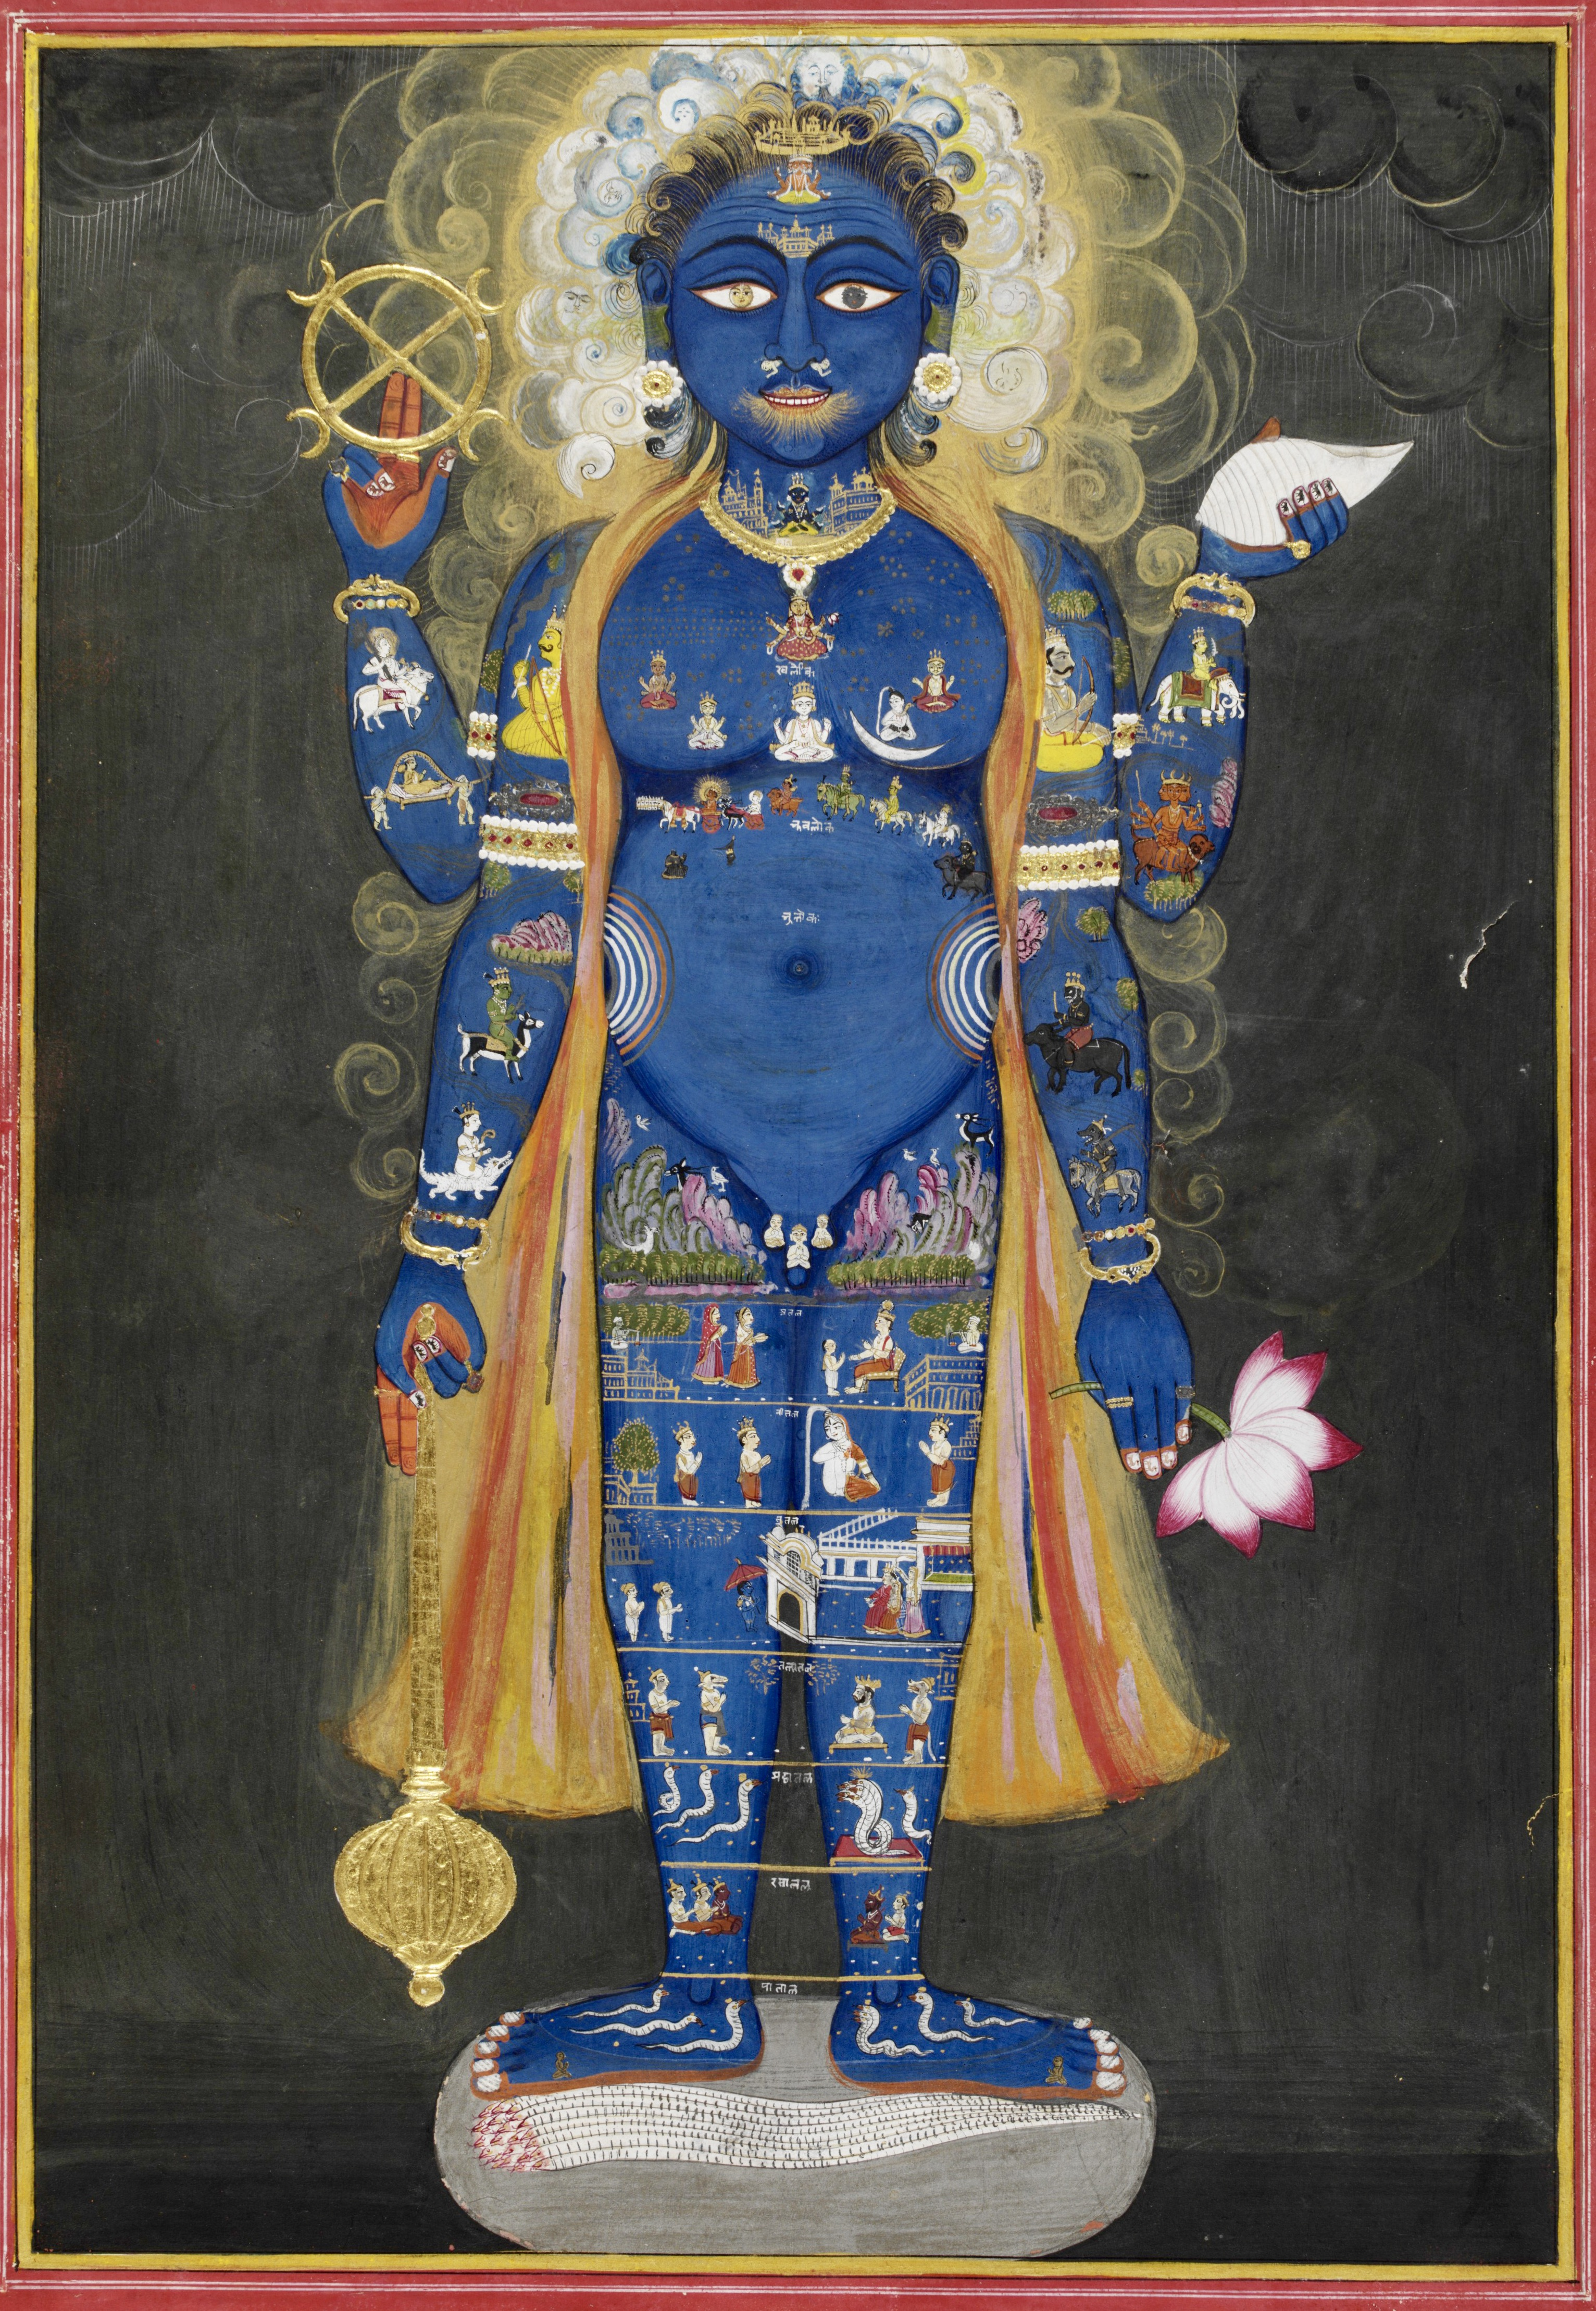
\includegraphics[width=1\textwidth]{pics/Vishnu_Vishvarupa_cropped.jpg}
	\caption{Viṣṇu Viśvarūpa, India, Rajasthan, Jaipur, ca. 1800–1820, Opaque watercolor and gold on paper, 38.5 × 28 cm, Victoria and Albert Museum, London, Given by Mrs. Gerald Clark.}
	\label{fig1}
      \end{figure}
\clearpage
  \begin{figure}[ht]
	\centering
  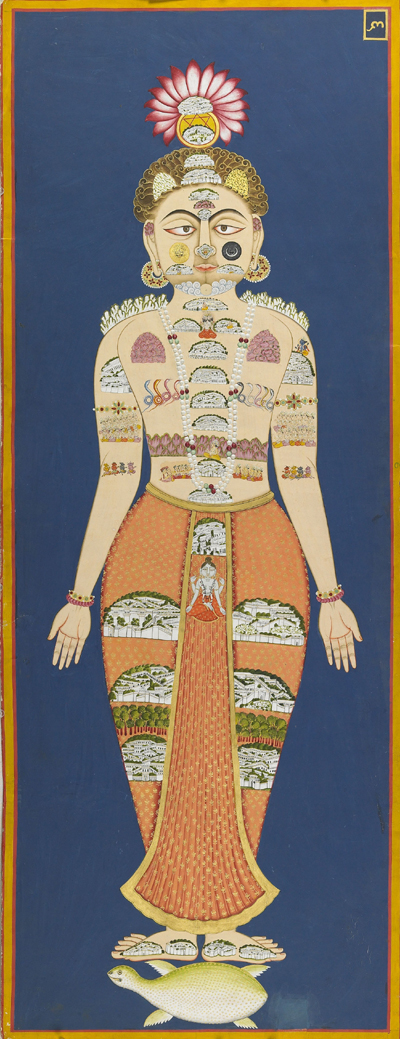
\includegraphics[width=0.5\textwidth]{pics/The_Equivalence_of_Self_and_Universe_(detail),_folio_6_from_the_Siddha_Siddhanta_Paddhati,_(Bulaki),_1824_(Samvat_1881);_122_x_46_cm._Mehrangarh_Museum_Trust..jpg}
	\caption{The Equivalence of Self and Universe (detail), folio 6 from the \textit{Siddhasiddhāntapaddhati} (Bulaki), India, Rajasthan, Jodhpur, 1824 (Samvat 1881), 122 x 46 cm, RJS 2378, Mehragarh Museum Trust.}
	\label{fig2}
      \end{figure}
      % \end{landscape}


\chapter{Bibliography}
 \label{sec:bibli}
   \clearpage
\newpage 
\thispagestyle{empty}
\quad  \addtocounter{page}{-1}

\printbibliography[heading=subbibintoc, title=Consulted Manuscripts, keyword=codex]

\printbibliography[heading=subbibintoc, title=Printed Editions, keyword=printsource]

\printbibliography[heading=subbibintoc, title=Secondary Literature, keyword=seclit]

\printbibliography[heading=subbibintoc, title=Online Sources, keyword=onlinesource]

\end{document}
